% \iffalse meta-comment
%
% Copyright (C) 2005-2021 by Tsinghua University TUNA Association <tuna@tsinghua.edu.cn>
%
% This work may be distributed and/or modified under the
% conditions of the LaTeX Project Public License, either version 1.3c
% of this license or (at your option) any later version.
% The latest version of this license is in
%    https://www.latex-project.org/lppl.txt
% and version 1.3c or later is part of all distributions of LaTeX
% version 2008 or later.
%
% \fi
%
% \iffalse
%<*driver>
\ProvidesFile{bnuthesis.dtx}[2021/05/13 0.0.2 Beijing Normal University Thesis Template]
\documentclass{ltxdoc}
\usepackage{dtx-style}

\EnableCrossrefs
\CodelineIndex

\begin{document}
  \DocInput{\jobname.dtx}
\end{document}
%</driver>
% \fi
%
% \DoNotIndex{\newenvironment,\@bsphack,\@empty,\@esphack,\sfcode}
% \DoNotIndex{\addtocounter,\label,\let,\linewidth,\newcounter}
% \DoNotIndex{\noindent,\normalfont,\par,\parskip,\phantomsection}
% \DoNotIndex{\providecommand,\ProvidesPackage,\refstepcounter}
% \DoNotIndex{\RequirePackage,\setcounter,\setlength,\string,\strut}
% \DoNotIndex{\textbackslash,\texttt,\ttfamily,\usepackage}
% \DoNotIndex{\begin,\end,\begingroup,\endgroup,\par,\\}
% \DoNotIndex{\if,\ifx,\ifdim,\ifnum,\ifcase,\else,\or,\fi}
% \DoNotIndex{\let,\def,\xdef,\edef,\newcommand,\renewcommand}
% \DoNotIndex{\expandafter,\csname,\endcsname,\relax,\protect}
% \DoNotIndex{\Huge,\huge,\LARGE,\Large,\large,\normalsize}
% \DoNotIndex{\small,\footnotesize,\scriptsize,\tiny}
% \DoNotIndex{\normalfont,\bfseries,\slshape,\sffamily,\interlinepenalty}
% \DoNotIndex{\textbf,\textit,\textsf,\textsc}
% \DoNotIndex{\hfil,\par,\hskip,\vskip,\vspace,\quad}
% \DoNotIndex{\centering,\raggedright,\ref}
% \DoNotIndex{\c@secnumdepth,\@startsection,\@setfontsize}
% \DoNotIndex{\ ,\@plus,\@minus,\p@,\z@,\@m,\@M,\@ne,\m@ne}
% \DoNotIndex{\@@par,\DeclareOperation,\RequirePackage,\LoadClass}
% \DoNotIndex{\AtBeginDocument,\AtEndDocument}
%
% \GetFileInfo{\jobname.dtx}
%
% \def\indexname{索引}
% \IndexPrologue{\section{\indexname}}
%
% \title{\bfseries\color{violet}\bnuthesis:北京师范大学学位论文模板}
% \author{{\fangsong 清华大学 TUNA 协会}\\[5pt]\texttt{tuna@tsinghua.edu.cn}}
% \date{v\fileversion\ (\filedate)}
% \maketitle\thispagestyle{empty}
%
%
% \begin{abstract}\noindent
%   此宏包旨在建立一个简单易用的北京师范大学学位论文模板,包括本科综合论文训练、硕士
%   论文、博士论文以及博士后出站报告。
% \end{abstract}
%
% \vskip2cm
% \def\abstractname{免责声明}
% \begin{abstract}
% \noindent
% \begin{enumerate}
% \item 本模板的发布遵守 \href{https://www.latex-project.org/lppl/lppl-1-3c.txt}{\LaTeX{} Project Public License (1.3.c)},使用前请认真阅读协议内
%   容。
% \item 本模板为作者根据
%   清华大学研究生院颁发的《
%    \href{http://yjsy.cic.tsinghua.edu.cn/docinfo/board/boarddetail.jsp?columnId=001050603&parentColumnId=0010506&itemSeq=5365}{%
%   研究生学位论文写作指南}》(限校内网络访问)、
%   英文版《Guide to Thesis Writing for Graduate Students》、
%   清华大学教务处颁发的《
%   \href{https://lib.tsinghua.edu.cn/dra/news/annoucement/7963}{%
%   综合论文训练写作指南}》、
%   外文系的《英语专业本科生综合论文训练》和
%   清华大学《
%   \href{http://postdoctor.tsinghua.edu.cn/info/czxz/1283}{%
%   编写“清华大学博士后研究报告”参考意见}》
%   编写而成,旨在供清华大学毕业生撰写学位论文使用。
% \item 任何个人或组织以本模板为基础进行修改、扩展而生成的新的专用模板,请严格遵
%   守 \LaTeX{} Project Public License 协议。由于违犯协议而引起的任何纠纷争端均与
%   本模板作者无关。
% \end{enumerate}
% \end{abstract}
%
%
% \clearpage
% \pagestyle{fancy}
% \begin{multicols}{2}[
%   \setlength{\columnseprule}{.4pt}
%   \setlength{\columnsep}{18pt}]
%   \tableofcontents
% \end{multicols}
% \clearpage
%
% \section{模板介绍}
% \bnuthesis{}(\textbf{T}sing\textbf{h}ua \textbf{U}niversity \LaTeX{}
% \textbf{Thesis} Template)是为了帮助北京师范大学毕业生撰写毕业论文而编写
% 的 \LaTeX{} 论文模板。
%
% 本文档将尽量完整的介绍模板的使用方法,如有不清楚之处,或者想提出改进建议,
% 可以在 \href{https://github.com/tuna/thuthesis/issues/}{GitHub Issues}
% 参与讨论或提问。
% 有兴趣者都可以参与完善此手册,也非常欢迎对代码的贡献。
%
% \note[注意:]{模板的作用在于减少论文写作过程中格式调整的时间。前提是遵守模板的
% 用法,否则即便用了 \bnuthesis{} 也难以保证输出的论文符合学校规范。}
%
% 用户如果遇到 bug,或者发现与学校《写作指南》 的要求不一致,可以尝试以下办法:
% \begin{enumerate}
%   \item 将模板升级到最新,见第~\ref{sec:upgrade} 节;
%   \item 阅读 \href{https://github.com/tuna/thuthesis/wiki/FAQ}{FAQ};
%   \item 在 GitHub Issues 中按照说明
%     \href{https://github.com/tuna/thuthesis/issues/new?template=bug_report.md}{报告 bug}。
% \end{enumerate}
%
% \section{贡献者}
% \label{sec:contributors}
%
% \bnuthesis{} 的开发过程中,主要的维护者包括:
%
% \begin{itemize}
%  \item 薛瑞尼(\githubuser{xueruini}):最早的开发者,2005 年创建 \bnuthesis{} 并长期进行维护工作。
%  \item 赵涛(\githubuser{alick}):2011-2015 年活跃,较早期阶段的开发者。
%  \item 李泽平(\githubuser{zepinglee}):2016 年至今活跃,为目前主要维护者。
%  \item 陈晟祺(\githubuser{Harry-Chen}):2020 年至今活跃,主要负责非开发性事宜。
% \end{itemize}
%
% 同时,也要感谢所有在 GitHub 上提出问题与贡献代码的同学、老师们。
% \bnuthesis{} 的持续发展,离不开你们的帮助与支持。
%
% \section{安装}
% \label{sec:installation}
%
% \bnuthesis{} 已经包含在主要的 \TeX{} 发行版中,但是通常版本较旧,而且不方便更新。
% 建议从下列途径下载最新版:
% \begin{description}
%  \item[GitHub] \url{https://github.com/tuna/thuthesis},从 Release 中下载 zip 文件。
%  \item[TUNA 镜像站] \url{https://mirrors.tuna.tsinghua.edu.cn/github-release/tuna/thuthesis/},也可在首页选择“获取下载链接——应用软件——\bnuthesis{}论文模板”。
% \end{description}
%
%
% 模板支持在 TeX Live、MacTeX 和 MiKTeX 平台下进行编译,但要求 2017 年或更新的发行版。
% 当然,尽可能使用最新的版本可以避免 bug。
%
% \subsection{模板的组成}
% 下表列出了 \bnuthesis{} 的主要文件及其功能介绍:
%
% \begin{longtable}{l|p{8cm}}
% \toprule
% {\heiti 文件(夹)} & {\heiti 功能描述}\\\midrule
% \endfirsthead
% \midrule
% {\heiti 文件(夹)} & {\heiti 功能描述}\\\midrule
% \endhead
% \endfoot
% \endlastfoot
% bnuthesis.ins & \textsc{DocStrip} 驱动文件(开发用) \\
% bnuthesis.dtx & \textsc{DocStrip} 源文件(开发用)\\\midrule
% bnuthesis.cls & 模板类文件\\
% bnuthesis-*.bst & \hologo{BibTeX} 参考文献表样式文件\\
% bnuthesis-*.bbx & BibLaTeX 参考文献表样式文件\\
% bnuthesis-*.cbx & BibLaTeX 参考文献引用样式文件\\
% bnu-name-bachelor.pdf & 校名 logo,本科生封面使用 \\\midrule
% bnuthesis-example.tex & 示例文档主文件\\
% spine.tex & 书脊示例文档\\
% ref/ & 示例文档参考文献目录\\
% data/ & 示例文档章节具体内容\\
% figures/ & 示例文档图片路径\\
% bnusetup.tex & 示例文档基本配置\\\midrule
% Makefile & Makefile\\
% latexmkrc & latexmk 配置文件 \\
% README.md & Readme\\
% \textbf{bnuthesis.pdf} & 用户手册(本文档)\\\bottomrule
% \end{longtable}
%
% 几点说明:
% \begin{itemize}
% \item \file{bnuthesis.cls} 可由 \file{bnuthesis.ins}
%   和 \file{bnuthesis.dtx} 生成,但为了降低新手用户的使用难度,故
%   将 \file{bnuthesis.cls} 文件一起发布。
% \item 使用前阅读文档:\file{bnuthesis.pdf}。
% \end{itemize}
%
% \subsection{生成模板}
% \label{sec:generate-cls}
% 模板的源文件(\file{bnuthesis.dtx})中包含了大量的注释,需要将注释去掉生成轻量
% 级的 \file{.cls} 文件供 \cs{documentclass} 调用。
%
% \begin{shell}
%   $ xetex bnuthesis.ins
% \end{shell}
%
% \note[注意:]{如果没有生成的模板 \file{bnuthesis.cls} 文件
%   (跟 \file{bnuthesis-example.tex} 同一目录下),
%   \LaTeX{} 在编译时可能找到发行版中较旧版本的 \file{.cls},从而造成冲突。}
%
% \subsection{编译论文}
% \label{sec:generate-thesis}
% 本节介绍几种常见的生成论文的方法。用户可根据自己的情况选择。
%
% 在撰写论文时,我们\textbf{不推荐}使用原有的 \file{bnuthesis-example.tex} 这一名称。
% 建议将其复制一份,改为其他的名字(如 \file{thesis.tex} 或者 \file{main.tex})。
% 需要注意,如果使用了来自 \file{data} 目录中的 \file{tex} 文件,
% 则重命名主文件后,其顶端的 \texttt{!TeX root} 选项也需要相应修改。
%
% \subsubsection{GNU make}
% \label{sec:make}
% 如果用户可以使用 GNU make 工具,这是最方便的办法。
% 所以 \bnuthesis{} 提供了 \file{Makefile}:
% \begin{shell}
%   $ make thesis    # 生成论文示例 bnuthesis-example.pdf
%   $ make spine     # 生成书脊 spine.pdf
%   $ make doc       # 生成说明文档 bnuthesis.pdf
%   $ make clean     # 清理编译生成的辅助文件
% \end{shell}
%
% 需要注意,如果更改了主文件的名称,则需要修改 \file{Makefile} 顶端的 \texttt{THESIS} 变量定义。
%
% \subsubsection{latexmk}
% \label{sec:latexmk}
% \texttt{latexmk} 命令支持全自动生成 \LaTeX{} 编写的文档,并且支持使用不同的工具
% 链来进行生成,它会自动运行多次工具直到交叉引用都被解决。
% \begin{shell}
%   $ latexmk bnuthesis-example.tex  # 生成示例论文 bnuthesis-example.pdf
%   $ latexmk spine.tex              # 生成书脊 spine.pdf
%   $ latexmk bnuthesis.dtx          # 生成说明文档 bnuthesis.pdf
%   $ latexmk -c                     # 清理编译生成的辅助文件
% \end{shell}
% \texttt{latexmk} 的编译过程是通过 \file{latexmkrc} 文件来配置的,如果要进一步了解,
% 可以参考 \pkg{latexmk} 文档。
%
% \subsubsection{\XeLaTeX}
% \label{sec:xelatex}
% 如果用户无法使用以上两种较为方便的编译方法,就只能按照以下复杂的办法手动编译。
%
% 首先,更新模板:
% \begin{shell}
%   $ xetex bnuthesis.ins                       # 生成 bnuthesis.cls
% \end{shell}
%
% 然后,生成论文以及书脊:
% \begin{shell}
%   $ xelatex bnuthesis-example.tex
%   $ bibtex bnuthesis-example.aux              # 生成 bbl 文件
%   $ bibtex bnuthesis-example-survey.aux       # 本科生的调研报告的参考文献
%   $ bibtex bnuthesis-example-translation.aux  # 本科生的外文资料翻译的参考文献
%   $ bibtex bnuthesis-example-index.aux        # 本科生的书面翻译对应的原文索引
%   $ xelatex bnuthesis-example.tex             # 解决引用
%   $ xelatex bnuthesis-example.tex             # 生成论文 PDF
%
%   $ xelatex spine.tex                         # 生成书脊 PDF
% \end{shell}
%
% 在调用 \XeLaTeX 时,如果设置了 \option{include-spine} 选项,
% 则需要在文件名前加上 \texttt{-shell-scape} 的命令行选项。
%
% 下面的命令用来生成用户手册:
% \begin{shell}
%   $ xelatex -shell-escape bnuthesis.dtx
%   $ makeindex -s gind.ist -o bnuthesis.ind bnuthesis.idx
%   $ xelatex -shell-escape bnuthesis.dtx
%   $ xelatex -shell-escape bnuthesis.dtx  # 生成说明文档 bnuthesis.pdf
% \end{shell}
%
% \subsection{升级}
% \label{sec:upgrade}
% 如果需要升级 \bnuthesis{},应当从 GitHub 下载最新的版本,
% 将 \file{bnuthesis.dtx},\file{bnuthesis.ins},\file{bnu-name-bachelor.pdf} 和
% \file{bnuthesis-*.bst} 拷贝至工作目录覆盖相应的文件,然后按照
% 第~\ref{sec:generate-cls} 节的内容生成新的模板和使用说明。
%
% 有时模板可能进行了重要的修改,不兼容已写好的正文内容,用户应按照示例
% 文档重新调整。
%
% \section{使用说明}
% \label{sec:usage}
% 本手册假定用户已经能处理一般的 \LaTeX{} 文档,并对 \hologo{BibTeX} 有一定了解。如果
% 从未接触过 \TeX{} 和 \LaTeX,建议先学习相关的基础知识。
%
% \subsection{示例文件}
% \label{sec:userguide}
%
% 模板核心文件有:\file{bnuthesis.cls},\file{bnu-name-bachelor.pdf},
% \file{bnuthesis-*.bst}(\hologo{BibTeX}),
% \file{bnuthesis-*.bbx} 和 \file{bnuthesis-*.cbx}(BibLaTeX),
% 但如果没有示例文档会较难下手,所以推荐从模板自带的示例文档入手。其中包括了论文
% 写作用到的所有命令及其使用方法,只需用自己的内容进行相应替换就可以。对于不清
% 楚的命令可以查阅本手册。下面的例子描述了模板中章节的组织形式,来自于示例文档,
% 具体内容可以参考模板附带的 \file{bnuthesis-example.tex} 和 \file{data/}。
%
% \subsection{论文选项}
% \label{sec:option}
%
% \subsubsection{学位}
% \DescribeOption{degree}
% 选择学位,可选:
% \option{bachelor},\option{master},\option{doctor}(默认),\option{postdoc}。
% 本节中的 \emph{key-value} 选项只能在文档类的选项中进行设置,
% 不能用于 \cs{bnusetup} 命令。
% \begin{latex}
%   % 博士论文
%   \documentclass[degree=doctor]{bnuthesis}
% \end{latex}
%
% \subsubsection{学位类型}
% \label{sec:degree-type}
% \DescribeOption{degree-type}
% 定义研究生学位的类型,可选:\option{academic}(默认)、\option{professional},
% 本科生不受影响。
% \begin{latex}
%   \documentclass[degree=master, degree-type=professional]{bnuthesis}
% \end{latex}
%
% \subsubsection{字体配置}
% \label{sec:font-config}
% \DescribeOption{fontset}
% 模板默认会自动根据操作系统配置合适的字体,
% 用户也可以通过 \option{fontset} 时指定使用预设的字库,如:
% \begin{latex}
%   \documentclass[fontset=windows]{bnuthesis}
% \end{latex}
% 允许的选项有 \option{windows}、\option{mac}、\option{ubuntu} 和 \option{fandol},
% 具体使用的字体见表~\ref{tab:fontset}。
% 用户也可以设置为 \option{none} 并自行配置字体。
%
% \begin{table}[htb]
%   \centering
%   \caption{\bnuthesis{} 预设的字体}
%   \label{tab:fontset}
%   \begin{tabular}{cccc}
%     \toprule
%     \option{windows} & \option{mac}    & \option{ubuntu} & \option{fandol} \\
%     \midrule
%     Times New Roman  & Times New Roman & TeX Gyre Termes & TeX Gyre Termes \\
%     Arial            & Arial           & TeX Gyre Heros  & TeX Gyre Heros  \\
%     Courier          & Menlo           & TeX Gyre Cursor & TeX Gyre Cursor \\
%     中易宋体         & 华文宋体        & 思源宋体        & Fandol 宋体     \\
%     中易黑体         & 华文黑体        & 思源黑体        & Fandol 黑体     \\
%     \bottomrule
%   \end{tabular}
% \end{table}
%
% 需要注意,研究生院建议中文字体同 Word 模板一致。
% 也就是说,用户在提交终版前应使用 Windows 平台的字体进行编译。
%
% 关于字体的配置,
% 详见 \pkg{fontspec}、\pkg{xeCJK}、\pkg{ctex} 等宏包的使用说明和代码。
%
%
% \subsection{论文设置}
% 论文的设置可以通过统一命令 \cs{bnusetup} 设置 \emph{key=value} 形式完成。
%
% \DescribeMacro{\bnusetup}
% \cs{bnusetup} 用法与常见 \emph{key=value} 命令相同,如下:
% \begin{latex}
%   \bnusetup{
%     key1 = value1,
%     key2 = {a value, with comma},
%   }
%   % 可以多次调用
%   \bnusetup{
%     key3 = value3,
%     key1 = value11,  % 覆盖 value1
%   }
% \end{latex}
%
% \note[注意:]{\cs{bnusetup} 使用 \pkg{kvsetkeys} 机制,所以配置项之间不能有空行,否则
% 会报错。}
%
% \subsubsection{输出格式}
% \DescribeOption{output}
% 选择输出的格式是打印版还是电子版(用于提交),可选:\option{print}(默认)、\option{electronic}。
% 一些院系要求提交的电子版不含空白页,但是这对打印并不友好,
% 比如正文第一页可能会在左侧;以及一些部分需要单面打印,需要插入空白页。
% 注意在不同选项下,生成的声明页码很可能不同。为了避免页码错误,
% \bnuthesis{}将会在插入扫描的 PDF 文件时自动生成页码,因此\textbf{扫描声明页时请移除底部的页码},以防重叠。
%
% \begin{latex}
%   \bnusetup{
%     output = electronic,
%   }
% \end{latex}
%
% 另外本科生要求有 0.2cm 留给装订线的宽度,这只有在打印版中才会生效。
%
%
% \subsubsection{书写语言}
% \DescribeOption{language}
% 在导言区设置 \option{language} 会修改论文的主要语言,如章节标题等。
% 在正文中设置 \option{language} 只修改接下来部分的书写语言,
% 如标点格式、图表名称,但不影响章节标题等。
%
% \begin{latex}
%   \bnusetup{
%     language = english,
%   }
% \end{latex}
%
% 论文的一些部分(如英文摘要、本科生的外文调研报告)要求使用特定的语言,
% 模板已经进行配置,并在这些部分结束后自动恢复为主要语言。
%
% 注意,本科生《写作指南》要求“本科生(含国外来华留学本科生)非外语专业论文统一要求
% 用中文书写。”研究生《写作指南》要求“外国人来华留学生可以用英文撰写学位论文,但
% 须采用中文封面”,“除留学生外,学位论文一律须用汉语书写”,用户须提前与导师和院系
% 的审查教师协商使用何种语言书写论文。
%
% \subsubsection{开题报告}
% \DescribeOption{thesis-type}
% 模板还支持博士生论文开题报告的格式,可以通过设置 \option{thesis-type=proposal} 得到。
%
% 开题报告与学位论文有两点不同:
% \begin{enumerate}
%   \item 封面的信息和格式有区别,尤其是增加了一行“学号”信息,需要通过 \option{student-id} 填写;
%   \item 开题报告不含英文标题页。
% \end{enumerate}
% \begin{latex}
%   \bnusetup{
%     thesis-type = proposal,
%     student-id  = {2000310000},
%   }
% \end{latex}
%
% \subsection{封面信息}
% \label{sec:titlepage}
% 封面信息可以通过统一设置命令 \cs{bnusetup} 设置 \emph{key=value} 形式完成;
% 带 * 号的键通常是对应的英文。
%
% \subsubsection{论文标题}
% 中英文标题。可以在标题内部使用换行|\\|。
% \begin{latex}
%   \bnusetup{
%     title  = {论文中文题目},
%     title* = {Thesis English Title},
%   }
% \end{latex}
%
% \subsubsection{申请学位名称}
% \label{sec:degree-name}
% 学位名称的设置比较复杂,见表~\ref{tab:degree-name}。
%
% \begin{table}[h]
%   \caption{学位名称的要求}
%   \label{tab:degree-name}
%   \begin{tabular}{p{2cm}p{6cm}p{6cm}}
%     \toprule
%     学位类型 & degree-name & degree-name* \\
%     \midrule
%     学术型博士 & 需注明所属的学科门类,例如:
%         哲学、经济学、法学、教育学、文学、历史学、理学、工学、农学、医学、
%         军事学、管理学、艺术学
%       & Doctor of Philosophy \\
%     \midrule
%     学术型硕士 & 同上
%       & 哲学、文学、历史学、法学、教育学、艺术学门类,公共管理学科
%         填写“Master of Arts“,其它填写“Master of Science” \\
%     \midrule
%     专业型研究生学位 & 专业学位的名称,例如:教育博士、工程硕士
%       & 专业学位的名称,例如:Doctor of Education, Master of Engineering \\
%     \midrule
%     本科生 & - & - \\
%     \bottomrule
%   \end{tabular}
% \end{table}
%
% \begin{latex}
%   \bnusetup{
%     degree-name  = {您要申请什么学位},
%     degree-name* = {Degree in English},
%   }
% \end{latex}
%
% \subsubsection{院系名称}
% 院系名称。
% \begin{latex}
%   \bnusetup{
%     department = {系名全称},
%   }
% \end{latex}
%
% \subsubsection{学科名称}
%
% \begin{itemize}
%   \item 学术型学位:获得一级学科授权的学科填写一级学科名称,其他填写二级学科名称;
%   \item 工程硕士:工程领域名称;
%   \item 其他专业型学位:-
%   \item 本科生:专业名称,第二学位论文需标注“(第二学位)”
% \end{itemize}
%
% \begin{latex}
%   \bnusetup{
%     discipline  = {学科名称},
%     discipline* = {Discipline in English},
%   }
% \end{latex}
%
% \subsubsection{作者姓名}
% 作者姓名。
% \begin{latex}
%   \bnusetup{
%     author  = {中文姓名},
%     author* = {Name in Pinyin},
%   }
% \end{latex}
%
% \subsubsection{学号}
% 学号,仅用于博士生论文开题报告。
% \begin{latex}
%   \bnusetup{
%     student-id  = {20000310000},
%   }
% \end{latex}
%
% \subsubsection{导师}
% \myentry{导师}
% 导师的姓名与super之间以“,”(西文逗号,U+002C)隔开,下同。
% \begin{latex}
%   \bnusetup{
%     supervisor  = {导师姓名, 教授},
%     supervisor* = {Professor Supervisor Name},
%     supervisor-department = {导师单位},
%   }
% \end{latex}
%
% \myentry{副导师}
% 本科生的辅导教师,硕士的副指导教师。
% \begin{latex}
%   \bnusetup{
%     associate-supervisor  = {副导师姓名, 副教授},
%     associate-supervisor* = {Professor Assoc-Supervisor Name},
%   }
% \end{latex}
%
% \myentry{联合导师}
% 硕士生、本科生联合指导教师,博士生联合导师。
% \begin{latex}
%   \bnusetup{
%     co-supervisor  = {联合导师姓名, 教授},
%     co-supervisor* = {Professor Join-Supervisor Name},
%   }
% \end{latex}
%
% \subsubsection{成文日期}
% 默认为当前日期,也可以自己指定,要求使用 ISO 格式。
% \begin{latex}
%   \bnusetup{
%     date = {2011-07-01},
%   }
% \end{latex}
%
% \subsubsection{密级}
% \label{sec:setup-secret}
% 定义秘密级别和年限。
% \begin{latex}
%   \bnusetup{
%     secret-year  = 10,
%     secret-level = {秘密},
%   }
% \end{latex}
%
% \subsubsection{博士后专用参数}
% \begin{latex}
%   \bnusetup{
%     clc                = {分类号},
%     udc                = {udc},
%     id                 = {id},
%     discipline-level-1 = {流动站(一级学科)名称},
%     discipline-level-2 = {专业(二级学科)名称},
%     start-date         = {2011-07-01}, % 研究工作起始时间
%   }
% \end{latex}
%
% \myentry{生成封面}
% \DescribeMacro{\maketitle}
% 生成封面,不含授权说明,摘要等。
% \begin{latex}
%   % 直接生成封面
%   \maketitle
% \end{latex}
%
% \subsection{前言部分}
%
% \subsubsection{指导小组、公开评阅人和答辩委员会名单}
% \myentry{答辩委员会名单}
% \DescribeEnv{committee}
% 学位论文指导小组、公开评阅人和答辩委员会名单可以由 \env{committee} 环境生成,
% 其中的可选参数可以使用 \option{name} 根据是有无指导小组设置合适的标题,比如
% \begin{latex}
%   \begin{committee}[name={学位论文公开评阅人和答辩委员会名单}]
%     ...
%   \end{committee}
% \end{latex}
%
% 答辩委员会名单中的表格使用 LaTeX 生成可能略麻烦,也可以导入 Word 版转成的 PDF 文件,
% \begin{latex}
%   \begin{committee}[file=figures/committee.pdf]
%   \end{committee}
% \end{latex}
%
% \subsubsection{授权说明}
% \myentry{授权说明}
% \DescribeMacro{\copyrightpage}
% 可选参数为扫描得到的 PDF 文件名,例如:
% \begin{latex}
%   % 将签字扫描后授权文件 scan-copyright.pdf 替换原始页面
%   \copyrightpage[file=scan-copyright.pdf]
% \end{latex}
%
% \subsubsection{摘要}
% \myentry{摘要正文}
% \DescribeEnv{abstract}
% \DescribeEnv{abstract*}
%
% 摘要直接在正文中使用 \env{abstract}、\env{abstract*} 环境生成。
%
% \begin{latex}
%   \begin{abstract}
%     摘要请写在这里...
%   \end{abstract}
%
%   \begin{abstract*}
%     Here comes the abstract in English...
%   \end{abstract*}
% \end{latex}
%
% \myentry{关键词}
% 关键词需要使用 \cs{bnusetup} 进行设置。关键词之间以\emph{西文逗号}隔开,模板会
% 自动调整为要求的格式。关键词的设置只要在摘要环境结束前即可。
% \begin{latex}
%   \bnusetup{
%     keywords  = {关键词 1, 关键词 2},
%     keywords* = {keyword 1, keyword 2},
%   }
% \end{latex}
%
% \subsubsection{目录和索引表}
% 目录、插图、表格、公式和算法等索引命令分别如下,将其插入到期望的位置即可(带*的命令表
% 示对应的索引表不会出现在目录中):
%
% \DescribeMacro{\tableofcontents}
% \DescribeMacro{\listoffigures}
% \DescribeMacro{\listoffigures*}
% \DescribeMacro{\listoftables}
% \DescribeMacro{\listoftables*}
% \DescribeMacro{\listofequations}
% \DescribeMacro{\listofequations*}
% \DescribeMacro{\listofalgorithms}
% \DescribeMacro{\listofalgorithms*}
% \begin{longtable}{ll}
% \toprule
%   {\heiti 用途} & {\heiti 命令} \\\midrule
% 目录     & \cs{tableofcontents} \\\midrule
% 插图索引 & \cs{listoffigures}   \\
%          & \cs{listoffigures*}  \\\midrule
% 表格索引 & \cs{listoftables}    \\
%          & \cs{listoftables*}   \\\midrule
% 公式索引 & \cs{listofequations} \\
%          & \cs{listofequations*}\\\midrule
% 算法索引 & \cs{listofalgorithms} \\
%          & \cs{listofalgorithms*}\\\bottomrule
% \end{longtable}
%
% \DescribeOption{toc-chapter-style}
% 本科生《写作指南》关于目录章标题要求“目录从第 1 章开始,每章标题用黑体小四号字”,
% 所以其中的西文和数字默认使用 Arial 字体,跟正文的章标题一致。
% 但是论文样例\footnote{
%   \url{http://www.law.tsinghua.edu.cn/publish/law/7024/2012/20120216153516317135347/20120216153516317135347_.html}
% }的目录章标题的西文和数字却使用了 Times。
% 如果审查老师这样要求,需要在生成目录前设置
% \begin{latex}
%   \bnusetup{
%     toc-chapter-style = times,
%   }
% \end{latex}
% 该选项只对本科生有效。
%
% \LaTeX{} 默认支持插图和表格索引,是通过 \cs{caption} 命令完成的,因此它们必须出
% 现在浮动环境中,否则不被计数。
%
% 如果不想让某个表格或者图片出现在索引里面,那么请使用命令 \cs{caption*},这
% 个命令不会给表格编号,也就是出来的只有标题文字而没有“表~xx”,“图~xx”,否则
% 索引里面序号不连续就显得不伦不类,这也是 \LaTeX{} 里星号命令默认的规则。
%
% 如果的确想让其编号,但又不想出现在索引中的话,目前模板暂不支持。
%
% 公式索引为本模板扩展,模板扩展了 \pkg{amsmath} 几个内部命令,使得公式编号样式和
% 自动索引功能非常方便。一般来说,你用到的所有数学环境编号都没问题了,这个可以参
% 看示例文档。如果你有个非常特殊的数学环境需要加入公式索引,那么请使
% 用 \cs{equcaption}\marg{编号}。此命令表示 equation caption,带一个参数,即显示
% 在索引中的编号。因为公式与图表不同,我们很少给一个公式附加一个标题,之所以起这
% 么个名字是因为图表就是通过 \cs{caption} 加入索引的,\cs{equcaption} 完全就是为
% 了生成公式列表,不产生什么标题。
%
% 使用方法如下。假如有一个非 equation 数学环境 \texttt{mymath},只要在其中写一
% 句 \cs{equcaption} 就可以将它加入公式列表。
% \begin{latex}
%   \begin{mymath}
%     \label{eq:emc2}\equcaption{\ref{eq:emc2}}
%     E=mc^2
%   \end{mymath}
% \end{latex}
%
% \texttt{mymath} 中公式的编号需要自己来做。
%
% 同图表一样,附录中的公式有时也不希望它跟全文统一编号,而且不希望它出现在公式
% 索引中。目前的办法是利用 \cs{tag*}\marg{公式编号} 来解决。用法比较简单,此
% 处不再罗嗦,实例请参看示例文档附录 A 的前两个公式。
%
% \subsubsection{符号对照表}
% \DescribeEnv{denotation}
% 主要符号表环境,跟 \env{description} 类似,使用方法参见示例文件。带一个可选参数,
% 用来指定符号列的宽度(默认为 2.5cm)。
% \begin{latex}
%   \begin{denotation}
%     \item[E] 能量
%     \item[m] 质量
%     \item[c] 光速
%   \end{denotation}
% \end{latex}
%
% 如果默认符号列的宽度不满意,可以通过参数来调整:
% \begin{latex}
%   \begin{denotation}[1.5cm] % 设置为 1.5cm
%     \item[E] 能量
%     \item[m] 质量
%     \item[c] 光速
%   \end{denotation}
% \end{latex}
%
% 符号对照表的另外一种方法是调用 \pkg{nomencl} 宏包,需要在导言区设置:
%
% \begin{latex}
%   \usepackage{nomencl}
%   \makenomenclature
% \end{latex}
%
% 然后在正文中任意位置使用 \cs{nomenclature} 声明需要添加到主要符号表的符号:
%
% \begin{latex}
%   \nomenclature{$m$}{The mass of one angel}
% \end{latex}
%
% 最后使用 \cs{printnomenclature} 命令生成符号表。更详细的使用方法参
% 见 \pkg{nomencl} 宏包的文档。
%
% \subsection{正文部分}
% \subsubsection{图表编号}
% \DescribeOption{figure-number-separator}
% \DescribeOption{table-number-separator}
% \DescribeOption{equation-number-separator}
% 本科生要求公式的编号使用“-”连接。
% 
% 研究生要求图表和公式的编号使用“.”或“-”连接,模板默认使用句点“.”。
% 用户也可以通过 \option{figure-number-separator}、\option{table-number-separator}
% 等选项分别设置:
% \begin{latex}
%   \bnusetup{
%     figure-number-separator = {-},
%     table-number-separator = {-},
%     equation-number-separator = {-},
%   }
% \end{latex}
% \DescribeOption{number-separator}
% 也可以使用 \option{number-separator} 同时设置图、表、公式三项的编号连接符,
% 比如 |\bnusetup{number-separator = -}|。
%
% 本科生要求“附录中图、表、公式的编号,应与正文中的编号区分开”,
% 应理解为将章号改变为附录对应的大写字母编号,连接符不宜改变。
%
% \subsubsection{数学符号}
% \label{sec:math}
% 中文论文的数学符号默认遵循 GB/T 3102.11—1993《物理科学和技术中使用的数学符号》
% \footnote{原 GB 3102.11—1993,自 2017 年 3 月 23 日起,该标准转为推荐性标准。}。
% 该标准参照采纳 ISO 31-11:1992 \footnote{目前已更新为 ISO 80000-2:2019。},
% 但是与 \TeX{} 默认的美国数学学会(AMS)的习惯有许多差异。
% 这将在下文详细论述。
%
% \DescribeOption{math-style}
% 用户可以通过设置 \option{math-style} 选择数学符号样式(可选:
% \option{GB}(中文默认),\option{TeX}(英文默认)和 \option{ISO}),比如:
% \begin{latex}
%   \bnusetup{
%     math-style = ISO,
%   }
% \end{latex}
%
% 用户也可以逐项修改数学样式。
% \newcommand\dif{\mathop{}\!\mathrm{d}}
% \begin{enumerate}
%   \item \DescribeOption{uppercase-greek}
%     大写希腊字母的正/斜体,可选:\option{italic}、\option{upright}。
%     有限增量符号 $\increment x$ 固定使用正体,推荐使用 \cs{increment} 表示。
%   \item \DescribeOption{less-than-or-equal}
%     小于等于号和大于等于号的字形,可选:\option{slanted}、\option{horizontal}。
%     这将控制 \cs{le}、\cs{ge}、\cs{leq} 和 \cs{geq} 的符号
%     是“$\leqslant$、$\geqslant$”还是“$\leq$、$\geq$”。
%   \item \DescribeOption{integral}
%     积分号的正/斜体,可选:\option{upright}、\option{slanted}。
%     该选项需要字体的支持,目前仅限 \option{xits}、\option{stix}、
%     \option{libertinus} 和 \option{newcm}。参考下文关于数学字体的选择。
%   \item \DescribeOption{integral-limits}
%     积分号上下限的位置,可选:\option{true}(在上下)、\option{false}(在右侧)。
%     这个设置只影响行间公式,行内公式统一居右侧,不受影响。
%   \item \DescribeOption{partial}
%     偏微分符号的正/斜体,可选:\option{upright}、\option{slanted}。
%   \item \DescribeOption{math-ellipsis}
%     省略号 \cs{dots} 的样式,可选:\option{centered}(按照中文的习惯固定居中)、
%     \option{lower} 和 \option{AMS}(取决于前后符号的位置)。
%     其他的省略号命令如 \cs{lots}、\cs{cdots} 则不受影响。
%   \item \DescribeOption{real-part}
%     实部 \cs{Re} 和虚部 \cs{Im} 的字体,可选:\option{roman} 和 \option{fraktur}。
% \end{enumerate}
%
% 如果数学符号选择国标样式 |math-style = GB|,相当于设置了
% \begin{latex}
%   \bnusetup{
%     uppercase-greek    = italic,
%     less-than-or-equal = slanted,
%     integral           = upright,
%     integral-limits    = true,
%     partial            = upright,
%     math-ellipsis      = centered,
%     real-part          = roman,
%   }
% \end{latex}
%
% 另外,国标的数学样式与 AMS 还有一些差异无法统一设置,需要用户在写作时进行处理。
% \begin{enumerate}
%   \item 数学常数和特殊函数名用正体,如 $\uppi = 3.14\dots$;$\symup{i}^2 = -1$;
%     $\symup{e} = \lim_{n \to \infty} \left( 1 + \frac{1}{n} \right)^n$。
%   \item 微分号使用正体,比如 $\dif y / \dif x$。
%   \item 向量、矩阵和张量用粗斜体(\cs{symbf}),如 $\symbf{x}$、$\symbf{\Sigma}$、$\symbfsf{T}$。
% \end{enumerate}
%
% 需要注意,上述关于数学符号风格的设置在设置数学字体(\option{math-font})时才会生效。
%
% \DescribeOption{math-font}
% 模板使用默认使用 XITS Math 作为数学字体。
% 用户也可以使用 \option{math-font} 选项切换其他数学字体,可选:
% \option{stix}(STIX Two Math)、
% \option{libertinus}(Libertinus Math)、
% \option{newcm}(New Computer Modern Math)、
% \option{lm}(Latin Modern Math)。
%
% 其中 \option{lm} 和 \option{newcm} 的字形比较搭配 TeX 原生的 Computer Modern 字体,
% 但与《指南》要求的西文字体 Times New Roman 并不搭配。
% 可能会造成正文和公式中的数字字体不一致,需要谨慎使用。
%
% 以上字体都是 OpenType 格式的字体,需要配合
% \href{http://mirrors.ctan.org/macros/latex/contrib/unicode-math/unicode-math.pdf}{\pkg{unicode-math}}
% 宏包使用。
% 全部数学符号的命令参考
% \href{http://mirrors.ctan.org/macros/latex/contrib/unicode-math/unimath-symbols.pdf}{\pkg{unimath-symbols}}。
% 注意,\pkg{unicode-math} 宏包与 \pkg{amsfonts}、\pkg{amssymb}、\pkg{bm}、
% \pkg{mathrsfs}、\pkg{upgreek} 等宏包\emph{不}兼容。
% 模板作了处理,用户可以直接使用这些宏包的命令,如 \cs{bm}、\cs{mathscr}、
% \cs{uppi}。
%
% 另外,模板还为 `math-font` 提供了传统的 Type 1 字体 \option{newtx}。
% 该选项会调用 \pkg{newtxmath} 宏包。
% 但是,如果西文字体已经使用了 OpenType 的 Times New Roman,
% 混用 Type 1 字体可能会导致问题,尤其是使用 \pkg{siunitx} 宏包时。
% 该选项还处于测试阶段,需要谨慎使用。
%
% \subsubsection{定理环境}
% \label{sec:theorem}
% \bnuthesis{} 定义了常用的数学环境:
%
% \begin{center}
% \begin{tabular}{*{7}{l}}\toprule
%   axiom & theorem & definition & proposition & lemma & conjecture &\\
%   公理 & 定理 & 定义 & 命题 & 引理 & 猜想 &\\\midrule
%   proof & corollary & example & exercise & assumption & remark & problem \\
%   证明 & 推论 & 例子& 练习 & 假设 & 注释 & 问题\\\bottomrule
% \end{tabular}
% \end{center}
%
% 比如:
% \begin{latex}
%   \begin{definition}
%     道千乘之国,敬事而信,节用而爱人,使民以时。
%   \end{definition}
% \end{latex}
% 产生(自动编号):
% \medskip
%
% \noindent\framebox[\linewidth][l]{{\heiti 定义~1.1~~~} % {道千乘之国,敬事而信,节用而爱人,使民以时。}}
%
% \smallskip
% 列举出来的数学环境毕竟是有限的,如果想用\emph{胡说}这样的数学环境,那么可以定义:
% \begin{latex}
%   \newtheorem{nonsense}{胡说}[chapter]
% \end{latex}
%
% 然后这样使用:
% \begin{latex}
%   \begin{nonsense}
%     契丹武士要来中原夺武林秘笈。—— 慕容博
%   \end{nonsense}
% \end{latex}
%
% 产生(自动编号):
%
% \medskip
% \noindent\framebox[\linewidth][l]{{\heiti 胡说~1.1~~~} % {契丹武士要来中原夺武林秘笈。—— 慕容博}}
%
% \subsubsection{列表环境}
% \DescribeEnv{itemize}
% \DescribeEnv{enumerate}
% \DescribeEnv{description}
% 为了适合中文习惯,模板将这三个常用的列表环境用 \pkg{enumitem} 进行了纵向间距压
% 缩。一方面清除了多余空间,另一方面用户可以自己指定列表环境的样式(如标签符号,
% 缩进等)。细节请参看 \pkg{enumitem} 文档,此处不再赘述。
%
% \subsubsection{引用方式}
% \label{sec:citestyle}
% 模板支持两种引用方式,分别为理工科常用的“顺序编码制”和文科常用
% 的“著者-出版年制”。
% 使用者在设置参考文献表的格式
% (\cs{bibliographystyle},见第~\ref{sec:bibliography} 节)时,
% 正文中引用文献的标注会自动调整为对应的格式。
%
% 如果需要标出引文的页码,可以写在 \cs{cite} 的可选参数中,如
% |\cite[42]{knuth84}|。
%
% \paragraph{顺序编码制}
% \DescribeMacro{\inlinecite}
% 顺序编码制的参考文献引用分为两种模式:
% \begin{enumerate}
%   \item 上标模式,比如“同样的工作有很多\textsuperscript{[1-2]}……”;
%   \item 正文模式,比如“文 [3] 中详细说明了……”。
% \end{enumerate}
%
% \DescribeOption{cite-style}
% 用户可以将引用标注的格式设为正文模式:
% \begin{latex}
%   \bnusetup{
%     cite-style = inline,
%   }
% \end{latex}
% 也可以使用 \cs{inlinecite}\marg{key} 临时使用正文模式的引用标注。
%
% \paragraph{著者-出版年制}
% 著者-出版年制的参考文献引用有两种模式:
% \begin{enumerate}
%   \item \cs{citep}:著者与年份均在括号中,比如“(Zhang, 2008)”,
%     同默认的 \cs{cite} 命令;
%   \item \cs{citet}:著者姓名作为正文的一部分,比如“Zhang (2008)”;
% \end{enumerate}
%
% 另外,\pkg{natbib} 还提供了其他方便引用的命令,
% 比如 \cs{citeauthor}、\cs{citeyear} 等,
% 更多细节参考 \pkg{natbib} 的文档。
%
% \subsection{其他部分}
%
% \subsubsection{参考文献}
% \label{sec:bibliography}
%
% 参考文献通常可以使用 \hologo{BibTeX} 或 biblatex 生成。
% \hologo{BibTeX} 是 LaTeX 处理参考文献的传统的方式,
% 需要在使用 \cs{bibliographystyle}\marg{style} 选择样式
% 并用 \cs{bibliography} 设置 \file{.bib} 的路径。
% 然后使用 \texttt{bibtex} 对 \file{.aux} 文件进行编译得到 \file{.bbl} 文件。
% 其中的参考文献表内容会在后续编译时替换到 \cs{bibliography} 的位置。
% Biblatex 是较新的方式,需要在载入宏包时通过 \option{style} 选择样式,
% 在导言区使用 \cs{addbibresource} 声明数据库的路径,
% 并在输出参考文献表的位置使用 \cs{printbibliography} 命令,
% 而且编译参考文献的命令需要换为 biber。
% 这两种方式各有优缺点,比如 BibTeX 无法对中文按照拼音排序,一些样式更新不够及时;
% Biblatex 运行较缓慢,无法对多个参考文献表使用不同样式。
% 用户需要根据实际选择合适的方式。
%
% 研究生要求的参考文献格式基于《信息与文献 参考文献著录规则》(GB/T 7714—2015)
% 进行了少量改编(如英文姓名不使用全大写),
% 可以选择“顺序编码制”和“著者-出版年制”。
% 如果使用 BibTeX 的方式,需要在导言区载入 \pkg{natbib} 宏包并选择样式,如:
% \begin{latex}
%   % 顺序编码制
%   \usepackage[sort]{natbib}
%   \bibliographystyle{bnuthesis-numeric}
% \end{latex}
% 或
% \begin{latex}
%   % 著者-出版年制
%   \usepackage{natbib}
%   \bibliographystyle{bnuthesis-author-year}
% \end{latex}
% 其中的 \option{sort} 选项会将同一处引用的多个文献编号严格按照顺序排序,
% 这并非《写作指南》要求,但是推荐使用。
% 这里调用的样式由 \href{http://ctan.org/pkg/gbt7714}{\pkg{gbt7714}} 的 \file{.bst} 进行了少量修改。
%
% 参考文献表采用“著者-出版年”制组织时,各篇文献首先按文种集中,然后按著者字
% 顺和出版年排列;中文文献可以按著者汉语拼音字顺排列,也可以按著者的笔画笔顺排列。
% 但由于 \hologo{BibTeX} 功能的局限性,无法自动获取著者姓名的拼音或笔画笔顺进行正确排序。
% 一种解放方法是在 \file{.bib} 数据库的中文文献的 |key| 域手动录入著者姓名的拼音,
% 这比较适合中文文献数量较少的情况,如:
% \begin{latex}
%   @book{capital,
%     author = {马克思 and 恩格斯},
%     key    = {ma3 ke4 si1 & en1 ge2 si1},
%     ...
%   }
% \end{latex}
% 另一种方式是使用 biblatex,应在在导言区设置
% \begin{latex}
%   \usepackage[backend=biber,style=bnuthesis-author-year]{biblatex}
%   \addbibresource{ref/refs.bib}
% \end{latex}
% 这里的样式由 \href{https://ctan.org/pkg/biblatex-gb7714-2015}{biblatex-gb7714-2015} 进行了少量改编,
% 一些额外用法可以参考该宏包的文档。
% 注意 \pkg{biblatex} 跟 \pkg{natbib} 不兼容,
% 而且 \cs{addbibresource} 必须在导言区设置。
% 输出参考文献表应使用 \cs{printbibliography} 命令。
%
% 本科生要求的中文参考文献格式严格遵从 GB/T 7714—2015,
% 附录中调研报告的英文参考文献可以自行选择合适的风格。
% 但是 biblatex 不支持同一文档中使用不同的格式,
% 所以只能使用 \hologo{BibTeX}:
% \begin{latex}
%   % 本科生参考文献的著录格式
%   \usepackage[sort]{natbib}
%   \bibliographystyle{bnuthesis-bachelor}
% \end{latex}
% 调研报告的参考文献需要选择与 \pkg{natbib} 兼容的样式。
%
% 本科生外文系要求使用 APA 或 MLA。
% APA 的 BibTeX 样式由 \pkg{apacite} 宏包提供,需要在导言区调用:
% \begin{latex}
%   \usepackage[natbibapa]{apacite}
%   \bibliographystyle{apacite}
% \end{latex}
% 其中 \option{natbibapa} 会调用 \pkg{natbib} 来处理引用,
% 这也是宏包推荐的用法。
% 注意目前的 \pkg{apacite} 只支持到 APA 第 6 版。
% 更推荐使用已经更新到 APA 第 7 版的 \pkg{biblatex-apa}:
% \begin{latex}
%   \usepackage[style=apa]{biblatex}
%   \addbibresource{refs-apa.bib}
% \end{latex}
% 注意,如果参考文献中引用了中文文献的话,这两种方法都不能正确调整格式,
% 需要手动进行修改 \file{.bbl} 文件的内容,
% 这时 BibTeX 比 biblatex 更简单些。
%
% BibTeX 没有用于 MLA 的样式,所以对于 MLA 只能使用 biblatex:
% \begin{latex}
%   \usepackage[style=mla-new]{biblatex}
%   \addbibresource{refs-apa.bib}
% \end{latex}
% 注意这里 \option{mla-new} 对应于 MLA 第 8 版的格式,
% \option{mla} 是第 7 版的。
%
% \subsubsection{致谢}
%
% \DescribeEnv{acknowledgements}
% 把致谢做成一个环境更好一些,直接往里面写感谢的话就可以啦。
%
% \begin{latex}
%   \begin{acknowledgements}
%     …
%     还要特别感谢 \bnuthesis{} 节省了论文排版时间!
%   \end{acknowledgements}
% \end{latex}
%
% \subsubsection{声明}
% \DescribeMacro{\statement}
% 直接使用 \cs{statement} 命令可以编译生成声明页。
% 如果要插入扫描后的声明页,将可选参数指定为扫描后的 PDF 文件名,例如:
%
% \begin{latex}
%   \statement[file=scan-statement.pdf]
% \end{latex}
%
% 由于本科生打印版和电子版有空白页的差别,声明的页码可能不同。
% 所以编译声明页时默认不加页脚(\texttt{page-style=empty}),
% 在签字后插入扫描页时再补上页脚,防止页码冲突。
%
% 如果需要编译时也加页码(如直接对电子版进行签名而不是插入扫描页),
% 可以使用在 \cs{statement} 命令设置
% \begin{latex}
%   \statement[page-style=plain]
% \end{latex}
% 注意,本科生插入扫描页时总是会加页码,不受该选项控制。
%
% 研究生不存在空白页的问题,但是为了灵活性也允许用户选择是否添加页眉和页脚。
%
% \subsubsection{附录}
%
% 附录由 \cs{appendix} 命令开启,然后像正文一样书写。
% \begin{latex}
%   \appendix
%   \chapter{...}
%   ...
% \end{latex}
%
% \DescribeOption{toc-depth}
% 一些院系要求目录中只出现附录的章标题,不出现附录中的一级、二级节标题。模板默认
% 如此设置,用户也可以在 \cs{appendix} 命令后手动控制加入目录的标题层级,其
% 中 |0| 表示章标题,|1| 表示一级节标题,以此类推。
%
% \begin{latex}
%   \appendix
%   \bnusetup{toc-depth=0}  % 目录只出现章标题
% \end{latex}
%
% \DescribeEnv{survey}
% \DescribeEnv{translation}
% 本科生《写作指南》要求附录 A 为外文资料的调研阅读报告或书面翻译,二者择一。
% 调研报告(或书面翻译)的题目和参考文献是独立于论文的,相当一篇独立的小文章,
% 所以模板相应定义了 \env{survey} 和 \env{translation}。在这两个环境内部可以
% 像论文正文一样使用标题和参考文献的命令,但不会影响外部。
% 但是需要使用 \hologo{BibTeX} 对 \file{*-survey.aux} 或者
% \file{*-translation.aux} 进行编译,才能生成参考文献(见 \ref{sec:xelatex} 节)。
% 如果使用 \texttt{latexmk},则无需额外处理。
%
% 同时,阅读报告默认切换书写语言为英语,书面翻译默认切换为中文。
% 如有需要,可以通过 \cs{bnusetup} 的 \option{language} 参数再次更改。
%
% \begin{latex}
%   \begin{survey}
%     \title{...}
%     \maketitle
%     \tableofcontents
%     ... \cite{...} % 报告内容及其引用
%     \bibliographystyle{...}
%     \bibliography{...} % 报告的参考文献
%   \end{survey}
% \end{latex}
%
% “书面翻译对应的原文索引”区别于译文的参考文献,需要使用 \env{translation-index}
% 环境,另外需要使用 \hologo{BibTeX} 编译 \file{*-index.aux},\texttt{latexmk} 同样会自动处理。
%
% \begin{latex}
%   \begin{translation}
%     ... \cite{...} % 书面翻译内容及其引用
%     \bibliographystyle{...}
%     \bibliography{...}  % 书面翻译的参考文献
%     \begin{translation-index}
%       \nocite{...}
%       \bibliographystyle{...}
%       \bibliography{...}  % 书面翻译对应的原文索引
%     \end{translation-index}
%   \end{translation}
% \end{latex}
%
% \subsubsection{个人简历、在学期间完成的相关学术成果}
% \DescribeEnv{resume}
% 研究生的标题为为“个人简历、在学期间完成的相关学术成果”,
% 本科生的标题为“在学期间参加课题的研究成果”或“PUBLICATIONS”。
%
% \DescribeEnv{achievements}
% 本章的其他标题同样使用 \cs{section*},\cs{subsection*} 等命令生成,
% 研究成果用 \env{achievements} 环境罗列。
%
% \begin{latex}
%   \begin{resume}
%     \section*{个人简历}
%     ……
%
%     \section*{在学期间完成的相关学术成果}
%
%     \subsection*{学术论文}
%     \begin{achievements}
%       \item ……
%       \item ……
%     \end{achievements}
%
%     \subsection*{专利}
%     \begin{achievements}
%       \item ……
%       \item ……
%     \end{achievements}
%   \end{resume}
% \end{latex}
%
% \subsubsection{综合论文训练记录表}
% \DescribeMacro{\record}
% 本科生需要在最后附上综合论文训练记录表,可以用如下命令:
%
% \begin{latex}
%   \record{file=scan-record.pdf}
% \end{latex}
%
%
% \subsection{书脊}
% \DescribeMacro{\spine}
% \DescribeOption{spine-font}
% \DescribeOption{spine-title}
% \DescribeOption{spine-author}
% 生成装订的书脊,为竖排格式。内容默认使用论文的标题和作者。
% 可以设置 \option{spine-title} 和 \option{spine-author} 来修改。
%
% 书脊字体默认为三号字,同研究生的示例一致。
% 本科生要求字体大小根据论文的薄厚而定,可以使用 \option{spine-font} 设置字号。
% \begin{latex}
%   \bnusetup{
%     spine-font   = {\Huge},
%     spine-title  = {书脊的标题},
%     spine-author = {书脊的作者姓名},
%   }
% \end{latex}
%
% 由于 Fandol 字体在 \XeTeX 中的竖排存在一些问题,如果书脊使用的字体是 Fandol 仿宋
%(\option{fontset} 为 \texttt{fandol} 或者 \texttt{ubuntu} 时),则它\textbf{必须作为独立文件生成},
% 否则可能导致后续内容文字方向错乱的问题。
%
% \DescribeOption{include-spine}
% 一些院系要求把书脊插进论文里,需要在 \cs{maketitle} 前设置。
% \begin{latex}
%   \bnusetup{
%     include-spine = true,
%   }
% \end{latex}
% 打开此选项后,书籍会出现在中文封面后面的第一个空白页。如果有英文封面,则在英文封面之前。
% 如果需要书籍出现在其他位置,请手工使用 \cs{spine} 生成,不要使用此命令。
%
% 在使用 Fandol 仿宋时,如果打开 \option{include-spine} 选项,
% 模板将使用 \cs{write18} 来生成独立的 \file{spine.tex},并调用 \XeLaTeX 进行排版后插入论文中。
% 在这种情况下,请确保编译时打开了 shell escape 功能,或者在论文目录下放置编译完成的 \file{spine.pdf},
% 否则编译将因为无法正常生成书脊而失败。
%
% \section{致谢}
% \label{sec:thanks}
% 感谢这些年来一直陪伴 \bnuthesis{} 成长的新老同学!
%
% 欢迎各位到 \href{http://github.com/tuna/thuthesis/}{\bnuthesis{} GitHub 主页}贡献!
%
%
% ^^A redefine some commands in markdown package to remove annoying section numbering
% \renewcommand{\markdownRendererHeadingTwo}[1]{\subsection*{#1}}
% \renewcommand{\markdownRendererHeadingThree}[1]{\subsubsection*{#1}}
% ^^A render changelog from markdown
% \markdownInput{CHANGELOG.md}
%
%
% \StopEventually{\PrintIndex}
% \clearpage
%
% \section{实现细节}
%
% \subsection{基本信息}
%    \begin{macrocode}
%<cls>\NeedsTeXFormat{LaTeX2e}[2020/10/01]
%<cls>\ProvidesClass{bnuthesis}
%<cls>[2021/05/13 0.0.2 Beijing Normal University Thesis Template]
%    \end{macrocode}
%
% 报错
%    \begin{macrocode}
\newcommand\bnu@error[1]{%
  \ClassError{bnuthesis}{#1}{}%
}
\newcommand\bnu@warning[1]{%
  \ClassWarning{bnuthesis}{#1}%
}
\newcommand\bnu@patch@error[1]{%
  \bnu@error{Failed to patch command \protect#1}%
}
\newcommand\bnu@deprecate[2]{%
  \def\bnu@@tmp{#2}%
  \bnu@warning{%
    The #1 is deprecated%
    \ifx\bnu@@tmp\@empty\else
      . Use #2 instead%
    \fi
  }%
}
%    \end{macrocode}
%
% 检查 \LaTeXe{} kernel 版本
%    \begin{macrocode}
\@ifl@t@r\fmtversion{2020/02/02}{}{
  \bnu@error{%
    TeX Live 2020 or later version is required to compile this document%
  }
}
%    \end{macrocode}
%
% 检查编译引擎,要求使用 \XeLaTeX。
%    \begin{macrocode}
\RequirePackage{iftex}
\ifXeTeX\else
  \bnu@error{XeLaTeX is required to compile this document}
\fi
%    \end{macrocode}
%
% 载入用于测试的配置。
%    \begin{macrocode}
\InputIfFileExists{bnuthesis-pdf-test-config.tex}{}{
  \InputIfFileExists{bnuthesis-log-test-config.tex}{}{}
}
%    \end{macrocode}
%
% \subsection{定义选项}
% \label{sec:defoption}
% 定义论文类型以及是否涉密
%    \begin{macrocode}
%<*cls>
\hyphenation{Bnu-Thesis}
\def\bnuthesis{BnuThesis}
\def\version{0.0.2}
\RequirePackage{kvdefinekeys}
\RequirePackage{kvsetkeys}
\RequirePackage{kvoptions}
\SetupKeyvalOptions{
  family=bnu,
  prefix=bnu@,
  setkeys=\kvsetkeys}
%    \end{macrocode}
%
% \begin{macro}{\bnusetup}
% 提供一个 \cs{bnusetup} 命令支持 \emph{key-value} 的方式来设置。
%    \begin{macrocode}
\let\bnu@setup@hook\@empty
\newcommand\bnusetup[1]{%
  \let\bnu@setup@hook\@empty
  \kvsetkeys{bnu}{#1}%
  \bnu@setup@hook
}
%    \end{macrocode}
% \end{macro}
%
% 同时用 \emph{key-value} 的方式来定义这些接口:
% \begin{latex}
%   \bnu@define@key{
%     <key> = {
%       name = <name>,
%       choices = {
%         <choice1>,
%         <choice2>,
%       },
%       default = <default>,
%     },
%   }
% \end{latex}
%
% 其中 |choices| 设置允许使用的值,默认为第一个(或者 \meta{default});
% \meta{code} 是相应的内容被设置时执行的代码。
%
%    \begin{macrocode}
\newcommand\bnu@define@key[1]{%
  \kvsetkeys{bnu@key}{#1}%
}
\kv@set@family@handler{bnu@key}{%
%    \end{macrocode}
%
% \cs{bnusetup} 会将 \meta{value} 存到 \cs{bnu@\meta{key}},
% 但是宏的名字包含 “-” 这样的特殊字符时不方便直接调用,比如 |key = math-style|,
% 这时可以用 |name| 设置 \meta{key} 的别称,比如 |key = math@style|,
% 这样就可以通过 \cs{bnu@math@style} 来引用。
% |default| 是定义该 \meta{key} 时默认的值,缺省为空。
%
%    \begin{macrocode}
  \@namedef{bnu@#1@@name}{#1}%
  \def\bnu@@default{}%
  \def\bnu@@choices{}%
  \kv@define@key{bnu@value}{name}{%
    \@namedef{bnu@#1@@name}{##1}%
  }%
%    \end{macrocode}
%
% 由于在定义接口时,\cs{bnu@\meta{key}@@code} 不一定有定义,
% 而且在文档类/宏包中还有可能对该 |key| 的 |code| 进行添加。
% 所以 \cs{bnu@\meta{key}@@code} 会检查如果在定义文档类/宏包时则推迟执行,否则立即执行。
%
%    \begin{macrocode}
  \@namedef{bnu@#1@@check}{}%
  \@namedef{bnu@#1@@code}{}%
%    \end{macrocode}
%
% 保存下 |choices = {}| 定义的内容,在定义 \cs{bnu@\meta{name}} 后再执行。
%
%    \begin{macrocode}
  \kv@define@key{bnu@value}{choices}{%
    \def\bnu@@choices{##1}%
    \@namedef{bnu@#1@@reset}{}%
%    \end{macrocode}
%
% \cs{bnu@\meta{key}@check} 检查 |value| 是否有效,
% 并设置 \cs{ifbnu@\meta{name}@\meta{value}}。
%
%    \begin{macrocode}
    \@namedef{bnu@#1@@check}{%
      \@ifundefined{%
        ifbnu@\@nameuse{bnu@#1@@name}@\@nameuse{bnu@\@nameuse{bnu@#1@@name}}%
      }{%
        \bnu@error{Invalid value "#1 = \@nameuse{bnu@\@nameuse{bnu@#1@@name}}"}%
      }%
      \@nameuse{bnu@#1@@reset}%
      \@nameuse{bnu@\@nameuse{bnu@#1@@name}@\@nameuse{bnu@\@nameuse{bnu@#1@@name}}true}%
    }%
  }%
  \kv@define@key{bnu@value}{default}{%
    \def\bnu@@default{##1}%
  }%
  \kvsetkeys{bnu@value}{#2}%
  \@namedef{bnu@\@nameuse{bnu@#1@@name}}{}%
%    \end{macrocode}
%
% 第一个 \meta{choice} 设为 \meta{default},
% 并且对每个 \meta{choice} 定义 \cs{ifbnu@\meta{name}@\meta{choice}}。
%
%    \begin{macrocode}
  \kv@set@family@handler{bnu@choice}{%
    \ifx\bnu@@default\@empty
      \def\bnu@@default{##1}%
    \fi
    \expandafter\newif\csname ifbnu@\@nameuse{bnu@#1@@name}@##1\endcsname
    \expandafter\g@addto@macro\csname bnu@#1@@reset\endcsname{%
      \@nameuse{bnu@\@nameuse{bnu@#1@@name}@##1false}%
    }%
  }%
  \kvsetkeys@expandafter{bnu@choice}{\bnu@@choices}%
%    \end{macrocode}
%
% 将 \meta{default} 赋值到 \cs{bnu@\meta{name}},如果非空则执行相应的代码。
%
%    \begin{macrocode}
  \expandafter\let\csname bnu@\@nameuse{bnu@#1@@name}\endcsname\bnu@@default
  \expandafter\ifx\csname bnu@\@nameuse{bnu@#1@@name}\endcsname\@empty\else
    \@nameuse{bnu@#1@@check}%
  \fi
%    \end{macrocode}
%
% 定义 \cs{bnusetup} 接口。
%
%    \begin{macrocode}
  \kv@define@key{bnu}{#1}{%
    \@namedef{bnu@\@nameuse{bnu@#1@@name}}{##1}%
    \@nameuse{bnu@#1@@check}%
    \@nameuse{bnu@#1@@code}%
  }%
}
%    \end{macrocode}
%
% 定义接口向 |key| 添加 |code|:
%
%    \begin{macrocode}
\newcommand\bnu@option@hook[2]{%
  \expandafter\g@addto@macro\csname bnu@#1@@code\endcsname{#2}%
}
%    \end{macrocode}
%
%    \begin{macrocode}
\bnu@define@key{
  thesis-type = {
    name = thesis@type,
    choices = {
      thesis,
      proposal,
    },
    default = thesis,
  },
  degree = {
    choices = {
      bachelor,
      master,
      doctor,
      postdoc,
    },
    default = doctor,
  },
  degree-type = {
    choices = {
      academic,
      professional,
    },
    name = degree@type,
  },
%    \end{macrocode}
%
% 论文的主要语言。
%    \begin{macrocode}
  main-language = {
    name = main@language,
    choices = {
      chinese,
      english,
    },
  },
%    \end{macrocode}
%
% 用于设置局部语言。
%    \begin{macrocode}
  language = {
    choices = {
      chinese,
      english,
    },
  },
%    \end{macrocode}
%
% 字体
%    \begin{macrocode}
  system = {
    choices = {
      auto,
      mac,
      unix,
      windows,
    },
    default = auto,
  },
  fontset = {
    choices = {
      auto,
      windows,
      mac,
      ubuntu,
      fandol,
      none,
    },
    default = auto,
  },
  font = {
    choices = {
      auto,
      times,
      termes,
      stix,
      xits,
      libertinus,
      newcm,
      lm,
      newtx,
      none,
    },
    default = auto,
  },
  cjk-font = {
    name = cjk@font,
    choices = {
      auto,
      windows,
      mac,
      noto,
      fandol,
      none,
    },
    default = auto,
  },
  math-font = {
    name = math@font,
    choices = {
      auto,
      stix,
      xits,
      libertinus,
      newcm,
      lm,
      newtx,
      none,
    },
    default = auto,
  },
  math-style = {
    name = math@style,
    choices = {
      GB,
      ISO,
      TeX,
    },
  },
  uppercase-greek = {
    name = uppercase@greek,
    choices = {
      italic,
      upright,
    },
  },
  less-than-or-equal = {
    name = leq,
    choices = {
      slanted,
      horizontal,
    },
  },
  integral = {
    choices = {
      upright,
      slanted,
    },
  },
  integral-limits = {
    name = integral@limits,
    choices = {
      true,
      false,
    },
  },
  partial = {
    choices = {
      upright,
      italic,
    },
  },
  math-ellipsis = {
    name = math@ellipsis,
    choices = {
      centered,
      lower,
      AMS,
    },
  },
  real-part = {
    name = real@part,
    choices = {
      roman,
      fraktur,
    },
  },
%    \end{macrocode}
%
% 选择打印版还是用于上传的电子版。
%    \begin{macrocode}
  output = {
    choices = {
      print,
      electronic,
    },
    default = print,
  },
}
\newif\ifbnu@degree@graduate
\newcommand\bnu@set@graduate{%
  \bnu@degree@graduatefalse
  \ifbnu@degree@doctor
    \bnu@degree@graduatetrue
  \fi
  \ifbnu@degree@master
    \bnu@degree@graduatetrue
  \fi
}
\bnu@set@graduate
\bnu@option@hook{degree}{%
  \bnu@set@graduate
}
%    \end{macrocode}
%
% 设置默认 \option{openany}。
%    \begin{macrocode}
\DeclareBoolOption[false]{openright}
\DeclareComplementaryOption{openany}{openright}
%    \end{macrocode}
%
% \option{raggedbottom} 选项(默认打开)
%    \begin{macrocode}
\DeclareBoolOption[true]{raggedbottom}
%    \end{macrocode}
%
% 将选项传递给 \pkg{ctexbook}。
%    \begin{macrocode}
\DeclareDefaultOption{\PassOptionsToClass{\CurrentOption}{ctexbook}}
%    \end{macrocode}
%
% 解析用户传递过来的选项,并加载 \pkg{ctexbook}。
%    \begin{macrocode}
\ProcessKeyvalOptions*
%    \end{macrocode}
%
% 设置默认 \option{openany}。
%    \begin{macrocode}
\ifbnu@openright
  \PassOptionsToClass{openright}{book}
\else
  \PassOptionsToClass{openany}{book}
\fi
%    \end{macrocode}
%
% \pkg{unicode-math} 和 \pkg{newtx} 都不需要 \pkg{fontspec} 设置数学字体。
%    \begin{macrocode}
\PassOptionsToPackage{no-math}{fontspec}
%    \end{macrocode}
%
% 使用 \pkg{ctexbook} 类,优于调用 \pkg{ctex} 宏包。
%    \begin{macrocode}
\LoadClass[a4paper,UTF8,zihao=-4,scheme=plain,fontset=none]{ctexbook}[2019/05/29]
%    \end{macrocode}
%
%
% \subsection{装载宏包}
% \label{sec:loadpackage}
%
% 引用的宏包和相应的定义。
%    \begin{macrocode}
\RequirePackage{etoolbox}
\RequirePackage{filehook}
\RequirePackage{xparse}
%    \end{macrocode}
%
%    \begin{macrocode}
\RequirePackage{geometry}%
%    \end{macrocode}
%
% 利用 \pkg{fancyhdr} 设置页眉页脚。
%    \begin{macrocode}
\RequirePackage{fancyhdr}
%    \end{macrocode}
%
%    \begin{macrocode}
\RequirePackage{titletoc}
%    \end{macrocode}
%
% 利用 \pkg{notoccite} 避免目录中引用编号混乱。
%    \begin{macrocode}
\RequirePackage{notoccite}
%    \end{macrocode}
%
% \AmSTeX\ 宏包,用来排出更加漂亮的公式。
%    \begin{macrocode}
\RequirePackage{amsmath}
%    \end{macrocode}
%
% 图形支持宏包。
%    \begin{macrocode}
\RequirePackage{graphicx}
%    \end{macrocode}
%
% 并排图形。\pkg{subfigure}、\pkg{subfig} 已经不再推荐,用新的 \pkg{subcaption}。
% 浮动图形和表格标题样式。\pkg{caption2} 已经不推荐使用,采用新的 \pkg{caption}。
%    \begin{macrocode}
\RequirePackage[labelformat=simple]{subcaption}
%    \end{macrocode}
%
% \pkg{pdfpages} 宏包便于我们插入扫描后的授权说明和声明页 PDF 文档。
%    \begin{macrocode}
\RequirePackage{pdfpages}
\includepdfset{fitpaper=true}
%    \end{macrocode}
%
% 更好的列表环境。
%    \begin{macrocode}
\RequirePackage[shortlabels]{enumitem}
\RequirePackage{environ}
%    \end{macrocode}
%
% 禁止 \LaTeX{} 自动调整多余的页面底部空白,并保持脚注仍然在底部。
% 脚注按页编号。
%    \begin{macrocode}
\ifbnu@raggedbottom
  \RequirePackage[bottom,perpage,hang]{footmisc}
  \raggedbottom
\else
  \RequirePackage[perpage,hang]{footmisc}
\fi
%    \end{macrocode}
%
% 利用 \pkg{xeCJKfntef} 实现汉字的下划线和盒子内两段对齐,并可以避免
% \cs{makebox}\oarg{width}\oarg{s} 可能产生的 underful boxes。
%    \begin{macrocode}
\RequirePackage{xeCJKfntef}
\RequirePackage{soul}
%    \end{macrocode}
%
% 表格控制
%    \begin{macrocode}
\RequirePackage{array}
%    \end{macrocode}
%
% 使用三线表:\cs{toprule},\cs{midrule},\cs{bottomrule}。
%    \begin{macrocode}
\RequirePackage{booktabs}
%    \end{macrocode}
%
% 使图表的编号与章的编号无关
%    \begin{macrocode}
\RequirePackage{chngcntr}
%    \end{macrocode}
%
%    \begin{macrocode}
\RequirePackage{url}
%    \end{macrocode}
%
% 如果用户在导言区未调用 \pkg{biblatex},则自动调用 \pkg{natbib}。
%    \begin{macrocode}
\AtEndPreamble{
  \@ifpackageloaded{biblatex}{}{
    \@ifpackageloaded{apacite}{}{
      \RequirePackage{natbib}
    }
  }
}
\AtEndOfPackageFile*{natbib}{
  \@ifpackageloaded{apacite}{}{
    \RequirePackage{bibunits}
  }
}
%    \end{macrocode}
%
% 对冲突的宏包报错。
%    \begin{macrocode}
\newcommand\bnu@package@conflict[2]{%
  \AtEndOfPackageFile*{#1}{%
    \AtBeginOfPackageFile*{#2}{%
      \bnu@error{The "#2" package is incompatible with "#1"}%
    }%
  }%
}
\bnu@package@conflict{biblatex}{bibunits}
\bnu@package@conflict{biblatex}{chapterbib}
\bnu@package@conflict{biblatex}{cite}
\bnu@package@conflict{biblatex}{multibib}
\bnu@package@conflict{biblatex}{natbib}

\bnu@package@conflict{bibunits}{biblatex}
\bnu@package@conflict{bibunits}{chapterbib}
\bnu@package@conflict{bibunits}{multibib}

\bnu@package@conflict{unicode-math}{amscd}
\bnu@package@conflict{unicode-math}{amsfonts}
\bnu@package@conflict{unicode-math}{amssymb}
\bnu@package@conflict{unicode-math}{bbm}
\bnu@package@conflict{unicode-math}{bm}
\bnu@package@conflict{unicode-math}{eucal}
\bnu@package@conflict{unicode-math}{eufrak}
\bnu@package@conflict{unicode-math}{mathrsfs}
\bnu@package@conflict{unicode-math}{newtxmath}
\bnu@package@conflict{unicode-math}{upgreek}

\bnu@package@conflict{natbib}{biblatex}
\bnu@package@conflict{natbib}{cite}

\bnu@package@conflict{newtxmath}{amsfonts}
\bnu@package@conflict{newtxmath}{amssymb}
\bnu@package@conflict{newtxmath}{unicode-math}
\bnu@package@conflict{newtxmath}{upgreek}
%    \end{macrocode}
%
% \pkg{mathtools} 需要在 \pkg{unicode-math} 前载入,
% 参考 \url{https://tex.stackexchange.com/q/521394/82731}。
%    \begin{macrocode}
\AtBeginOfPackageFile*{mathtools}{
  \@ifpackageloaded{unicode-math}{
    \bnu@error{The "mathtools" package should be loaded before setting "math-font"}
  }{}
}%
%    \end{macrocode}
%
% \pkg{amsthm} 需要在 \pkg{newtx} 前载入,参考 \pkg{newtx} 的文档。
%    \begin{macrocode}
\AtBeginOfPackageFile*{amsthm}{
  \@ifpackageloaded{newtxmath}{
    \bnu@error{The "amsthm" package should be loaded before setting "newtxmath"}
  }{}
}%
%    \end{macrocode}
%
% \subsection{页面设置}
% \label{sec:layout}
%
% 研究生《写作指南》:
% 页边距:上下左右均为 3.0 厘米,装订线 0 厘米;
% 页眉距边界:2.2 厘米,页脚距边界:2.2 厘米。
%
% 《本科生毕业论文写作规范》:
% 页边距:上左:2.5 厘米,下右:2.0 厘米。
% 本科生 Word 模板:
% 装订线 0 厘米;页眉距边界:1.5 厘米,页脚距边界:1.75 厘米。
%
%    \begin{macrocode}
\geometry{
  paper          = a4paper,  % 210 * 297mm
  marginparwidth = 2cm,
  marginparsep   = 0.5cm,
}
\newcommand\bnu@set@geometry{%
  \ifbnu@degree@bachelor
    \geometry{
      top        = 2.5cm,
      bottom     = 2.0cm,
      left       = 2.5cm,
      right      = 2.0cm,
      headheight = 0.5cm,
      headsep    = 0.5cm,
      footskip   = 14.24323pt,
    }%
    \ifbnu@output@print
      \geometry{
        left       = 2.5cm,
        right      = 2.0cm,
      }%
    \else
      \geometry{
        %hmargin    = 3cm,
        left       = 2.5cm,
        right      = 2.0cm,
      }%
    \fi
  \else
    \geometry{
      margin     = 3cm,
      headheight = 0.5cm,
      headsep    = 0.3cm,
      footskip   = 0.8cm,
    }%
  \fi
}
\bnu@set@geometry
\bnu@option@hook{degree}{\bnu@set@geometry}
\bnu@option@hook{output}{\bnu@set@geometry}
%    \end{macrocode}
%
%
% \subsection{语言设置}
%
% 定义 \cs{bnu@main@language},当在导言区修改 \option{language} 时,
% 保存为论文的主要语言;
% \cs{bnu@reset@main@language} 则用于正文中恢复为主要语言。
%    \begin{macrocode}
\bnusetup{main-language=\bnu@language}%
\let\bnu@main@language\bnu@language
\bnu@option@hook{language}{%
  \ifx\@begindocumenthook\@undefined\else
    \bnusetup{main-language=\bnu@language}%
    \let\bnu@main@language\bnu@language
  \fi
}
\newcommand\bnu@reset@main@language{%
  \bnusetup{language = \bnu@main@language}%
  \let\bnu@language\bnu@main@language
}
%    \end{macrocode}
%
% 根据语言设置各章节的名称,只有在导言区设置 \option{degree} 和
% \option{language} 时会修改,而在正文局部切换语言时则不变。
%    \begin{macrocode}
\newcommand\bnu@set@chapter@names{%
  \ifbnu@main@language@chinese
    \def\bnu@comments@name{指导教师学术评语}%
    \def\bibname{参考文献}%
    \def\appendixname{附录}%
    \def\indexname{索引}%
    \def\bnu@resolution@name{答辩委员会决议书}%
    \ifbnu@degree@bachelor
      \def\contentsname{目\quad 录}%
      \def\listfigurename{插图索引}%
      \def\listtablename{表格索引}%
      \def\bnu@list@figure@table@name{插图和附表索引}%
      \def\bnu@list@algorithm@name{算法索引}%
      \def\bnu@acknowledgements@name{致\quad 谢}%
      \def\listequationname{公式索引}%
      \def\bnu@denotation@name{主要符号对照表}%
      \def\bnu@resume@name{在学期间参加课题的研究成果}%
    \else
      \def\listfigurename{插图清单}%
      \def\listtablename{附表清单}%
      \def\bnu@list@figure@table@name{插图和附表清单}%
      \def\bnu@list@algorithm@name{算法清单}%
      \def\listequationname{公式清单}%
      \def\bnu@acknowledgements@name{致\quad 谢}%
      \ifbnu@degree@graduate
        \def\contentsname{目\quad 录}%
        \def\bnu@denotation@name{符号和缩略语说明}%
        \def\bnu@resume@name{个人简历、在学期间完成的相关学术成果}%
      \else  % degree = postdoc
        \def\contentsname{目\qquad 次}%
        \def\bnu@denotation@name{符号表}%
        \def\bnu@resume@name{个人简历、发表的学术论文与科研成果}%
      \fi
    \fi
  \else
    \ifbnu@main@language@english
      \def\bnu@comments@name{Comments from Thesis Supervisor}%
      \def\bnu@resolution@name{Resolution of Thesis Defense Committee}%
      \def\indexname{Index}%
      \ifbnu@degree@bachelor
        \def\contentsname{CONTENTS}%
        \def\listfigurename{FIGURES}%
        \def\listtablename{TABLES}%
        \def\bnu@list@figure@table@name{FIGURES AND TABLES}%
        \def\bnu@list@algorithm@name{ALGORITHMS}%
        \def\listequationname{EQUATIONS}%
        \def\bnu@denotation@name{ABBREVIATIONS}%
        \def\bibname{REFERENCES}%
        \def\appendixname{APPENDIX}%
        \def\bnu@acknowledgements@name{ACKNOWLEDGEMENTS}%
        \def\bnu@resume@name{PUBLICATIONS}%
      \else
        \def\contentsname{Table of Contents}%
        \def\listfigurename{List of Figures}%
        \def\listtablename{List of Tables}%
        \def\bnu@list@figure@table@name{List of Figures and Tables}%
        \def\bnu@list@algorithm@name{List of Algorithms}%
        \def\listequationname{List of Equations}%
        \def\bnu@denotation@name{List of Symbols and Acronyms}%
        \def\bibname{References}%
        \def\appendixname{Appendix}%
        \def\bnu@acknowledgements@name{Acknowledgements}%
        \def\bnu@resume@name{Resume}%
      \fi
    \fi
  \fi
}
\bnu@set@chapter@names
\bnu@option@hook{degree}{\bnu@set@chapter@names}
\bnu@option@hook{main-language}{\bnu@set@chapter@names}
%    \end{macrocode}
%
% 这部分名称在正文中局部地修改语言时会发生变化,比如英文摘要、
% 本科生附录的阅读报告。
%    \begin{macrocode}
\newcommand\bnu@set@names{%
  \ifbnu@language@chinese
    \ctexset{
      figurename = 图,
      tablename  = 表,
    }%
    \def\bnu@algorithm@name{算法}%
    \def\bnu@equation@name{公式}%
    \def\bnu@assumption@name{假设}%
    \def\bnu@definition@name{定义}%
    \def\bnu@proposition@name{命题}%
    \def\bnu@lemma@name{引理}%
    \def\bnu@theorem@name{定理}%
    \def\bnu@axiom@name{公理}%
    \def\bnu@corollary@name{推论}%
    \def\bnu@exercise@name{练习}%
    \def\bnu@example@name{例}%
    \def\bnu@remark@name{注}%
    \def\bnu@problem@name{问题}%
    \def\bnu@conjecture@name{猜想}%
    \def\bnu@proof@name{证明}%
    \def\bnu@theorem@separator{: }%
  \else
    \ifbnu@language@english
      \ctexset{
        figurename = {Figure},
        tablename  = {Table},
      }%
      \def\bnu@algorithm@name{Algorithm}%
      \def\bnu@equation@name{Equation}%
      \def\bnu@assumption@name{Assumption}%
      \def\bnu@definition@name{Definition}%
      \def\bnu@proposition@name{Proposition}%
      \def\bnu@lemma@name{Lemma}%
      \def\bnu@theorem@name{Theorem}%
      \def\bnu@axiom@name{Axiom}%
      \def\bnu@corollary@name{Corollary}%
      \def\bnu@exercise@name{Exercise}%
      \def\bnu@example@name{Example}%
      \def\bnu@remark@name{Remark}%
      \def\bnu@problem@name{Problem}%
      \def\bnu@conjecture@name{Conjecture}%
      \def\bnu@proof@name{Proof}%
      \def\bnu@theorem@separator{: }%
    \fi
  \fi
}
\bnu@set@names
\bnu@option@hook{language}{\bnu@set@names}
%    \end{macrocode}
%
% 带圈数字和星号使用中文字体。
%    \begin{macrocode}
\xeCJKDeclareCharClass{CJK}{"2460 -> "2473}
\xeCJKDeclareCharClass{CJK}{"2605}
%    \end{macrocode}
%
% \newcommand\unicodechar[1]{U+#1(\symbol{"#1})}
% 由于 Unicode 的一些标点符号是中西文混用的:
% \unicodechar{00B7}、
% \unicodechar{2013}、
% \unicodechar{2014}、
% \unicodechar{2018}、
% \unicodechar{2019}、
% \unicodechar{201C}、
% \unicodechar{201D}、
% \unicodechar{2025}、
% \unicodechar{2026}、
% \unicodechar{2E3A},
% 所以要根据语言设置正确的字体。
% \footnote{\url{https://github.com/CTeX-org/ctex-kit/issues/389}}
% 此外切换语言时,有一部分名称是需要被重新定义的。
%    \begin{macrocode}
\newcommand\bnu@set@punctuations{%
  \ifbnu@language@chinese
    \xeCJKDeclareCharClass{FullLeft}{"2018, "201C}%
    \xeCJKDeclareCharClass{FullRight}{
      "00B7, "2019, "201D, "2013, "2014, "2025, "2026, "2E3A,
    }%
  \else
    \ifbnu@language@english
      \xeCJKDeclareCharClass{HalfLeft}{"2018, "201C}%
      \xeCJKDeclareCharClass{HalfRight}{
        "00B7, "2019, "201D, "2013, "2014, "2025, "2026, "2E3A,
      }%
    \fi
  \fi
}
\bnu@set@punctuations
\bnu@option@hook{language}{\bnu@set@punctuations}
%    \end{macrocode}
%
% \subsection{字体}
% \label{sec:font}
%
% \subsubsection{字号}
%
% \begin{macro}{\normalsize}
% 正文小四号(12bp)字,行距为固定值 20 bp。
% 其他字号的行距按照相同的比例设置。
%
% 注意重定义 \cs{normalsize} 应在 \pkg{unicode-math} 的 \cs{setmathfont} 前。
%
% 表达式行的行距为单倍行距,段前空 6 磅,段后空 6 磅。
%    \begin{macrocode}
\renewcommand\normalsize{%
  \@setfontsize\normalsize{12bp}{20bp}%
  \abovedisplayskip 6bp%
  \abovedisplayshortskip 6bp%
  \belowdisplayshortskip 6bp%
  \belowdisplayskip \abovedisplayskip
}
\normalsize
\ifx\MakeRobust\@undefined \else
    \MakeRobust\normalsize
\fi
\DeclareRobustCommand\small{%
   \@setfontsize\small{10.5bp}{17.5bp}%
   \abovedisplayskip 6bp%
   \abovedisplayshortskip 6bp%
   \belowdisplayshortskip 6bp%
   \def\@listi{\leftmargin\leftmargini
               \topsep \z@skip
               \parsep \z@skip
               \itemsep \z@skip}%
   \belowdisplayskip \abovedisplayskip
}
\DeclareRobustCommand\footnotesize{%
   \@setfontsize\footnotesize{9bp}{15bp}%
   \abovedisplayskip 6bp%
   \abovedisplayshortskip 6bp%
   \belowdisplayshortskip 6bp%
   \def\@listi{\leftmargin\leftmargini
               \topsep \z@skip
               \parsep \z@skip
               \itemsep \z@skip}%
   \belowdisplayskip \abovedisplayskip
}
\DeclareRobustCommand\scriptsize{\@setfontsize\scriptsize{7.5bp}{12.5bp}}
\DeclareRobustCommand\tiny{\@setfontsize\tiny{6.5bp}{10.83bp}}
\DeclareRobustCommand\large{\@setfontsize\large{15bp}{25bp}}
\DeclareRobustCommand\Large{\@setfontsize\Large{18bp}{30bp}}
\DeclareRobustCommand\LARGE{\@setfontsize\LARGE{22bp}{36.67bp}}
\DeclareRobustCommand\huge{\@setfontsize\huge{24bp}{40bp}}
\DeclareRobustCommand\Huge{\@setfontsize\Huge{26bp}{43.33bp}}
%    \end{macrocode}
% \end{macro}
%
% WORD 中的字号对应该关系如下(1bp = 72.27/72 pt):
% \begin{center}
% \begin{longtable}{llll}
% \toprule
% 初号 & 42bp & 14.82mm & 42.1575pt \\
% 小初 & 36bp & 12.70mm & 36.135 pt \\
% 一号 & 26bp & 9.17mm & 26.0975pt \\
% 小一 & 24bp & 8.47mm & 24.09pt \\
% 二号 & 22bp & 7.76mm & 22.0825pt \\
% 小二 & 18bp & 6.35mm & 18.0675pt \\
% 三号 & 16bp & 5.64mm & 16.06pt \\
% 小三 & 15bp & 5.29mm & 15.05625pt \\
% 四号 & 14bp & 4.94mm & 14.0525pt \\
% 小四 & 12bp & 4.23mm & 12.045pt \\
% 五号 & 10.5bp & 3.70mm & 10.59375pt \\
% 小五 & 9bp & 3.18mm & 9.03375pt \\
% 六号 & 7.5bp & 2.56mm & \\
% 小六 & 6.5bp & 2.29mm & \\
% 七号 & 5.5bp & 1.94mm & \\
% 八号 & 5bp & 1.76mm & \\\bottomrule
% \end{longtable}
% \end{center}
%
% \begin{macro}{\bnu@def@fontsize}
% 根据习惯定义字号。用法:
%
% \cs{bnu@def@fontsize}\marg{字号名称}\marg{磅数}
%
% 避免了字号选择和行距的紧耦合。所有字号定义时为单倍行距,并提供选项指定行距倍数。
%    \begin{macrocode}
\def\bnu@def@fontsize#1#2{%
  \expandafter\newcommand\csname #1\endcsname[1][1.3]{%
    \fontsize{#2}{##1\dimexpr #2}\selectfont}}
%    \end{macrocode}
% \end{macro}
%
% 一组字号定义。
%    \begin{macrocode}
\bnu@def@fontsize{chuhao}{42bp}
\bnu@def@fontsize{xiaochu}{36bp}
\bnu@def@fontsize{yihao}{26bp}
\bnu@def@fontsize{xiaoyi}{24bp}
\bnu@def@fontsize{erhao}{22bp}
\bnu@def@fontsize{xiaoer}{18bp}
\bnu@def@fontsize{sanhao}{16bp}
\bnu@def@fontsize{xiaosan}{15bp}
\bnu@def@fontsize{sihao}{14bp}
\bnu@def@fontsize{xiaosi}{12bp}
\bnu@def@fontsize{wuhao}{10.5bp}
\bnu@def@fontsize{xiaowu}{9bp}
\bnu@def@fontsize{liuhao}{7.5bp}
\bnu@def@fontsize{xiaoliu}{6.5bp}
\bnu@def@fontsize{qihao}{5.5bp}
\bnu@def@fontsize{bahao}{5bp}
%    \end{macrocode}
%
% 检测系统。
%    \begin{macrocode}
\ifbnu@system@auto
  \IfFileExists{/System/Library/Fonts/Menlo.ttc}{
    \bnusetup{system = mac}
  }{
    \IfFileExists{/dev/null}{
      \IfFileExists{null:}{
        \bnusetup{system = windows}
      }{
        \bnusetup{system = unix}
      }
    }{
      \bnusetup{system = windows}
    }
  }
\fi
%    \end{macrocode}
%
% 使用 \pkg{fontspec} 配置字体。
%    \begin{macrocode}
\ifbnu@fontset@auto
  \ifbnu@system@windows
    \bnusetup{fontset = windows}
  \else
    \IfFontExistsTF{SimSun}{
      \bnusetup{fontset = windows}
    }{
      \ifbnu@system@mac
        \bnusetup{fontset = mac}
      \else
        \IfFontExistsTF{Noto Serif CJK SC}{
          \bnusetup{fontset = ubuntu}
        }{
          \bnusetup{fontset = fandol}
        }
      \fi
    }
  \fi
\fi
%    \end{macrocode}
%
% \subsubsection{西文字体}
%
% 《指南》要求西文字体使用 Times New Roman 和 Arial,
% 但是在 Linux 下没有这两个字体,所以使用它们的克隆版 TeX Gyre Termes 和
% TeX Gyre Heros。
%    \begin{macrocode}
\ifbnu@font@auto
  \ifbnu@fontset@windows
    \bnusetup{font=times}
  \else
    \ifbnu@fontset@mac
      \bnusetup{font=times}
    \else
      \bnusetup{font=termes}
    \fi
  \fi
\fi
%    \end{macrocode}
%
% Times New Roman + Arial
%    \begin{macrocode}
\newcommand\bnu@set@font@times{%
  \setmainfont{Times New Roman}%
  \setsansfont{Arial}%
  \ifbnu@system@mac
    \setmonofont{Menlo}[Scale = MatchLowercase]%
  \else
    \setmonofont{Courier New}[Scale = MatchLowercase]%
  \fi
}
%    \end{macrocode}
%
% TeX Gyre Termes
%    \begin{macrocode}
\newcommand\bnu@set@font@termes{%
  \setmainfont{texgyretermes}[
    Extension      = .otf,
    UprightFont    = *-regular,
    BoldFont       = *-bold,
    ItalicFont     = *-italic,
    BoldItalicFont = *-bolditalic,
  ]%
  \bnu@set@texgyre@sans@mono
}
\newcommand\bnu@set@texgyre@sans@mono{%
  \setsansfont{texgyreheros}[
    Extension      = .otf,
    UprightFont    = *-regular,
    BoldFont       = *-bold,
    ItalicFont     = *-italic,
    BoldItalicFont = *-bolditalic,
  ]%
  \setmonofont{texgyrecursor}[
    Extension      = .otf,
    UprightFont    = *-regular,
    BoldFont       = *-bold,
    ItalicFont     = *-italic,
    BoldItalicFont = *-bolditalic,
    Scale          = MatchLowercase,
    Ligatures      = CommonOff,
  ]%
}
%    \end{macrocode}
%
% STIX Two 字体。
% STIX 文件名在 v2.10 2020-12-19 从
% \file{STIX2Text-Regular.otf}、\file{STIX2Math.otf} 分别改为
% \file{STIXTwoText-Regular.otf}、\file{STIXTwoMath-Regular.otf}。
%    \begin{macrocode}
\let\bnu@font@family@stix\@empty
\newcommand\bnu@set@stix@names{%
  \ifx\bnu@font@family@stix\@empty
    \IfFontExistsTF{STIXTwoText-Regular.otf}{%
      \gdef\bnu@font@family@stix{STIXTwoText}%
      \gdef\bnu@font@name@stix@math{STIXTwoMath-Regular}%
    }{%
      \gdef\bnu@font@family@stix{STIX2Text}%
      \gdef\bnu@font@name@stix@math{STIX2Math}%
    }%
  \fi
}
\newcommand\bnu@set@font@stix{%
  \bnu@set@stix@names
  \setmainfont{\bnu@font@family@stix}[
    Extension      = .otf,
    UprightFont    = *-Regular,
    BoldFont       = *-Bold,
    ItalicFont     = *-Italic,
    BoldItalicFont = *-BoldItalic,
  ]%
  \bnu@set@texgyre@sans@mono
}
%    \end{macrocode}
%
% XITS 字体。
% XITS 的文件名在 v1.109 2018-09-30
% 从 \file{xits-regular.otf}、\file{xits-math.otf} 分别改为
% \file{XITS-Regular.otf}、\file{XITSMath-Regular.otf}。
%    \begin{macrocode}
\let\bnu@font@family@xits\@empty
\newcommand\bnu@set@xits@names{%
  \ifx\bnu@font@family@xits\@empty
    \IfFontExistsTF{XITSMath-Regular.otf}{%
      \gdef\bnu@font@family@xits{XITS}%
      \gdef\bnu@font@style@xits@rm{Regular}%
      \gdef\bnu@font@style@xits@bf{Bold}%
      \gdef\bnu@font@style@xits@it{Italic}%
      \gdef\bnu@font@style@xits@bfit{BoldItalic}%
      \gdef\bnu@font@name@xits@math{XITSMath-Regular}%
    }{%
      \gdef\bnu@font@family@xits{xits}%
      \gdef\bnu@font@style@xits@rm{regular}%
      \gdef\bnu@font@style@xits@bf{bold}%
      \gdef\bnu@font@style@xits@it{italic}%
      \gdef\bnu@font@style@xits@bfit{bolditalic}%
      \gdef\bnu@font@name@xits@math{xits-math}%
    }%
  \fi
}
\newcommand\bnu@set@font@xits{%
  \bnu@set@xits@names
  \setmainfont{\bnu@font@family@xits}[
    Extension      = .otf,
    UprightFont    = *-\bnu@font@style@xits@rm,
    BoldFont       = *-\bnu@font@style@xits@bf,
    ItalicFont     = *-\bnu@font@style@xits@it,
    BoldItalicFont = *-\bnu@font@style@xits@bfit,
  ]%
  \bnu@set@texgyre@sans@mono
}
%    \end{macrocode}
%
% Libertinus 字体。
% Libertinus 的文件名在 v6.7 2019-04-03 从小写改为驼峰式,
% 在大小写敏感的平台上需要进行判断。
%    \begin{macrocode}
\let\bnu@font@family@libertinus\@empty
\newcommand\bnu@set@libertinus@names{%
  \ifx\bnu@font@family@libertinus\@empty
    \IfFontExistsTF{LibertinusSerif-Regular.otf}{%
      \gdef\bnu@font@family@libertinus@serif{LibertinusSerif}%
      \gdef\bnu@font@family@libertinus@sans{LibertinusSans}%
      \gdef\bnu@font@name@libertinus@math{LibertinusMath-Regular}%
      \gdef\bnu@font@style@libertinus@rm{Regular}%
      \gdef\bnu@font@style@libertinus@bf{Bold}%
      \gdef\bnu@font@style@libertinus@it{Italic}%
      \gdef\bnu@font@style@libertinus@bfit{BoldItalic}%
    }{%
      \gdef\bnu@font@family@libertinus@serif{libertinusserif}%
      \gdef\bnu@font@family@libertinus@sans{libertinussans}%
      \gdef\bnu@font@name@libertinus@math{libertinusmath-regular}%
      \gdef\bnu@font@style@libertinus@rm{regular}%
      \gdef\bnu@font@style@libertinus@bf{bold}%
      \gdef\bnu@font@style@libertinus@it{italic}%
      \gdef\bnu@font@style@libertinus@bfit{bolditalic}%
    }%
  \fi
}
\newcommand\bnu@set@font@libertinus{%
  \bnu@set@libertinus@names
  \setmainfont{\bnu@font@family@libertinus@serif}[
    Extension      = .otf,
    UprightFont    = *-\bnu@font@style@libertinus@rm,
    BoldFont       = *-\bnu@font@style@libertinus@bf,
    ItalicFont     = *-\bnu@font@style@libertinus@it,
    BoldItalicFont = *-\bnu@font@style@libertinus@bfit,
  ]%
  \setsansfont{\bnu@font@family@libertinus@sans}[
    Extension      = .otf,
    UprightFont    = *-\bnu@font@style@libertinus@rm,
    BoldFont       = *-\bnu@font@style@libertinus@bf,
    ItalicFont     = *-\bnu@font@style@libertinus@it,
  ]%
  \setmonofont{lmmonolt10}[
    Extension      = .otf,
    UprightFont    = *-regular,
    BoldFont       = *-bold,
    ItalicFont     = *-oblique,
    BoldItalicFont = *-boldoblique,
  ]%
}
%    \end{macrocode}
%
% New Computer Modern
%    \begin{macrocode}
\newcommand\bnu@set@font@newcm{%
  \setmainfont{NewCM10}[
    Extension      = .otf,
    UprightFont    = *-Book,
    BoldFont       = *-Bold,
    ItalicFont     = *-BookItalic,
    BoldItalicFont = *-BoldItalic,
  ]%
  \setsansfont{NewCMSans10}[
    Extension         = .otf,
    UprightFont       = *-Book,
    BoldFont          = *-Bold,
    ItalicFont        = *-BookOblique,
    BoldItalicFont    = *-BoldOblique,
  ]%
  \setmonofont{NewCMMono10}[
    Extension           = .otf,
    UprightFont         = *-Book,
    ItalicFont          = *-BookItalic,
    BoldFont            = *-Bold,
    BoldItalicFont      = *-BoldOblique,
  ]%
}
%    \end{macrocode}
%
% Latin Modern
%    \begin{macrocode}
\newcommand\bnu@set@font@lm{%
  \setmainfont{lmroman10}[
    Extension      = .otf,
    UprightFont    = *-regular,
    BoldFont       = *-bold,
    ItalicFont     = *-italic,
    BoldItalicFont = *-bolditalic,
  ]%
  \setsansfont{lmsans10}[
    Extension      = .otf,
    UprightFont    = *-regular,
    BoldFont       = *-bold,
    ItalicFont     = *-oblique,
    BoldItalicFont = *-boldoblique,
  ]%
  \setmonofont{lmmonolt10}[
    Extension      = .otf,
    UprightFont    = *-regular,
    BoldFont       = *-bold,
    ItalicFont     = *-oblique,
    BoldItalicFont = *-boldoblique,
  ]%
}
\newcommand\bnu@set@font@newtx{%
  \RequirePackage{newtxtext}%
}
\newcommand\bnu@set@font{%
  \@nameuse{bnu@set@font@\bnu@font}%
}
\bnu@set@font
\bnu@option@hook{font}{\bnu@set@font}
%    \end{macrocode}
%
% \subsubsection{中文字体}
%
%    \begin{macrocode}
\ifbnu@cjk@font@auto
  \ifbnu@fontset@mac
    \bnusetup{cjk-font = mac}
  \else
    \ifbnu@fontset@windows
      \bnusetup{cjk-font = windows}
    \else
      \ifbnu@fontset@ubuntu
        \bnusetup{cjk-font = noto}
      \else
        \bnusetup{cjk-font = fandol}
      \fi
    \fi
  \fi
\fi
%    \end{macrocode}
%
% Windows 的中易字体。
%    \begin{macrocode}
\newcommand\bnu@set@cjk@font@windows{%
  \xeCJKsetup{EmboldenFactor=3}%
  \setCJKmainfont{SimSun}[
    AutoFakeBold = true,
    ItalicFont   = KaiTi,
  ]%
  \setCJKsansfont{SimHei}[AutoFakeBold]%
  \setCJKmonofont{FangSong}%
  \setCJKfamilyfont{zhsong}{SimSun}[AutoFakeBold]%
  \setCJKfamilyfont{zhhei}{SimHei}[AutoFakeBold]%
  \setCJKfamilyfont{zhkai}{KaiTi}%
  \setCJKfamilyfont{zhfs}{FangSong}%
}
%    \end{macrocode}
%
% macOS 的华文字体。
%    \begin{macrocode}
\newcommand\bnu@set@cjk@font@mac{%
  \defaultCJKfontfeatures{}%
  \setCJKmainfont{Songti SC}[
    UprightFont    = * Light,
    BoldFont       = * Bold,
    ItalicFont     = Kaiti SC Regular,
    BoldItalicFont = Kaiti SC Bold,
  ]%
  \setCJKsansfont{Heiti SC}[
    UprightFont    = * Light,
    BoldFont       = * Medium,
  ]%
  \setCJKmonofont{STFangsong}
  \setCJKfamilyfont{zhsong}{Songti SC}[
    UprightFont    = * Light,
    BoldFont       = * Bold,
  ]%
  \setCJKfamilyfont{zhhei}{Heiti SC}[
    UprightFont    = * Light,
    BoldFont       = * Medium,
  ]%
  \setCJKfamilyfont{zhfs}{STFangsong}%
  \setCJKfamilyfont{zhkai}{Kaiti SC}[
    UprightFont    = * Regular,
    BoldFont       = * Bold,
  ]%
  \setCJKfamilyfont{zhli}{Baoli SC}%
  \setCJKfamilyfont{zhyuan}{Yuanyi SC}[
    UprightFont    = * Light,
    BoldFont       = * Bold,
  ]%
}
%    \end{macrocode}
%
% 思源字体。
% 注意 Noto CJK 的 regular 字重名字不带“Regular”。
%    \begin{macrocode}
\newcommand\bnu@set@cjk@font@noto{%
  \defaultCJKfontfeatures{}%
  \setCJKmainfont{Noto Serif CJK SC}[
    UprightFont    = * Light,
    BoldFont       = * Bold,
    ItalicFont     = FandolKai-Regular,
    ItalicFeatures = {Extension = .otf},
    Script         = CJK,
  ]%
  \setCJKsansfont{Noto Sans CJK SC}[
    BoldFont       = * Medium,
    Script         = CJK,
  ]%
  \setCJKmonofont{Noto Sans Mono CJK SC}[
    Script         = CJK,
  ]%
  \setCJKfamilyfont{zhsong}{Noto Serif CJK SC}[
    UprightFont    = * Light,
    UprightFont    = * Bold,
    Script         = CJK,
  ]%
  \setCJKfamilyfont{zhhei}{Noto Sans CJK SC}[
    BoldFont       = * Medium,
    Script         = CJK,
  ]%
  \setCJKfamilyfont{zhfs}{FandolFang}[
    Extension      = .otf,
    UprightFont    = *-Regular,
  ]%
  \setCJKfamilyfont{zhkai}{FandolKai}[
    Extension      = .otf,
    UprightFont    = *-Regular,
  ]%
}
%    \end{macrocode}
%
% Fandol 字体。
%    \begin{macrocode}
\newcommand\bnu@set@cjk@font@fandol{%
  \defaultCJKfontfeatures{}%
  \setCJKmainfont{FandolSong}[
    Extension   = .otf,
    UprightFont = *-Regular,
    BoldFont    = *-Bold,
    ItalicFont  = FandolKai-Regular,
    ItalicFeatures = {Extension = .otf},
  ]%
  \setCJKsansfont{FandolHei}[
    Extension   = .otf,
    UprightFont = *-Regular,
    BoldFont    = *-Bold,
  ]%
  \setCJKmonofont{FandolFang}[
    Extension   = .otf,
    UprightFont = *-Regular,
  ]%
  \setCJKfamilyfont{zhsong}{FandolSong}[
    Extension   = .otf,
    UprightFont = *-Regular,
    BoldFont    = *-Bold,
  ]%
  \setCJKfamilyfont{zhhei}{FandolHei}[
    Extension   = .otf,
    UprightFont = *-Regular,
    BoldFont    = *-Bold,
  ]%
  \setCJKfamilyfont{zhfs}{FandolFang}[
    Extension   = .otf,
    UprightFont = *-Regular,
  ]%
  \setCJKfamilyfont{zhkai}{FandolKai}[
    Extension   = .otf,
    UprightFont = *-Regular,
  ]%
}
\ifbnu@cjk@font@none\else
  \providecommand\songti{\CJKfamily{zhsong}}
  \providecommand\heiti{\CJKfamily{zhhei}}
  \providecommand\fangsong{\CJKfamily{zhfs}}
  \providecommand\kaishu{\CJKfamily{zhkai}}
\fi
\newcommand\bnu@set@cjk@font{%
  \@nameuse{bnu@set@cjk@font@\bnu@cjk@font}%
}
\bnu@set@cjk@font
\bnu@option@hook{cjk-font}{\bnu@set@cjk@font}
%    \end{macrocode}
%
% \subsubsection{数学字体}
%
% 使用 \pkg{unicode-math} 配置数学符号格式。
%    \begin{macrocode}
\newcommand\bnu@set@math@style{%
  \ifbnu@math@style@TeX
    \bnusetup{
      uppercase-greek    = upright,
      less-than-or-equal = horizontal,
      integral           = slanted,
      integral-limits    = false,
      partial            = italic,
      math-ellipsis      = AMS,
      real-part          = fraktur,
    }%
  \else
    \bnusetup{
      uppercase-greek = italic,
      integral        = upright,
      integral-limits = true,
      partial         = upright,
      real-part       = roman,
    }%
    \ifbnu@math@style@ISO
      \bnusetup{
        less-than-or-equal = horizontal,
        math-ellipsis      = lower,
      }%
    \else
      \ifbnu@math@style@GB
        \bnusetup{
          less-than-or-equal = slanted,
          math-ellipsis      = centered,
        }%
      \fi
    \fi
  \fi
}
\ifbnu@main@language@chinese
  \bnusetup{math-style=GB}%
\else
  \bnusetup{math-style=TeX}%
\fi
\bnu@set@math@style
\bnu@option@hook{math-style}{\bnu@set@math@style}
\bnu@option@hook{main-language}{%
  \ifbnu@main@language@chinese
    \bnusetup{math-style=GB}%
  \else
    \bnusetup{math-style=TeX}%
  \fi
}
%    \end{macrocode}
%
% 针对 \pkg{unicode-math} 逐项配置数学符号。
%    \begin{macrocode}
\newcommand\bnu@set@unimath@leq{%
  \ifbnu@leq@horizontal
    \ifx\@begindocumenthook\@undefined
      \let\le\bnu@save@leq
      \let\ge\bnu@save@geq
      \let\leq\bnu@save@leq
      \let\geq\bnu@save@geq
    \else
      \AtBeginDocument{%
        \let\le\bnu@save@leq
        \let\ge\bnu@save@geq
        \let\leq\bnu@save@leq
        \let\geq\bnu@save@geq
      }%
    \fi
  \else
    \ifbnu@leq@slanted
      \ifx\@begindocumenthook\@undefined
        \let\le\leqslant
        \let\ge\geqslant
        \let\leq\leqslant
        \let\geq\geqslant
      \else
        \AtBeginDocument{%
          \let\le\leqslant
          \let\ge\geqslant
          \let\leq\leqslant
          \let\geq\geqslant
        }%
      \fi
    \fi
  \fi
}
\newcommand\bnu@set@unimath@integral@limits{%
  \ifbnu@integral@limits@true
    \removenolimits{%
      \int\iint\iiint\iiiint\oint\oiint\oiiint
      \intclockwise\varointclockwise\ointctrclockwise\sumint
      \intbar\intBar\fint\cirfnint\awint\rppolint
      \scpolint\npolint\pointint\sqint\intlarhk\intx
      \intcap\intcup\upint\lowint
    }%
  \else
    \addnolimits{%
      \int\iint\iiint\iiiint\oint\oiint\oiiint
      \intclockwise\varointclockwise\ointctrclockwise\sumint
      \intbar\intBar\fint\cirfnint\awint\rppolint
      \scpolint\npolint\pointint\sqint\intlarhk\intx
      \intcap\intcup\upint\lowint
    }%
  \fi
}
\newcommand\bnu@set@unimath@ellipsis{%
  \ifbnu@math@ellipsis@centered
    \DeclareRobustCommand\mathellipsis{\mathinner{\unicodecdots}}%
  \else
    \DeclareRobustCommand\mathellipsis{\mathinner{\unicodeellipsis}}%
  \fi
}
\newcommand\bnu@set@unimath@real@part{%
  \ifbnu@real@part@roman
    \AtBeginDocument{%
      \def\Re{\operatorname{Re}}%
      \def\Im{\operatorname{Im}}%
    }%
  \else
    \AtBeginDocument{%
      \let\Re\bnu@save@Re
      \let\Im\bnu@save@Im
    }%
  \fi
}
\newcommand\bnu@set@unimath@style{%
  \ifbnu@uppercase@greek@upright
    \unimathsetup{math-style = TeX}%
  \else
    \ifbnu@uppercase@greek@italic
      \unimathsetup{math-style = ISO}%
    \fi
  \fi
  \ifbnu@math@style@TeX
    \unimathsetup{bold-style = TeX}%
  \else
    \unimathsetup{bold-style = ISO}%
  \fi
  \bnu@set@unimath@leq
  \bnu@set@unimath@integral@limits
  \ifbnu@partial@upright
    \unimathsetup{partial = upright}%
  \else
    \ifbnu@partial@italic
      \unimathsetup{partial = italic}%
    \fi
  \fi
  \bnu@set@unimath@ellipsis
  \bnu@set@unimath@real@part
}
%    \end{macrocode}
%
%    \begin{macrocode}
\newcommand\bnu@qed{\rule{1ex}{1ex}}
\newcommand\bnu@load@unimath{%
  \@ifpackageloaded{unicode-math}{}{%
    \RequirePackage{unicode-math}%
    \AtBeginDocument{%
      \let\bnu@save@leq\leq
      \let\bnu@save@geq\geq
      \let\bnu@save@Re\Re
      \let\bnu@save@Im\Im
    }%
%    \end{macrocode}
%
% 兼容旧的粗体命令:\pkg{bm} 的 \cs{bm} 和 \pkg{amsmath} 的 \cs{boldsymbol}。
%    \begin{macrocode}
    \DeclareRobustCommand\bm[1]{{\symbfit{##1}}}%
    \DeclareRobustCommand\boldsymbol[1]{{\symbfit{##1}}}%
%    \end{macrocode}
%
% 兼容 \pkg{amsfonts} 和 \pkg{amssymb} 中的一些命令。
%    \begin{macrocode}
    \newcommand\square{\mdlgwhtsquare}%
    \newcommand\blacksquare{\mdlgblksquare}%
    \AtBeginDocument{%
      \renewcommand\checkmark{\ensuremath{✓}}%
    }%
%    \end{macrocode}
%
% 兼容 \pkg{amsthm} 的 \cs{qedsymbol}。
%    \begin{macrocode}
    \renewcommand\bnu@qed{\ensuremath{\QED}}%
  }%
}
%    \end{macrocode}
%
% STIX Two Math
%    \begin{macrocode}
\newcommand\bnu@set@math@font@stix{%
  \bnu@set@stix@names
  \setmathfont{\bnu@font@name@stix@math}[
    Extension    = .otf,
    StylisticSet = \bnu@xits@integral@stylistic@set,
  ]%
  \setmathfont{\bnu@font@name@stix@math}[
    Extension    = .otf,
    StylisticSet = 1,
    range        = {scr,bfscr},
  ]%
}
%    \end{macrocode}
%
% XITS Math
%    \begin{macrocode}
\newcommand\bnu@xits@integral@stylistic@set{%
  \ifbnu@integral@upright
    8%
  \fi
}
\newcommand\bnu@set@math@font@xits{%
  \bnu@set@xits@names
  \setmathfont{\bnu@font@name@xits@math}[
    Extension    = .otf,
    StylisticSet = \bnu@xits@integral@stylistic@set,
  ]%
  \setmathfont{\bnu@font@name@xits@math}[
    Extension    = .otf,
    StylisticSet = 1,
    range        = {cal,bfcal},
  ]%
}
%    \end{macrocode}
%
% Libertinus Math
%    \begin{macrocode}
\newcommand\bnu@libertinus@integral@stylistic@set{%
  \ifbnu@integral@slanted
    8%
  \fi
}
\newcommand\bnu@set@math@font@libertinus{%
  \bnu@set@libertinus@names
  \setmathfont{\bnu@font@name@libertinus@math}[
    Extension    = .otf,
    StylisticSet = \bnu@libertinus@integral@stylistic@set,
  ]%
}
%    \end{macrocode}
%
% New Computer Modern Math
%    \begin{macrocode}
\newcommand\bnu@newcm@integral@stylistic@set{%
  \ifbnu@integral@upright
    2%
  \fi
}
\newcommand\bnu@set@math@font@newcm{%
  \setmathfont{NewCMMath-Book}[
    Extension    = .otf,
    StylisticSet = \bnu@newcm@integral@stylistic@set,
  ]%
  \setmathfont{NewCMMath-Book}[
    Extension    = .otf,
    StylisticSet = 1,
    range        = {scr,bfscr},
  ]%
  \setmathrm{NewCM10}[
    Extension      = .otf,
    UprightFont    = *-Book,
    BoldFont       = *-Bold,
    ItalicFont     = *-BookItalic,
    BoldItalicFont = *-BoldItalic,
  ]%
  \setmathsf{NewCMSans10}[
    Extension         = .otf,
    UprightFont       = *-Book,
    BoldFont          = *-Bold,
    ItalicFont        = *-BookOblique,
    BoldItalicFont    = *-BoldOblique,
  ]%
  \setmathtt{NewCMMono10}[
    Extension           = .otf,
    UprightFont         = *-Book,
    ItalicFont          = *-BookItalic,
    BoldFont            = *-Bold,
    BoldItalicFont      = *-BoldOblique,
  ]%
}
%    \end{macrocode}
%
% Latin Modern Math
%    \begin{macrocode}
\newcommand\bnu@set@math@font@lm{%
  \setmathfont{latinmodern-math}[Extension=.otf]%
  \setmathrm{lmroman10}[
    Extension      = .otf,
    UprightFont    = *-regular,
    BoldFont       = *-bold,
    ItalicFont     = *-italic,
    BoldItalicFont = *-bolditalic,
  ]%
  \setmathsf{lmsans10}[
    Extension      = .otf,
    UprightFont    = *-regular,
    BoldFont       = *-bold,
    ItalicFont     = *-oblique,
    BoldItalicFont = *-boldoblique,
  ]%
  \setmathtt{lmmonolt10}[
    Extension      = .otf,
    UprightFont    = *-regular,
    BoldFont       = *-bold,
    ItalicFont     = *-oblique,
    BoldItalicFont = *-boldoblique,
  ]%
}
%    \end{macrocode}
%
% NewTX Math
%    \begin{macrocode}
\newcommand\bnu@set@math@font@newtx{%
  \ifbnu@font@newtx\else
    \let\bnu@save@encodingdefault\encodingdefault
    \let\bnu@save@rmdefault\rmdefault
    \let\bnu@save@sfdefault\sfdefault
    \let\bnu@save@ttdefault\ttdefault
    \RequirePackage[T1]{fontenc}%
    \renewcommand{\rmdefault}{ntxtlf}%
    \renewcommand{\sfdefault}{qhv}%
    \renewcommand{\ttdefault}{ntxtt}%
  \fi
  \ifbnu@uppercase@greek@italic
    \PassOptionsToPackage{slantedGreek}{newtxmath}%
  \fi
  \ifbnu@integral@upright
    \PassOptionsToPackage{upint}{newtxmath}%
  \fi
  \RequirePackage{newtxmath}
  \let\bnu@save@leq\leq
  \let\bnu@save@geq\geq
  \ifbnu@leq@slanted
    \let\le\leqslant
    \let\ge\geqslant
    \let\leq\leqslant
    \let\geq\geqslant
  \fi
  \ifbnu@integral@limits@true
    \let\ilimits@\displaylimits
  \fi
  \let\bnu@save@partial\partial
  \ifbnu@partial@upright
    \let\partial\uppartial
  \fi
  \ifbnu@math@ellipsis@centered
    \DeclareRobustCommand\mathellipsis{\mathinner{\cdotp\cdotp\cdotp}}%
  \else
    \DeclareRobustCommand\mathellipsis{\mathinner{\ldotp\ldotp\ldotp}}%
  \fi
  \let\bnu@save@Re\Re
  \let\bnu@save@Im\Im
  \ifbnu@real@part@roman
    \def\Re{\operatorname{Re}}%
    \def\Im{\operatorname{Im}}%
  \fi
  \RequirePackage{bm}%
  \ifbnu@font@newtx\else
    \let\encodingdefault\bnu@save@encodingdefault
    \let\rmdefault\bnu@save@rmdefault
    \let\sfdefault\bnu@save@sfdefault
    \let\ttdefault\bnu@save@ttdefault
  \fi
  \DeclareRobustCommand\symup[1]{{\mathrm{##1}}}%
  \DeclareRobustCommand\symbf[1]{{\bm{##1}}}%
  \let\increment\upDelta%
  \renewcommand\bnu@qed{\openbox}%
}
%    \end{macrocode}
%
%    \begin{macrocode}
\newcommand\bnu@set@math@font{%
  \ifbnu@math@font@none\else
    \ifbnu@math@font@newtx
      \bnu@set@math@font@newtx
    \else
      \bnu@load@unimath
      \bnu@set@unimath@style
      \@nameuse{bnu@set@math@font@\bnu@math@font}%
    \fi
  \fi
}
\bnu@option@hook{math-font}{\g@addto@macro\bnu@setup@hook{\bnu@set@math@font}}
\newcommand\bnu@set@math@font@auto{%
  \ifbnu@math@font@auto
    \bnusetup{math-font=xits}%
  \fi
}
\AtBeginOfPackageFile*{siunitx}{\bnu@set@math@font@auto}
\AtEndPreamble{\bnu@set@math@font@auto}
%    \end{macrocode}
%
%
% \subsection{主文档格式}
% \label{sec:mainbody}
%
% \subsubsection{Three matters}
% \begin{macro}{\cleardoublepage}
% 对于 \textsl{openright} 选项,必须保证章首页右开,且如果前章末页无内容须
% 清空其页眉页脚。
%    \begin{macrocode}
\def\cleardoublepage{%
  \clearpage
  \if@twoside
    \ifbnu@output@print
      \ifodd\c@page
      \else
        \thispagestyle{empty}%
        \hbox{}%
        \newpage
        \if@twocolumn
          \hbox{}\newpage
        \fi
      \fi
    \fi
  \fi
}
%    \end{macrocode}
% \end{macro}
%
% \begin{macro}{\frontmatter}
% \begin{macro}{\mainmatter}
% \begin{macro}{\backmatter}
% 我们的单面和双面模式与常规的不太一样。
%    \begin{macrocode}
\renewcommand\frontmatter{%
  \cleardoublepage
  \@mainmatterfalse
  \pagenumbering{Roman}%
}
\renewcommand\mainmatter{%
  \cleardoublepage
  \@mainmattertrue
  \pagenumbering{arabic}%
}
\renewcommand\backmatter{%
  \if@openright
    \cleardoublepage
  \else
    \clearpage
  \fi
  \@mainmatterfalse
  \bnusetup{toc-depth = 0}%
}
%    \end{macrocode}
% \end{macro}
% \end{macro}
% \end{macro}
%
% \subsubsection{页眉页脚}
% \label{sec:headerfooter}
%
% \pkg{fancyhdr} 定义页眉页脚很方便,但是有一个非常隐蔽的坑。
% 第一次调用 \pkg{fancyhdr} 定义的样式时会修改 \cs{chaptermark},
% 这会导致页眉信息错误(多余章号并且英文大写)。
% 这是因为在 \cs{ps@fancy} 中对 \cs{chaptermark} 进行重定义,
% 所以我们先调用 \cs{ps@fancy},再修改 \cs{chaptermark}。
%    \begin{macrocode}
\pagestyle{fancy}
%    \end{macrocode}
%
% 定义页眉和页脚。
% 研究生要求:
% 页眉宋体五号字,宋体五号字居中书写;
% 页码五号 Times New Roman 体。
%
% 本科生模板:
% 页眉:宋体小五,居中书写;
% 页码:位于页面底端,居中书写,小五 Times New Roman 体。
%
% 本科外文专业要求页码字号 12pt。
%    \begin{macrocode}
\fancypagestyle{plain}{%
  \fancyhf{}%
  \renewcommand\footrulewidth{0pt}%
  \ifbnu@degree@bachelor
    \renewcommand\headrulewidth{0pt}%
    \fancyfoot[C]{
      \ifbnu@main@language@chinese
        \xiaowu
      \else
        \normalsize
      \fi
      \thepage
    }%
    \let\@mkboth\@gobbletwo
    \let\chaptermark\@gobble
  \else
    \renewcommand\headrulewidth{0.75bp}%
    \fancyhead[C]{%
      \wuhao
      \ifbnu@main@language@chinese
        \leftmark
      \else
        \MakeUppercase{\leftmark}%
      \fi
      }%
    \fancyfoot[C]{\wuhao\thepage}%
    \let\@mkboth\markboth
    \def\chaptermark##1{%
      \markboth{%
        \CTEXifname{%
          \CTEXthechapter
          \ifbnu@main@language@chinese
            \quad
          \else
            \space
          \fi
        }{}##1%
      }{}%
    }%
  \fi
  \let\sectionmark\@gobble
}
\pagestyle{plain}
%    \end{macrocode}
%
% \cs{chapter} 会调用特殊的 page style。
%    \begin{macrocode}
\def\ps@chapter{}
\ctexset{chapter/pagestyle = chapter}
%    \end{macrocode}
%
%
% \subsubsection{段落}
% \label{sec:paragraph}
%
% 全文首行缩进 2 字符,标点符号用全角
%    \begin{macrocode}
\ctexset{%
  punct=quanjiao,
  space=auto,
}
\newcommand\bnu@set@indent{%
  \ifbnu@main@language@chinese
    \ctexset{autoindent=2}%
  \else
    \ifbnu@degree@bachelor
      \ctexset{autoindent=0.8cm}%
    \else
      \ctexset{autoindent=0.74cm}%
    \fi
  \fi
}
\bnu@set@indent
\bnu@option@hook{degree}{\bnu@set@indent}
\bnu@option@hook{main-language}{\bnu@set@indent}
%    \end{macrocode}
%
% 设置 url 样式,与上下文一致
%    \begin{macrocode}
\urlstyle{same}
%    \end{macrocode}
%
% 使用 \pkg{xurl} 的方法,增加 URL 可断行的位置。
%    \begin{macrocode}
\g@addto@macro\UrlBreaks{%
  \do0\do1\do2\do3\do4\do5\do6\do7\do8\do9%
  \do\A\do\B\do\C\do\D\do\E\do\F\do\G\do\H\do\I\do\J\do\K\do\L\do\M
  \do\N\do\O\do\P\do\Q\do\R\do\S\do\T\do\U\do\V\do\W\do\X\do\Y\do\Z
  \do\a\do\b\do\c\do\d\do\e\do\f\do\g\do\h\do\i\do\j\do\k\do\l\do\m
  \do\n\do\o\do\p\do\q\do\r\do\s\do\t\do\u\do\v\do\w\do\x\do\y\do\z
}
\Urlmuskip=0mu plus 0.1mu
%    \end{macrocode}
%
% 取消列表的间距,以符合中文习惯。
%    \begin{macrocode}
\partopsep=\z@skip
\def\@listi{\leftmargin\leftmargini
            \parsep \z@skip
            \topsep \z@skip
            \itemsep\z@skip}
\let\@listI\@listi
\@listi
\def\@listii {\leftmargin\leftmarginii
              \labelwidth\leftmarginii
              \advance\labelwidth-\labelsep
              \topsep    \z@skip
              \parsep    \z@skip
              \itemsep   \z@skip}
\def\@listiii{\leftmargin\leftmarginiii
              \labelwidth\leftmarginiii
              \advance\labelwidth-\labelsep
              \topsep    \z@skip
              \parsep    \z@skip
              \partopsep \z@skip
              \itemsep   \z@skip}
%    \end{macrocode}
%
% 使用 \pkg{enumitem} 命令调整默认列表环境间的距离,
%    \begin{macrocode}
\setlist{nosep}
%    \end{macrocode}
%
%
% \subsubsection{脚注}
% \label{sec:footnote}
% 脚注内容采用小五号字,中文用宋体,英文和数字用 Times New Roman 体按两端对齐格式书写,
% 单倍行距,段前段后均空 0 磅。
% 脚注的序号按页编排,不同页的脚注序号不需要连续。
%
% 脚注处序号“1,……,10”的字体是“正文”,不是“上标”,序号与脚注内容文字之间空半个汉字符,
% 脚注的段落格式为:单倍行距,段前空 0 磅,段后空 0 磅,悬挂缩进 1.5 字符;
% 字号为小五号字,汉字用宋体,外文用 Times New Roman 体。
%
% 脚注序号使用带圈数字。
% \begin{macro}{\bnu@circled}
% 生成带圈的脚注数字,最多处理到 10。
%    \begin{macrocode}
\newcommand\bnu@circled[1]{%
  \ifnum#1 >10\relax
    \bnu@error{%
      Too many footnotes in this page.
      Keep footnote less than 10%
    }%
  \fi
  {\symbol{\the\numexpr#1+"245F\relax}}%
}
\renewcommand{\thefootnote}{\bnu@circled{\c@footnote}}
\renewcommand{\thempfootnote}{\bnu@circled{\c@mpfootnote}}
%    \end{macrocode}
% \end{macro}
%
% 定义脚注分割线,字号(宋体小五),以及悬挂缩进(1.5字符)。
%    \begin{macrocode}
\def\footnoterule{\vskip-3\p@\hrule\@width0.3\textwidth\@height0.4\p@\vskip2.6\p@}
\footnotemargin=13.5bp
%    \end{macrocode}
%
% 修改 \pkg{footmisc} 定义的脚注格式。
%    \begin{macrocode}
\long\def\@makefntext#1{%
  \begingroup
    % 序号取消上标
    \def\@makefnmark{\hbox{\normalfont\@thefnmark}}%
    \xiaowu
    \ifFN@hangfoot
      \bgroup
      \setbox\@tempboxa\hbox{%
        \ifdim\footnotemargin>\z@
          \hb@xt@\footnotemargin{\@makefnmark\hss}%
        \else
          \@makefnmark
        \fi
      }%
      \leftmargin\wd\@tempboxa
      \rightmargin\z@
      \linewidth \columnwidth
      \advance \linewidth -\leftmargin
      \parshape \@ne \leftmargin \linewidth
      % \footnotesize
      \xiaowu
      \@setpar{{\@@par}}%
      \leavevmode
      \llap{\box\@tempboxa}%
      \parskip\hangfootparskip\relax
      \parindent\hangfootparindent\relax
    \else
      \parindent1em%
      \noindent
      \ifdim\footnotemargin>\z@
        \hb@xt@ \footnotemargin{\hss\@makefnmark}%
      \else
        \ifdim\footnotemargin=\z@
          \llap{\@makefnmark}%
        \else
          \llap{\hb@xt@ -\footnotemargin{\@makefnmark\hss}}%
        \fi
      \fi
    \fi
    \footnotelayout#1%
    \ifFN@hangfoot
      \par\egroup
    \fi
  \endgroup
}
%    \end{macrocode}
%
%
% \subsubsection{数学相关}
% \label{sec:equation}
% 允许太长的公式断行、分页等。
%    \begin{macrocode}
\allowdisplaybreaks[4]
%    \end{macrocode}
%
% 公式距前后文的距离由 4 个参数控制,参见 \cs{normalsize} 的定义。
%
% \subsubsection{浮动对象:插图和表格}
% \label{sec:float}
%
% 图表浮动体的默认位置设为 |h|。
%    \begin{macrocode}
\def\fps@figure{h}
\def\fps@table{h}
%    \end{macrocode}
%
% 设置浮动对象和文字之间的距离
%    \begin{macrocode}
\setlength{\floatsep}{12\p@ \@plus 2\p@ \@minus 2\p@}
\setlength{\textfloatsep}{12\p@ \@plus 2\p@ \@minus 2\p@}
\setlength{\intextsep}{12\p@ \@plus 2\p@ \@minus 2\p@}
\setlength{\@fptop}{0bp \@plus1.0fil}
\setlength{\@fpsep}{12bp \@plus2.0fil}
\setlength{\@fpbot}{0bp \@plus1.0fil}
%    \end{macrocode}
%
% 下面这组命令使浮动对象的缺省值稍微宽松一点,从而防止幅度对象占据过多的文本页面,
% 也可以防止在很大空白的浮动页上放置很小的图形。
%    \begin{macrocode}
\renewcommand{\textfraction}{0.15}
\renewcommand{\topfraction}{0.85}
\renewcommand{\bottomfraction}{0.65}
\renewcommand{\floatpagefraction}{0.60}
%    \end{macrocode}
%
% 允许用户设置图表编号的连接符。
%    \begin{macrocode}
\bnu@define@key{
  figure-number-separator = {
    name    = figure@number@separator,
    default = {.},
  },
  table-number-separator = {
    name    = table@number@separator,
    default = {.},
  },
  equation-number-separator = {
    name    = equation@number@separator,
    default = {-},
  },
  number-separator = {
    name    = number@separator,
    default = {.},
  },
}
\ifbnu@degree@bachelor
  \counterwithout{figure}{chapter}
  \counterwithout{table}{chapter}
\fi
\renewcommand\thefigure{%
  \ifnum\c@chapter>\z@
    \ifbnu@degree@bachelor\relax\else
      \thechapter
      \bnu@figure@number@separator
    \fi
  \fi
  \@arabic\c@figure
}
\renewcommand\thetable{%
  \ifnum\c@chapter>\z@
    \ifbnu@degree@bachelor\relax\else
      \thechapter
      \bnu@table@number@separator
    \fi
  \fi
  \@arabic\c@table
}
\renewcommand\theequation{%
  \ifnum\c@chapter>\z@
    \thechapter
    \bnu@equation@number@separator
  \fi
  \@arabic\c@equation
}
\newcommand\bnu@set@number@separator{%
  \let\bnu@figure@number@separator\bnu@number@separator
  \let\bnu@table@number@separator\bnu@number@separator
  \let\bnu@equation@number@separator\bnu@number@separator
}
\bnu@option@hook{number-separator}{\bnu@set@number@separator}
%    \end{macrocode}
%
% 研究生要求表单元格中的文字采用 11pt 宋体字,单倍行距。段前空 3 磅,段后空 3 磅。
% 段前段后的高度直接加到行距上,对于中文,修正后的行距为
% $11 \times 1.3 + 6 = 20.3$(pt),
% 而英文版的行距为 $11 \times 1.3 + 6 = 18.65$(pt)。
% 用户可以手动设置 \cs{arraystretch} 调整表格的行距 。
%    \begin{macrocode}
\patchcmd\@floatboxreset{%
  \normalsize
}{%
  \ifbnu@language@chinese
    \fontsize{11bp}{20.3bp}\selectfont
  \else
    \fontsize{11bp}{18.65bp}\selectfont
  \fi
}{}{\bnu@patch@error{\@floatboxreset}}
%    \end{macrocode}
%
% 对 \pkg{longtable} 跨页表格进行相同的设置。
%    \begin{macrocode}
\AtEndOfPackageFile*{longtable}{
  \AtBeginEnvironment{longtable}{%
    \ifbnu@language@chinese
      \fontsize{11bp}{20.3bp}\selectfont
    \else
      \fontsize{11bp}{18.65bp}\selectfont
    \fi
  }
}
%    \end{macrocode}
%
% 定制浮动图形和表格标题样式,以及改变附录中浮动体的编号规则:
% \begin{itemize}
%   \item 图表标题字体为 11pt
%   \item 去掉图表号后面的冒号,图序与图名文字之间空一个汉字符宽度
%   \item 图:caption 在下,段前空 6 磅,段后空 12 磅
%   \item 表:caption 在上,段前空 12 磅,段后空 6 磅
% \end{itemize}
%    \begin{macrocode}
\DeclareCaptionFont{bnu}{%
  \ifbnu@degree@bachelor
    \fontsize{11bp}{15bp}\selectfont
  \else
    \fontsize{11bp}{14.3bp}\selectfont
  \fi
}
\captionsetup{
  font           = bnu,
  labelsep       = quad,
  aboveskip      = 6bp,
  belowskip      = 0bp,
  figureposition = bottom,
  tableposition  = top,
}
\captionsetup[sub]{font=bnu}
\renewcommand{\thesubfigure}{(\alph{subfigure})}
\renewcommand{\thesubtable}{(\alph{subtable})}
\DeclareCaptionLabelFormat{nosep}{#1#2}
\DeclareCaptionLabelFormat{fullwidth-brace}{#1(#2)}
% \renewcommand{\p@subfigure}{:}
%    \end{macrocode}
%
% 研究生和本科生都推荐使用三线表,并且要求表的上、下边线为单直线,线粗为 1.5 磅;
% 第三条线为单直线,线粗为 1 磅。
% 这里设置 \pkg{booktabs} 线粗的默认值。
%    \begin{macrocode}
\heavyrulewidth=1.5bp
\lightrulewidth=1bp
%    \end{macrocode}
%
%    \begin{macrocode}
\AtEndOfPackageFile*{threeparttable}{
  \g@addto@macro\TPT@defaults{\wuhao}
}
%    \end{macrocode}
%
% \subsubsection{章节标题}
% \label{sec:theor}
%    \begin{macrocode}
\ifbnu@degree@bachelor
  \newcommand{\bnu@abstract@name}{摘\quad 要}
  \newcommand{\bnu@abstract@name@en}{ABSTRACT}
\else
  \newcommand{\bnu@abstract@name}{摘\quad 要}
  \newcommand{\bnu@abstract@name@en}{Abstract}
\fi
%    \end{macrocode}
%
% 各级标题格式设置。
%    \begin{macrocode}
\ctexset{%
  chapter = {
    nameformat   = {},
    numberformat = {},
    titleformat  = {},
    fixskip      = true,
    aftername    = \quad,
    afterindent  = true,
    lofskip      = 0pt,
    lotskip      = 0pt,
  },
  section = {
    aftername    = \quad,
    afterindent  = true,
  },
  subsection = {
    aftername    = \quad,
    afterindent  = true,
  },
  subsubsection = {
    aftername    = \quad,
    afterindent  = true,
  },
  paragraph/afterindent = true,
  subparagraph/afterindent = true,
}
%    \end{macrocode}
%
% 本科生《写作规范》及模板:
% \begin{center}
%   \begin{tabular}{lclll}
%     \toprule
%     标题        & 中文       & 英文       & 段前/后间距 & 行距 \\
%     \midrule
%     一级标题  & 黑体加粗三号 & Times New Roman 15pt & 0.5 行    & 20 磅 \\
%     二级标题  & 黑体加粗小三号   & Times New Roman 14pt & 0.5 行    & 20 磅 \\
%     三级标题  & 黑体加粗四号 & Times New Roman 13pt & 0.5 行     & 20 磅 \\
%     四级标题  & 黑体加粗小四号 & Times New Roman 12pt & 0.5 行     & 20 磅 \\
%     \bottomrule
%   \end{tabular}
% \end{center}
%
% 这里三级节标题的“中文黑体小四号”和“英文 Arial 13pt”不一致,取 13pt。
%    \begin{macrocode}
\newcommand\bnu@set@section@format{%
  \ifbnu@degree@bachelor
    \ctexset{%
      chapter = {
        format     = \centering\heiti\bfseries\fontsize{16bp}{20bp}\selectfont,
        beforeskip = 0.5\baselineskip,
        afterskip  = 0.5\baselineskip,
      },
      section = {
        format     = \heiti\bfseries\fontsize{15bp}{20bp}\selectfont,
        beforeskip = 0.5\baselineskip,
        afterskip  = 0.5\baselineskip,
      },
      subsection = {
        format     = \heiti\bfseries\fontsize{14bp}{20bp}\selectfont,
        beforeskip = 0.5\baselineskip,
        afterskip  = 0.5\baselineskip,
      },
      subsubsection = {
        format     = \heiti\bfseries\fontsize{12bp}{20bp}\selectfont,
        beforeskip = 0.5\baselineskip,
        afterskip  = 0.5\baselineskip,
      },
    }%
    \ifbnu@main@language@chinese
      \ctexset{
        chapter = {
          name   = {,},
          number = \thechapter,
        },
      }%
    \else
      \ctexset{
        chapter = {
          name   = \chaptername\space,
          number = \bnu@english@number{chapter},
        },
      }%
    \fi
%    \end{macrocode}
%
% 研究生要求:
% \begin{itemize}
%   \item 各章标题,例如:“\textsf{第 1 章 引言}”。
%
%     章序号与章名之间空一个汉字符。
%     采用黑体三号字,居中书写,单倍行距,
%     段前空 24 磅,段后空 18 磅。
%
%   \item 一级节标题,例如:“\textsf{2.1 实验装置与实验方法}”。
%
%     节标题序号与标题名之间空一个汉字符(下同)。
%     采用黑体四号(14pt)字居左书写,行距为固定值 20 磅,
%     段前空 24 磅,段后空 6 磅。
%
%   \item 二级节标题,例如:“\textsf{2.1.1 实验装置}”。
%
%     采用黑体 13pt 字居左书写,行距为固定值 20 磅,
%     段前空 12 磅,段后空 6 磅。
%
%   \item 三级节标题,例如:“\textsf{2.1.2.1 归纳法}”。
%
%     采用黑体小四号(12pt)字居左书写,行距为固定值 20 磅,
%     段前空 12 磅,段后空 6 磅。
% \end{itemize}
%
% 由于 Word 的行距算法不同,这里进行了一些调整使得视觉上更接近。
%    \begin{macrocode}
  \else
    \ifbnu@main@language@chinese
      \ctexset{%
        chapter = {
          format      = \centering\sffamily\sanhao,
          nameformat  = {},
          titleformat = {},
          name        = {第,章},
        },
        section = {
          format     = \sffamily\fontsize{14bp}{20bp}\selectfont,
        },
        subsection = {
          format     = \sffamily\fontsize{13bp}{20bp}\selectfont,
        },
        subsubsection = {
          format     = \sffamily\fontsize{12bp}{20bp}\selectfont,
        },
      }%
    \else
      \ctexset{%
        chapter = {
          format      = \centering\sffamily\bfseries\fontsize{16bp}{20bp}\selectfont,
          nameformat  = \MakeUppercase,
          titleformat = \MakeUppercase,
          name        = \chaptername\space,
        },
        section = {
          format     = \sffamily\bfseries\fontsize{14bp}{20bp}\selectfont,
        },
        subsection = {
          format     = \sffamily\bfseries\fontsize{13bp}{20bp}\selectfont,
        },
        subsubsection = {
          format     = \sffamily\bfseries\fontsize{12bp}{20bp}\selectfont,
        },
      }%
    \fi
    \ctexset{%
      chapter = {
        beforeskip = 27bp,
        afterskip  = 27bp,
        number     = \thechapter,
      },
      section = {
        beforeskip = 24bp,
        afterskip  = 6bp,
      },
      subsection = {
        beforeskip = 12bp,
        afterskip  = 6bp,
      },
      subsubsection = {
        beforeskip = 12bp,
        afterskip  = 6bp,
      },
    }%
  \fi
}
\bnu@set@section@format
\bnu@option@hook{degree}{\bnu@set@section@format}
\bnu@option@hook{main-language}{\bnu@set@section@format}
%    \end{macrocode}
%
%    \begin{macrocode}
\newcommand\bnu@english@number[1]{%
  \expandafter\ifcase\csname c@#1\endcsname
    Zero\or
    One\or
    Two\or
    Three\or
    Four\or
    Five\or
    Six\or
    Seven\or
    Eight\or
    Nine\or
    Ten\or
    Eleven\or
    Twelve\or
    Thirteen\or
    Fourteen\or
    Fifteen\or
    Sixteen\or
    Seventeen\or
    Eighteen\or
    Nineteen\or
    Twenty\or
    \bnu@error{You are genius}%
  \fi
}
%    \end{macrocode}
%
% \begin{macro}{\bnu@chapter*}
% 默认的 \cs{chapter*} 很难同时满足研究生院和本科生的论文要求。本科论文要求所有的
% 章都出现在目录里,比如摘要、Abstract、主要符号表等,所以可以简单的扩展默
% 认\cs{chapter*} 实现这个目的。但是研究生又不要这些出现在目录中,而且致谢和声明
% 部分的章名、页眉和目录都不同,所以定义一个灵活的 \cs{bnu@chapter*} 专门处理这些
% 要求。
%
% \cs{bnu@chapter*}\oarg{tocline}\marg{title}\oarg{header}: tocline 是出现在目录
% 中的条目,如果为空则此 chapter 不出现在目录中,如果省略表示目录出现 title;
% title 是章标题;header 是页眉出现的标题,如果忽略则取 title。通过这个宏我才真
% 正体会到 \TeX{} macro 的力量!
%    \begin{macrocode}
\newcommand\bnu@pdfbookmark[2]{}
\newcommand\bnu@phantomsection{}
\NewDocumentCommand\bnu@chapter{s o m o}{%
  \IfBooleanT{#1}{%
    \if@openright\cleardoublepage\else\clearpage\fi%
    %\bnu@error{You have to use the star form: \string\bnu@chapter*}%
  }%
  \IfValueTF{#2}{%
    \ifthenelse{\equal{#2}{}}{%
      \bnu@pdfbookmark{0}{#3}%
    }{%
      \bnu@phantomsection
      \addcontentsline{toc}{chapter}{#2}%
    }%
  }{%
    \bnu@phantomsection
    \addcontentsline{toc}{chapter}{#3}%
  }%
  \ifbnu@degree@bachelor\ctexset{chapter/beforeskip=40bp}\fi
  \chapter*{#3}%
  \ifbnu@degree@bachelor\ctexset{chapter/beforeskip=30bp}\fi
  \IfValueTF{#4}{%
    \ifthenelse{\equal{#4}{}}{%
      \@mkboth{}{}%
    }{%
      \@mkboth{#4}{#4}%
    }%
  }{%
    \@mkboth{#3}{#3}%
  }%
}
%    \end{macrocode}
% \end{macro}
%
%
% \subsubsection{目录}
% \label{sec:toc}
% 最多 4 层,即: x.x.x.x,对应的命令和层序号分别是:
% \cs{chapter}(0), \cs{section}(1), \cs{subsection}(2), \cs{subsubsection}(3)。
%    \begin{macrocode}
\setcounter{secnumdepth}{3}
\setcounter{tocdepth}{3}
%    \end{macrocode}
%
% \begin{macro}{\tableofcontents}
% 目录生成命令。
%    \begin{macrocode}
\renewcommand\tableofcontents{%
  \ifbnu@degree@graduate
    \bnu@chapter*{\contentsname}%
  \else
    \bnu@chapter*[]{\contentsname}%
  \fi
  \@starttoc{toc}%
}
\bnu@define@key{
  toc-chapter-style = {
    name = toc@chapter@style,
    choices = {
      times,
      arial,
    },
    default = times,
  },
}
\newcommand\bnu@leaders{\titlerule*{$\cdot$}}
\newcommand\bnu@set@toc@format{%
  \contentsmargin{\z@}%
%    \end{macrocode}
%
% 本科生:
% 每章标题用黑体三号字,行间距为 20pt,
% 行前空 6pt,行后空 0pt。
% 每条标题用黑体小三号字,行间距为 20pt。
% 每款标题用黑体四号字,行间距为 20pt。
% 每项标题用黑体小四号字,行间距为 20pt。
%
% 注意示例中章标题的字母和数字是衬线体,所以这里用 \cs{heiti}。
% 示例中的一级、二级和三级节标题分别缩进 1, 1.5 和 2 个汉字符。
%    \begin{macrocode}
  \ifbnu@degree@bachelor
    \ifbnu@main@language@chinese
      \titlecontents{chapter}
        [\z@]{\addvspace{6bp}\zihao{3}
          \ifbnu@toc@chapter@style@arial
            \sffamily
          \else
            \heiti
          \fi
        }
        {\contentspush{\thecontentslabel\quad}}{}
        {\rmfamily\bnu@leaders\thecontentspage}%
      \titlecontents{section}
        [1em]{\zihao{-3}\heiti}
        {\contentspush{\thecontentslabel\quad}}{}
        {\bnu@leaders\thecontentspage}%
      \titlecontents{subsection}
        [1.5em]{\zihao{4}\heiti}
        {\contentspush{\thecontentslabel\quad}}{}
        {\bnu@leaders\thecontentspage}%
      \titlecontents{subsubsection}
        [2em]{\zihao{-4}\heiti}
        {\contentspush{\thecontentslabel\quad}}{}
        {\bnu@leaders\thecontentspage}%
    \else
%    \end{macrocode}
%
% 本科生英文专业要求“左侧按级依次缩进 0.5cm”。
%    \begin{macrocode}
      \ifbnu@main@language@english
        \titlecontents{chapter}
          [\z@]{\addvspace{6bp}\sffamily}
          {\contentspush{\thecontentslabel\quad}}{}
          {\rmfamily\bnu@leaders\thecontentspage}%
        \titlecontents{section}
          [0.5cm]{}
          {\contentspush{\thecontentslabel\quad}}{}
          {\bnu@leaders\thecontentspage}%
        \titlecontents{subsection}
          [1cm]{}
          {\contentspush{\thecontentslabel\quad}}{}
          {\bnu@leaders\thecontentspage}%
      \fi
    \fi
%    \end{macrocode}
%
% 研究生:
% \begin{enumerate}
%   \item 目录中的章标题行采用黑体小四号字,固定行距 20 磅,段前空 6 磅,
%     段后 0 磅;其他内容采用宋体小四号字,行距为固定值 20 磅,
%     段前、段后均为 0 磅。
%   \item 目录中的章标题行居左书写,一级节标题行缩进 1 个汉字符,
%     二级节标题行缩进 2 个汉字符。
% \end{enumerate}
%
% 注意示例中章标题的字母和数字是无衬线体,所以用这里用 \cs{sffamily},
% 但是页码仍然用 \cs{rmfamily}。
%    \begin{macrocode}
  \else
    \ifbnu@main@language@chinese
      \titlecontents{chapter}
        [\z@]{\addvspace{6bp}\sffamily}
        {\contentspush{\thecontentslabel\quad}}{}
        {\rmfamily\bnu@leaders\thecontentspage}%
      \titlecontents{section}
        [1em]{}
        {\contentspush{\thecontentslabel\quad}}{}
        {\bnu@leaders\thecontentspage}%
      \titlecontents{subsection}
        [2em]{}
        {\contentspush{\thecontentslabel\quad}}{}
        {\bnu@leaders\thecontentspage}%
    \else
      \titlecontents{chapter}
        [\z@]{\addvspace{6bp}\heiti}
        {\contentspush{\MakeUppercase{\thecontentslabel}\quad}\MakeUppercase}{\MakeUppercase}
        {\rmfamily\bnu@leaders\thecontentspage}%
      \titlecontents{section}
        [1em]{}
        {\contentspush{\thecontentslabel\space}}{}
        {\bnu@leaders\thecontentspage}%
      \titlecontents{subsection}
        [2em]{}
        {\contentspush{\thecontentslabel\space}}{}
        {\bnu@leaders\thecontentspage}%
    \fi
  \fi
}
\bnu@set@toc@format
\bnu@option@hook{degree}{\bnu@set@toc@format}
\bnu@option@hook{main-language}{\bnu@set@toc@format}
%    \end{macrocode}
% \end{macro}
%
%
% \subsubsection{封面和封底}
% \label{sec:cover}
% 定义密级参数。
%    \begin{macrocode}
\bnu@define@key{
  secret-level = {
    name = secret@level,
  },
  secret-year = {
    name = secret@year,
  },
%    \end{macrocode}
%
% 论文中英文题目。
%    \begin{macrocode}
  title = {
    default = {标题},
  },
  title* = {
    default = {Title},
    name    = title@en,
  },
%    \end{macrocode}
%
% 作者、导师、副导师、联合指导老师。
%    \begin{macrocode}
  author = {
    default = {姓名},
  },
  author* = {
    default = {Name of author},
    name    = author@en,
  },
  student-id = {
    name = student@id,
  },
  supervisor = {
    default = {导师姓名},
  },
  supervisor-department = {
    default = {导师单位},
    name    = supervisor@department,
  },
  supervisor* = {
    default = {Name of supervisor},
    name    = supervisor@en,
  },
  associate-supervisor = {
    name = associate@supervisor,
  },
  associate-supervisor* = {
    name = associate@supervisor@en,
  },
  co-supervisor = {
    name = co@supervisor,
  },
  co-supervisor* = {
    name = co@supervisor@en,
  },
  % Reserved for compatibility
  joint-supervisor = {
    name = co@supervisor,
  },
  joint-supervisor* = {
    name = co@supervisor@en,
  },
%    \end{macrocode}
%
% 学位中英文。
%    \begin{macrocode}
  degree-name = {
    default = {工学博士},
    name    = degree@name,
  },
  degree-name* = {
    default = {Doctor of Philosophy},
    name    = degree@name@en,
  },
%    \end{macrocode}
%
% 院系中英文名称。
%    \begin{macrocode}
  department = {
    default = {计算机科学与技术系},
  },
%    \end{macrocode}
%
% 专业中英文名称。
%    \begin{macrocode}
  discipline = {
    % default = {计算机科学与技术},
  },
  discipline* = {
    % default = {Computer Science and Technology},
    name    = discipline@en,
  },
%    \end{macrocode}
%
% 论文成文日期。
%    \begin{macrocode}
  date = {
    default = {\the\year-\two@digits{\month}-\two@digits{\day}},
  },
%    \end{macrocode}
%
% 博士后专用封面参数。
%    \begin{macrocode}
  clc,
  udc,
  id,
  discipline-level-1 = {
    default = {一级学科名称},
    name    = discipline@level@i,
  },
  discipline-level-2 = {
    default = {二级学科名称},
    name    = discipline@level@ii,
  },
  start-date = {
    name    = start@date,
    default = {\the\year-\two@digits{\month}-\two@digits{\day}},
  },
  end-date = {
    name    = end@date,
    default = {\the\year-\two@digits{\month}-\two@digits{\day}},
  },
%    \end{macrocode}
%
% 中文封面后是否生成书脊页。
%    \begin{macrocode}
  include-spine = {
    name = include@spine,
    choices = {
      false,
      true,
    },
    default = false,
  },
}
%    \end{macrocode}
%
% 输出日期的给定格式:\cs{bnu@format@date}\marg{format}\marg{date},
% 其中格式 \meta{format} 接受三个参数分别对应年、月、日,
% \meta{date} 是 ISO 格式的日期(yyyy-mm-dd)。
%    \begin{macrocode}
\newcommand\bnu@format@date[2]{%
  \edef\bnu@@date{#2}%
  \def\bnu@@process@date##1-##2-##3\@nil{%
    #1{##1}{##2}{##3}%
  }%
  \expandafter\bnu@@process@date\bnu@@date\@nil
}
\newcommand\bnu@date@zh@digit[3]{#1 年 \number#2 月 \number#3 日}
\newcommand\bnu@date@zh@digit@short[3]{#1 年 \number#2 月}
\newcommand\bnu@date@zh@short[3]{\zhdigits{#1}年\zhnumber{#2}月}
\newcommand\bnu@date@month[1]{%
  \ifcase\number#1\or
    January\or February\or March\or April\or May\or June\or
    July\or August\or September\or October\or November\or December%
  \fi
}
\newcommand\bnu@date@en@short[3]{\bnu@date@month{#2}, #1}
%    \end{macrocode}
%
% 下划线命令
%    \begin{macrocode}
\newcommand\bnu@underline[2][6em]{\hskip1pt\underline{\hb@xt@ #1{\hss#2\hss}}\hskip3pt}
\newcommand\bnu@CJKunderline[2][6em]{\CJKunderline*{\hb@xt@ #1{\hss#2\hss}}}
%    \end{macrocode}
%
% 将内容拉伸或压缩到固定宽度。
%    \begin{macrocode}
\newcommand\bnu@fixed@box[2]{%
  \begingroup
    \def\CJKglue{\hskip 0pt plus 2filll minus 1filll}%
    \makebox[#1][l]{#2}%
  \endgroup
}
%    \end{macrocode}
%
% 如果内容小于给定宽度,则拉伸至该宽度,否则取自然宽度。
%    \begin{macrocode}
\newbox\bnu@stretch@box
\newcommand\bnu@stretch[2]{%
  \sbox\bnu@stretch@box{#2}%
  \ifdim \wd\bnu@stretch@box < #1\relax
    \begingroup
      \def\CJKglue{\hskip 0pt plus 2filll}%
      \makebox[#1][l]{#2}%
    \endgroup
  \else
    \box\bnu@stretch@box
  \fi
}
%    \end{macrocode}
%
% 如果内容小于给定宽度,则在右侧填充空白至该宽度,否则取自然宽度。
%    \begin{macrocode}
\newbox\bnu@pad@box
\newcommand\bnu@pad[2]{%
  \sbox\bnu@pad@box{#2}%
  \ifdim \wd\bnu@pad@box < #1\relax
    \makebox[#1][l]{\box\bnu@pad@box}%
  \else
    \box\bnu@pad@box
  \fi
}
%    \end{macrocode}
%
% 导师的姓名和职称使用“,”分开,所以这里用 \pkg{kvsetkeys} 的 \cs{comma@parse} 来处理。
%    \begin{macrocode}
\newcounter{bnu@csl@count}
\newcommand\bnu@name@title@process[1]{%
  \ifcase\c@bnu@csl@count  % == 0
    \gdef\bnu@@name{#1}%
  \or  % == 1
    \gdef\bnu@@title{#1}%
  \fi
  \stepcounter{bnu@csl@count}%
}
\newcommand\bnu@name@title@format[2]{%
  \bnu@pad{3cm}{\bnu@stretch{4em}{#1}}%
  \bnu@stretch{3em}{#2}%
}
\newcommand\bnu@name@title[1]{%
  \setcounter{bnu@csl@count}{0}%
  \gdef\bnu@@name{}%
  \gdef\bnu@@title{}%
  \expandafter\comma@parse\expandafter{#1}{\bnu@name@title@process}%
  \bnu@name@title@format{\bnu@@name}{\bnu@@title}%
}
%    \end{macrocode}
%
% \myentry{封面}
% \begin{macro}{\maketitle}
% 生成封面(题名页)总命令。
%    \begin{macrocode}
\renewcommand\maketitle{%
  \cleardoublepage
  \pagenumbering{Alph}%
  \bnu@pdfbookmark{-1}{\bnu@title}%
  \bnu@titlepage
  \ifbnu@include@spine@true
    \bnu@spine
  \fi
  \ifbnu@degree@graduate
    \ifbnu@thesis@type@thesis
      \cleardoublepage
      \bnu@titlepage@en
    \fi
  \fi
  \clearpage
}
%    \end{macrocode}
% \end{macro}
%
% \begin{macro}{\bnu@titlepage}
% 中文封面(题名页)
%
% 研究生的中文封面分“学术型”和“专业型”两种 layout,但是“工程硕士”跟“学术型” 的
% layout 一样,所以按照 \cs{bnu@discipline}(工程领域)是否为空来区分“工程硕士”。
%    \begin{macrocode}
\newcommand\bnu@titlepage{%
  \bnusetup{language = chinese}%
  \ifbnu@degree@graduate
    \ifbnu@thesis@type@thesis
      \ifbnu@degree@type@academic
        \bnu@titlepage@graduate@academic
      \else
        \ifx\bnu@discipline\@empty
          \bnu@titlepage@graduate@professional
        \else
          \bnu@titlepage@graduate@academic
        \fi
      \fi
    \else
      \ifbnu@thesis@type@proposal
        \bnu@titlepage@proposal
      \fi
    \fi
  \else
    \ifbnu@degree@bachelor
      \bnu@titlepage@bachelor
    \else
      \ifbnu@degree@postdoc
        \bnu@cover@postdoc
        \cleardoublepage
        \bnu@titlepage@postdoc
      \fi
    \fi
  \fi
  \bnu@reset@main@language
}
%    \end{macrocode}
% \end{macro}
%
% \myentry{研究生中文封面}
% 《写作指南》规定中文封面页边距:
% 上—6. 0 厘米,下—5.5 厘米,左—4.0 厘米,右—4.0 厘米,装订线 0 厘米。
% 然而作为事实标准的 Word 模板的页边距是上下 6.0 厘米,左右 4.0 厘米。
% 这里缩小上边距以方便排版保密信息。
%    \begin{macrocode}
\newcommand\bnu@titlepage@graduate@academic{%
  \newgeometry{
    top     = 2cm,
    bottom  = 6cm,
    hmargin = 3.5cm,
  }%
  \thispagestyle{empty}%
  \null\vskip 8.1pt%
  \begingroup
    \centering
    \parbox[t][2cm][t]{\textwidth}{%
      \hskip -21.5pt%
      \bnu@titlepage@secret
    }\par
    \vskip 40.5pt%
    \begingroup
      \sffamily\fontsize{26bp}{46.8bp}\selectfont
      \bnu@title\par
    \endgroup
    \ifbnu@main@language@english
      \vskip 5.4pt%
      \begingroup
        \sffamily\bfseries\fontsize{20bp}{31.2bp}\selectfont
        \bnu@title@en\par
      \endgroup
      \vskip -9.2pt%
    \fi
    \vskip 24.1pt%
    \bnu@titlepage@degree
    \vfill
    \parbox[t][7.25cm][t]{\textwidth}{%
      \centering\fangsong\fontsize{16bp}{31.2bp}\selectfont
      \bnu@titlepage@info
    }\par
    \parbox[t][1.03cm][t]{\textwidth}{\centering\bnu@titlepage@date}\par
  \endgroup
  \clearpage
  \restoregeometry
}
%    \end{macrocode}
%
% 专业型学位论文中文封面
%    \begin{macrocode}
\newcommand\bnu@titlepage@graduate@professional{%
  \newgeometry{
    top     = 2cm,
    bottom  = 6cm,
    hmargin = 3.5cm,
  }%
  \thispagestyle{empty}%
  \null\vskip 0.45cm%
  \begingroup
    \centering
    \parbox[t][1.52cm][t]{\textwidth}{%
      \hskip -0.69cm%
      \bnu@titlepage@secret
    }\par
    \vskip 1.5cm%
    \begingroup
      % 1.21 倍行距,无网格
      \sffamily\fontsize{26bp}{40.9bp}\selectfont
      \bnu@title\par
    \endgroup
    \ifbnu@main@language@english
      \vskip 5.4pt%
      \begingroup
        \sffamily\bfseries\fontsize{20bp}{31.2bp}\selectfont
        \bnu@title@en\par
      \endgroup
      \vskip -9.2pt%
    \fi
    \vskip 25.5pt%
    \bnu@titlepage@degree
    \vfill
    \parbox[t][5.24cm][t]{\textwidth}{%
      \centering\fangsong\fontsize{16bp}{1cm}\selectfont
      \bnu@titlepage@info
    }\par
    \parbox[t][1.25cm][t]{\textwidth}{\centering\bnu@titlepage@date}\par
  \endgroup
  \clearpage
  \restoregeometry
}
%    \end{macrocode}
%
% 选题报告封面
%    \begin{macrocode}
\newcommand\bnu@titlepage@proposal{%
  \newgeometry{
    top     = 5cm,
    bottom  = 3.25cm,
    hmargin = 3.17cm,
  }%
  \thispagestyle{empty}%
  \begingroup
    % \vspace*{0.1cm}%
    \centering
    % {\bnu@titlepage@title}%
    \parbox[t][3cm]{\textwidth}{%
      \vskip 0.1cm%
      \centering
      \sffamily\fontsize{26bp}{46.8bp}\selectfont
      \bnu@title\par
    }%
    \vskip 0.85cm%
    \bnu@titlepage@degree
    \vfill
    \parbox[t][8.5cm][t]{\textwidth}{%
      \centering\CJKfamily+{}%
      \centering\fangsong\sanhao[1.95]%
      \bnu@titlepage@info
    }\par
    \parbox[t][2.5cm][t]{\textwidth}{\centering\bnu@titlepage@date}\par
  \endgroup
  \clearpage
  \restoregeometry
}
\newcommand\bnu@set@student@id{%
  \ifbnu@thesis@type@proposal
    \ifx\bnu@student@id\@empty
      \bnusetup{student-id=2000310000}%
    \fi
  \fi
}
\bnu@set@student@id
\bnu@option@hook{thesis-type}{\bnu@set@student@id}
%    \end{macrocode}
%
%    \begin{macrocode}
\newcommand\bnu@titlepage@secret{%
  \sffamily\sanhao
  \ifx\bnu@secret@level\@empty
    \phantom{秘密}%
  \else
    \bnu@secret@level★\makebox[3em][c]{\bnu@secret@year}年%
  \fi\par
}
%    \end{macrocode}
%
% 申请学位的学科门类: 小二号宋体字,字距延伸 0.5bp,
% 所以 \cs{CJKglue} 应该设为 1 bp。
%    \begin{macrocode}
\newcommand\bnu@titlepage@degree{%
  \begingroup
    \CJKfamily+{}\xiaoer
    \def\CJKglue{\hskip 1bp}%
    \ifbnu@thesis@type@thesis
      (申请北京师范大学\bnu@degree@name
      \ifbnu@degree@type@professional
        专业%
      \fi
      学位论文)%
    \else
      \ifbnu@thesis@type@proposal
        (北京师范大学%
        \ifbnu@degree@doctor
          博士%
        \else
          \ifbnu@degree@master
            硕士%
          \fi
        \fi
        学位论文选题报告)%
      \fi
    \fi
    \par
  \endgroup
}
%    \end{macrocode}
%
% 作者及导师信息部分使用三号仿宋字
%    \begin{macrocode}
\newcommand\bnu@titlepage@info{%
  \ifbnu@degree@doctor
    \ifbnu@degree@type@academic
      \bnu@titlepage@info@doctor@academic
    \else
      \bnu@titlepage@info@doctor@professional
    \fi
  \else
    \ifbnu@degree@type@academic
      \bnu@titlepage@info@master@academic
    \else
      \ifx\bnu@discipline\@empty
        \bnu@titlepage@info@master@other
      \else
        \bnu@titlepage@info@master@engineer
      \fi
    \fi
  \fi
}
%    \end{macrocode}
%
% 标题页作者信息表
%    \begin{macrocode}
\newcommand\bnu@titlepage@info@tabular[4]{%
  \def\bnu@info@item##1##2##3{%
    \ifx##3\@empty\else
      \bnu@pad{#1}{\bnu@fixed@box{#2}{##1}}%
      \bnu@pad{#3}{:}%
      ##2{##3}\\
    \fi
  }%
  \begin{tabular}{l}%
    \renewcommand\arraystretch{1}%
    #4%
  \end{tabular}%
}
\newcommand\bnu@titlepage@info@doctor@academic{%
  \bnu@titlepage@info@tabular{2.8cm}{2.8cm}{0.82cm}{%
    \bnu@info@item{培养单位}{}{\bnu@department}%
    \bnu@info@item{学科}{}{\bnu@discipline}%
    \bnu@info@item{研究生}{\bnu@name@title}{\bnu@author}%
    \bnu@info@item{学号}{}{\bnu@student@id}%
    \bnu@info@item{指导教师}{\bnu@name@title}{\bnu@supervisor}%
    \bnu@info@item{副指导教师}{\bnu@name@title}{\bnu@associate@supervisor}%
    \bnu@info@item{联合导师}{\bnu@name@title}{\bnu@co@supervisor}%
  }\par
}
\newcommand\bnu@titlepage@info@doctor@professional{%
  \bnu@titlepage@info@tabular{3.03cm}{5em}{1.52cm}{%
    \bnu@info@item{培养单位}{}{\bnu@department}%
    \bnu@info@item{申请人}{\bnu@name@title}{\bnu@author}%
    \bnu@info@item{学号}{}{\bnu@student@id}%
    \bnu@info@item{指导教师}{\bnu@name@title}{\bnu@supervisor}%
    \bnu@info@item{副指导教师}{\bnu@name@title}{\bnu@associate@supervisor}%
    \bnu@info@item{联合导师}{\bnu@name@title}{\bnu@co@supervisor}%
  }\par
}
\newcommand\bnu@titlepage@info@master@academic{%
  \bnu@titlepage@info@tabular{3.59cm}{5.5em}{0.82cm}{%
    \bnu@info@item{培养单位}{}{\bnu@department}%
    \bnu@info@item{学科}{}{\bnu@discipline}%
    \bnu@info@item{研究生}{\bnu@name@title}{\bnu@author}%
    \bnu@info@item{学号}{}{\bnu@student@id}%
    \bnu@info@item{指导教师}{\bnu@name@title}{\bnu@supervisor}%
    \bnu@info@item{副指导教师}{\bnu@name@title}{\bnu@associate@supervisor}%
    \bnu@info@item{联合指导教师}{\bnu@name@title}{\bnu@co@supervisor}%
  }\par
}
\newcommand\bnu@titlepage@info@master@engineer{%
  \bnu@titlepage@info@tabular{2.8cm}{2.8cm}{1.34cm}{%
    \bnu@info@item{培养单位}{}{\bnu@department}%
    \bnu@info@item{工程领域}{}{\bnu@discipline}%
    \bnu@info@item{申请人}{\bnu@name@title}{\bnu@author}%
    \bnu@info@item{学号}{}{\bnu@student@id}%
    \bnu@info@item{指导教师}{\bnu@name@title}{\bnu@supervisor}%
    \bnu@info@item{副指导教师}{\bnu@name@title}{\bnu@associate@supervisor}%
    \bnu@info@item{联合指导教师}{\bnu@name@title}{\bnu@co@supervisor}%
  }\par
}
\newcommand\bnu@titlepage@info@master@other{%
  \bnu@titlepage@info@tabular{3.28cm}{5em}{1.52cm}{%
    \bnu@info@item{培养单位}{}{\bnu@department}%
    \bnu@info@item{申请人}{\bnu@name@title}{\bnu@author}%
    \bnu@info@item{学号}{}{\bnu@student@id}%
    \bnu@info@item{指导教师}{\bnu@name@title}{\bnu@supervisor}%
    \bnu@info@item{副指导教师}{\bnu@name@title}{\bnu@associate@supervisor}%
    \bnu@info@item{联合指导教师}{\bnu@name@title}{\bnu@co@supervisor}%
  }\par
}
%    \end{macrocode}
%
% 论文成文打印的日期,用三号宋体汉字,字距延伸 0.5bp,
% 所以 \cs{CJKglue} 应该设为 1 bp。
%    \begin{macrocode}
\newcommand\bnu@titlepage@date{%
  \begingroup
    \sanhao
    \def\CJKglue{\hskip 1bp}%
    \bnu@format@date{\bnu@date@zh@short}{\bnu@date}\par
  \endgroup
}
%    \end{macrocode}
%
% \myentry{研究生英文封面}
% \begin{macro}{\bnu@titlepage@en}
%    \begin{macrocode}
\newcommand{\bnu@titlepage@en}{%
  \newgeometry{
    top     = 5.5cm,
    bottom  = 5cm,
    hmargin = 3.6cm,
  }%
  \thispagestyle{empty}%
  \bnusetup{language = english}%
  \ifbnu@degree@type@academic
    \bnu@titlepage@en@graduate@academic
  \else
    \bnu@titlepage@en@graduate@professional
  \fi
  \bnu@reset@main@language
  \clearpage
  \restoregeometry
}
\newcommand\bnu@titlepage@en@graduate@academic{%
  \begingroup
    \centering
    \null\vskip -0.7cm%
    \bnu@titlepage@en@title
    \vfill
    \sanhao[1.725]%
    \bnu@titlepage@en@degree
    \vskip 0.13cm%
    in\par
    \vskip 0.1cm%
    {\bfseries\sffamily\bnu@discipline@en\par}
    \vskip 0.7cm%
    {\sffamily by\par}
    \vskip 0.24cm%
    {\sffamily\bfseries\bnu@author@en\par}%
    \vskip 0.14cm%
    \parbox[t][3.07cm][t]{\textwidth}{%
      \centering\xiaosan[2.1]%
      \bnu@titlepage@en@supervisor
    }\par
    \bnu@titlepage@en@date
    \vskip 0.65cm%
  \endgroup
}
\newcommand\bnu@titlepage@en@graduate@professional{%
  \begingroup
    \centering
    \null\vskip -0.7cm%
    \bnu@titlepage@en@title
    \vfill
    \sanhao[1.725]%
    \bnu@titlepage@en@degree
    \vskip 1.1cm%
    {\sffamily by\par}
    \vskip 0.24cm%
    {\sffamily\bfseries\bnu@author@en\par}%
    \ifx\bnu@discipline@en\empty
      \vskip 1.95cm%
    \else
      \vskip -0.1cm%
      {\sffamily\bfseries(\bnu@discipline@en)\par}%
      \vskip 1.1cm%
    \fi
    \parbox[t][3.37cm][t]{\textwidth}{%
      \centering\xiaosan[1.82]%
      \bnu@titlepage@en@supervisor
    }\par
    \bnu@titlepage@en@date
    \vskip 0.3cm%
  \endgroup
}
\newcommand\bnu@titlepage@en@title{%
  \begingroup
    \sffamily\bfseries\fontsize{20bp}{31bp}\selectfont
    \bnu@title@en\par
  \endgroup
}
\newcommand\bnu@thesis@name@en{%
  \ifbnu@degree@master
    Thesis%
  \else
    Dissertation%
  \fi
}
\newcommand\bnu@titlepage@en@degree{%
  \bnu@thesis@name@en{} Submitted to\par
  {\bfseries Beijing Normal University\par}%
  in partial fulfillment of the requirement\par
  for the
  \ifbnu@degree@type@professional
    professional
  \fi
  degree of\par
  {\sffamily\bfseries\bnu@degree@name@en\par}%
}
\newcommand\bnu@titlepage@en@supervisor{%
  \begin{tabular}{r@{\makebox[0.71cm][l]{:}}l}%
    \renewcommand\arraystretch{1}%
    \bnu@thesis@name@en{} Supervisor & \bnu@supervisor@en \\
    \ifx\bnu@associate@supervisor@en\@empty\else
      Associate Supervisor           & \bnu@associate@supervisor@en \\
    \fi
    \ifx\bnu@co@supervisor@en\@empty\else
      Co-supervisor                  & \bnu@co@supervisor@en \\
    \fi
  \end{tabular}%
}
\newcommand\bnu@titlepage@en@date{%
  \begingroup
    \sffamily\bfseries\sanhao
    \bnu@format@date{\bnu@date@en@short}{\bnu@date}\par
  \endgroup
}
%    \end{macrocode}
% \end{macro}
%
% \myentry{本科生封面}
% 本科生封面模板:
% \begin{itemize}
%   \item 页边距:上左:2.5 厘米,下右:2.0 厘米。
%   \item 题目:三号宋体字加粗,20磅行距。
%   \item 系别、专业、姓名及指导教师信息部分使用四号宋体字,20 磅行距。
%   \item 论文成文打印的日期用阿拉伯数字,采用小四号宋体。
%   \item 涉密的论文在封面右上角处注明论文密级,采用小四号宋体。
% \end{itemize}
%
% 外文系英语专业要求题目先写中文标题,再写英文标题,字号 26pt,32 磅行距。
%    \begin{macrocode}
\newcommand\bnu@titlepage@bachelor{%
  \newgeometry{
    left = 2.5 cm,
    right = 2.0 cm,
    top = 2.5 cm,
    bottom = 2.0 cm,
  }%
  \thispagestyle{empty}%
  \begingroup
    \centering
    \parbox[t][0cm][t]{\textwidth}{%
      \hfill
      \xiaosi
      \ifx\bnu@secret@level\@empty\else
        \bnu@secret@level\space\bnu@secret@year 年\par
      \fi
    }%
  \endgroup
  \vfill
  \begingroup
    \centering
    
\includegraphics[scale=1.13]{bnu-name-bachelor.pdf}%
    \vskip 0.35cm%
    {\bfseries\xiaochu\ziju{0.11}本科生毕业论文(设计)\par}%
  \endgroup
  \vskip 2.2cm%
  \begingroup
    \ifbnu@main@language@chinese
      \fontsize{16bp}{31.4bp}\selectfont%
    \else
      \fontsize{26bp}{32bp}\selectfont%
    \fi
    \parindent=0bp%
    {\heiti\bfseries\quad 毕业论文(设计)题目:}\par%
    \CJKunderline*[textformat=\bfseries, skip=false, thickness=0.05em, depth=0.12em]{\hfill\bnu@title\hfill}\par%
    \CJKunderline*[textformat=\bfseries, skip=false, thickness=0.05em, depth=0.12em]{\hfill}%
    \ifbnu@main@language@english
      \\
      \bnusetup{language=english}%
      \ul\bnu@title@en
      \bnusetup{language=chinese}%
    \fi
    \par
  \endgroup
  \vskip 2.17cm%
  \begingroup
    \bfseries\fontsize{14bp}{31.3bp}\selectfont%
    \leftskip=4em%
    \parindent=\z@
    \def\bnu@info@item##1##2##3{%
      \ifx##3\@empty\else
        \bnu@fixed@box{6em}{##1}:##2{##3}\par
      \fi
    }%
    \def\bnu@name@title@format##1##2{%
      \bnu@stretch{3em}{##1}\quad ##2%
    }%
    \bnu@info@item{部院系}{}{\bnu@department}%
    \bnu@info@item{专业}{}{\bnu@discipline}%
    \bnu@info@item{学号}{}{\bnu@student@id}%
    \bnu@info@item{学生姓名}{\bnu@name@title}{\bnu@author}%
    \def\bnu@name@title@format##1##2{%
      \bnu@stretch{3em}{##1}%
    }%
    \bnu@info@item{指导教师}{\bnu@name@title}{\bnu@supervisor}%
    \def\bnu@name@title@format##1##2{%
      \bnu@stretch{3em}{##2}%
    }%
    \bnu@info@item{指导教师职称}{\bnu@name@title}{\bnu@supervisor}%
    \bnu@info@item{指导教师单位}{}{\bnu@supervisor@department}%
  \endgroup
  \vskip 2.6cm%
  \begingroup
    \centering
    {\bfseries\CJKfamily+{}\xiaosi\bnu@format@date{\bnu@date@zh@digit}{\bnu@date}\par}%
  \endgroup
  \vfill
  \clearpage
  \restoregeometry
}
%    \end{macrocode}
%
% \myentry{博士后封面}
%    \begin{macrocode}
\newcommand\bnu@cover@postdoc{%
  \thispagestyle{empty}%
  \begin{center}%
    \renewcommand\ULthickness{0.7pt}%
    \vspace*{0.35cm}%
    {\sihao[2.6]%
      \bnu@stretch{3.1em}{分类号}\bnu@underline[3.7cm]{\bnu@clc}\hfill
      密级\bnu@underline[3.7cm]{\bnu@secret@level}\par
      \bnu@stretch{3.1em}{U D C}\bnu@underline[3.7cm]{\bnu@udc}\hfill
      编号\bnu@underline[3.7cm]{\bnu@id}\par
    }%
    \vskip 3.15cm%
    {\sffamily\bfseries\xiaoer[2.6]%
      {\ziju{1.5}北京师范大学\par}%
      {\ziju{0.5}博士后研究工作报告\par}%
    }%
    \vskip 0.2cm%
    \parbox[t][4.0cm][c]{\textwidth}{%
      \centering\sihao[3.46]\CJKunderline*[depth=1em]{\bnu@title}\par
    }\par
    \vskip 0.4cm%
    {\xiaosi\bnu@author\par}%
    \vskip 1.4cm%
    {\xiaosi[1.58]\xeCJKsetup{underline/depth=0.9em}%
      工作完成日期\quad
      \bnu@CJKunderline[5.9cm]{%
        \bnu@format@date{\bnu@date@zh@digit@short}{\bnu@start@date}—%
        \bnu@format@date{\bnu@date@zh@digit@short}{\bnu@end@date}
      }\par
      \vskip 0.55cm%
      报告提交日期\quad
      \bnu@CJKunderline[5.9cm]{\bnu@format@date{\bnu@date@zh@digit@short}{\bnu@date}}\par
    }%
    \vskip 0.45cm%
    {\xiaosi[2]{\ziju{1}北京师范大学}\quad (北京)\par}%
    \vskip 0.25cm%
    {\xiaosi[2]\bnu@format@date{\bnu@date@zh@digit@short}{\bnu@date}\par}%
  \end{center}%
}
%    \end{macrocode}
%
% \myentry{博士后题名页}
%    \begin{macrocode}
\newcommand\bnu@titlepage@postdoc{%
  \thispagestyle{empty}%
  \begin{center}%
    \vspace*{1.5cm}%
    \parbox[t][3cm][c]{\textwidth}{%
      \centering\sanhao[1.95]\bnu@title\par
    }\par
    \vskip 0.15cm%
    \parbox[t][3cm][c]{\textwidth}{%
      \centering\sihao[1.36]\bnu@title@en\par
    }\par
    \vskip 0.4cm%
    {\xiaosi[2.6]%
      \begin{tabular}{l@{\quad}l}%
        \renewcommand\arraystretch{1}%
        \bnu@stretch{11em}{博士后姓名}                  & \bnu@author           \\
        \bnu@stretch{11em}{流动站(一级学科)名称}      & \bnu@discipline@level@i  \\
        \bnu@stretch{11em}{专\quad{}业(二级学科)名称} & \bnu@discipline@level@ii \\
      \end{tabular}\par
    }%
    \vskip 2.7cm%
    {\xiaosi[2.6]%
      研究工作起始时间\quad\bnu@format@date{\bnu@date@zh@digit}{\bnu@start@date}\par
      \vskip 0.1cm%
      研究工作期满时间\quad\bnu@format@date{\bnu@date@zh@digit}{\bnu@end@date}\par
    }%
    \vskip 2.1cm%
    {\xiaosi[2.6]清华大学人事处(北京)\par}%
    \vskip 0.6cm%
    {\wuhao\bnu@format@date{\bnu@date@zh@digit@short}{\bnu@date}\par}%
  \end{center}%
}
%    \end{macrocode}
%
% \subsubsection{答辩委员会名单}
% \begin{environment}{committee}
% 学位论文指导小组、公开评阅人和答辩委员会名单。
%    \begin{macrocode}
\def\bnu@committee@name{学位论文指导小组、公开评阅人和答辩委员会名单}
\newenvironment{committee}[1][]{%
  \cleardoublepage
  \let\bnu@committee@file\@empty
  \kv@define@key{bnu@committee}{name}{\let\bnu@committee@name\kv@value}%
  \kv@define@key{bnu@committee}{file}{\let\bnu@committee@file\kv@value}%
  \kv@set@family@handler{bnu@committee}{%
    \ifx\kv@value\relax
      \let\bnu@committee@file\kv@key
    \else
      \kv@handled@false
    \fi
  }%
  \kvsetkeys{bnu@committee}{#1}%
  \ifx\bnu@committee@file\@empty
    \begingroup
      \ifbnu@main@language@english
        \ctexset{chapter/format=\centering\sffamily\fontsize{16bp}{20bp}\selectfont}
      \fi
      \bnu@chapter*[]{\bnu@committee@name}%
    \endgroup
  \else
    \bnu@pdfbookmark{0}{\bnu@committee@name}%
    \includepdf{\bnu@committee@file}%
  \fi
  \thispagestyle{empty}%
  \ctexset{
    section = {
      format    += {\centering},
      numbering = false,
      afterindent = false,
    },
  }%
  \bnusetup{language=chinese}
}{%
  \bnu@reset@main@language
}
%    \end{macrocode}
% \end{environment}
%
% \subsubsection{诚信承诺和授权说明}
% \begin{macro}{\copyrightpage}
% 诚信承诺和授权说明
%    \begin{macrocode}
\newcommand\copyrightpage[1][]{%
  \ifbnu@degree@bachelor\relax\else
    \cleardoublepage
  \fi
  \ifbnu@degree@postdoc\relax\else
    \def\bnu@@tmp{#1}
    \ifx\bnu@@tmp\@empty
      \bnusetup{language=chinese}%
      \ifbnu@degree@bachelor
        \bnu@copyright@page@bachelor
      \else
        \bnu@copyright@page@graduate
      \fi
      \bnu@reset@main@language
    \else
      \thispagestyle{empty}%
      \bnu@pdfbookmark{0}{关于学位论文使用授权的说明}%
      \bnu@phantomsection
      \kv@define@key{bnu@copyright}{file}{\includepdf{\kv@value}}%
      \kv@set@family@handler{bnu@copyright}{%
        \ifx\kv@value\relax
          \includepdf{\kv@key}%
        \else
          \kv@handled@false
        \fi
      }%
      \kvsetkeys{bnu@copyright}{#1}%
    \fi
  \fi
}
%    \end{macrocode}
%
% 支持扫描文件替换。
%    \begin{macrocode}
\newcommand{\bnu@authorization@frontdate}{%
  日\ifbnu@degree@bachelor\hspace{1em}\else\hspace{2em}\fi 期:}
\newcommand\bnu@copyright@page@graduate{%
  \newgeometry{
    vmargin = 3.8cm,
    hmargin = 3.2cm,
  }%
  \begingroup
    \ctexset{
      chapter = {
        format     = {\centering\sffamily\erhao},
        beforeskip = 18bp,
        afterskip  = 6bp,
      },
    }%
    \bnu@chapter*[]{关于学位论文使用授权的说明}%
    \thispagestyle{empty}%
  \endgroup
  \vskip 50bp%
  \begingroup
    \fontsize{14bp}{26bp}\selectfont
    本人完全了解清华大学有关保留、使用学位论文的规定,即:\par
    清华大学拥有在著作权法规定范围内学位论文的使用权,其中包括:%
    (1)已获学位的研究生必须按学校规定提交学位论文,%
    学校可以采用影印、缩印或其他复制手段保存研究生上交的学位论文;%
    (2)\nobreak 为教学和科研目的,学校可以将公开的学位论文作为资料在图书馆、资料室等场所供校内师生阅读,%
    或在校园网上供校内师生浏览部分内容;%
    \ifbnu@degree@doctor
      (3)根据《中华人民共和国学位条例暂行实施办法》及上级教育主管部门具体要求,向国家图书馆报送相应的学位论文。%
    \else
      (3)按照上级教育主管部门督导、抽查等要求,报送相应的学位论文。%
    \fi
    \par
    本人保证遵守上述规定。\par
    \vskip 6bp%
    \textbf{(保密的论文在解密后遵守此规定)}\par
  \endgroup
  \vskip1.2cm%
  \begingroup
    \noindent\xiaosi
    \hspace*{1.5cm}%
    作者签名:\bnu@underline[7em]\relax\hfill
    导师签名:\bnu@underline[7em]\relax\hspace*{1cm}\\[3pt]%
    \hspace*{1.5cm}%
    日\hspace{2em}期:\bnu@underline[7em]\relax\hfill
    日\hspace{2em}期:\bnu@underline[7em]\relax\hspace*{1cm}%
  \endgroup
  \clearpage
  \restoregeometry
}
\newcommand\bnu@copyright@page@bachelor{%
  \begingroup
    \ctexset{
      chapter = {
        format     = {\centering\bfseries\xiaosi[1.95]},
        beforeskip = 0bp,
        afterskip  = 35.6bp,
      },
    }%
    \bnu@chapter*[]{北京师范大学本科生毕业论文(设计)诚信承诺书}%
    \xiaosi[1.95]
    本人郑重声明:%
    所呈交的毕业论文(设计),是本人在导师的指导下,独立进行研究工作所取得的成果。%
    除文中已经注明引用的内容外,本论文不含任何其他个人或集体已经发表或撰写过的作品成果。%
    对本文的研究做出重要贡献的个人和集体,均已在文中以明确方式标明。%
    本人完全意识到本声明的法律结果由本人承担。\par
    \null\par
    本人签名:\hfill 年\hspace{3ex} 月\hspace{3ex} 日\par
  \endgroup
  \vskip 34.5bp
  \begingroup
    \ctexset{
      chapter = {
        format     = {\centering\bfseries\xiaosi[1.95]},
        beforeskip = 0bp,
        afterskip  = 35.6bp,
        break = {},
      },
    }%
    \bnu@chapter[]{北京师范大学本科生毕业论文(设计)使用授权书}%
    \xiaosi[1.95]
    本人完全了解北京师范大学有关收集、保留和使用毕业论文(设计)的规定,即:%
    本科生毕业论文(设计)工作的知识产权单位属北京师范大学。%
    学校有权保留并向国家有关部门或机构送交论文的复印件和电子版,允许毕业论文(设计)被查阅和借阅;%
    学校可以公布毕业论文(设计)的全部或部分内容,可以采用影印、缩印或扫描等复制手段保存、汇编毕业论文(设计)。%
    保密的毕业论文(设计)在解密后遵守此规定。\par
    \null\par
    \null\par
    本论文(是、否)保密论文。\par
    保密论文在\bnu@underline[5ex]{}年\bnu@underline[5ex]{}月解密后适用本授权书。\par
    \null\par
    \null\par
    本人签名:\hfill 年\hspace{3ex} 月\hspace{3ex} 日\par
    \null\par
    \null\par
    导师签名:\hfill 年\hspace{3ex} 月\hspace{3ex} 日\par
  \endgroup
  \thispagestyle{empty}%
}
%    \end{macrocode}
% \end{macro}
%
% \subsubsection{摘要}
% \label{sec:abstractformat}
%
% \begin{macro}{\bnu@clist@use}
% 不同论文格式关键词之间的分割不太相同,我们用 \option{keywords} 和
% \option{keywords*} 来收集关键词列表,然后用本命令来生成符合要求的格式,
% 类似于 \LaTeX3 的 \cs{clist\_use:Nn}。
%    \begin{macrocode}
\bnu@define@key{
  keywords,
  keywords* = {
    name = keywords@en,
  },
}
\newcommand\bnu@clist@use[2]{%
  \def\bnu@@tmp{}%
  \def\bnu@clist@processor##1{%
    \ifx\bnu@@tmp\@empty
      \def\bnu@@tmp{#2}%
    \else
      #2%
    \fi
    ##1%
  }%
  \expandafter\comma@parse\expandafter{#1}{\bnu@clist@processor}%
}
%    \end{macrocode}
% \end{macro}
%
% \begin{environment}{abstract}
% 中文摘要部分的标题为“\textbf{摘要}”,用黑体小三号字。
% 摘要内容用四号字书写,两端对齐,汉字用宋体,外文字用 Times New Roman 体,
% 标点符号一律用中文输入状态下的标点符号。
%    \begin{macrocode}
\newenvironment{abstract}{%
  \ifbnu@degree@bachelor
    \clearpage
  \fi
  \bnusetup{language = chinese}%
  \ifbnu@degree@graduate
    \begingroup
      \ifbnu@main@language@english
        \ctexset{%
          chapter/format = \centering\sffamily\fontsize{16bp}{20bp}\selectfont,
        }%
      \fi
      \bnu@chapter*{\bnu@abstract@name}%
    \endgroup
  \else
    \ifbnu@degree@bachelor
      \begingroup
        {\centering\bfseries\heiti\sanhao\bnu@title\par}%
        \ctexset{%
          chapter = {
            break   = {},
            format  = {\centering\bfseries\heiti\xiaosan},
            afterskip  = 35.6bp,
          }
        }%
        \bnu@chapter{\bnu@abstract@name}%
      \endgroup
      \sihao
    \else
      \bnu@chapter*[]{\bnu@abstract@name}%
    \fi
  \fi
}{%
%    \end{macrocode}
%
% 每个关键词之间空分号,且为悬挂缩进。
%    \begin{macrocode}
  \par
  \null\par
  \ifbnu@degree@graduate
    \noindent
    \textsf{关键词:}%
  \else
    \heiti\textbf{关键词:}%
  \fi
  \ifbnu@degree@bachelor
    \songti\bnu@clist@use{\bnu@keywords}{\quad}%
  \else
    \bnu@clist@use{\bnu@keywords}{;}%
  \fi
  \ifbnu@degree@bachelor
    \clearpage
  \fi
  \bnu@reset@main@language % switch back to main language
}
%    \end{macrocode}
% \end{environment}
%
% \begin{environment}{abstract*}
% 英文摘要部分的标题为 \textbf{ABSTRACT},用  Times New Roman 三号字。
% 摘要内容用四号 Times New Roman。
%    \begin{macrocode}
\newenvironment{abstract*}{%
  \ifbnu@degree@bachelor
    \clearpage
  \fi
  \bnusetup{language = english}%
  \ifbnu@degree@graduate
    \bnu@chapter*{\bnu@abstract@name@en}%
  \else
    \ifbnu@degree@bachelor
      {\centering\bfseries\sanhao\bnu@title@en\par}%
      \ctexset{%
        chapter = {
          break   = {},
          format  = {\centering\bfseries\xiaosan},
          afterskip  = 35.6bp,
        }
      }%
      \bnu@chapter{\bnu@abstract@name@en}%
      \sihao%
    \else
      \bnu@chapter*[]{\bnu@abstract@name@en}%
    \fi
  \fi
}{%
  \ifbnu@degree@bachelor
    \sihao
  \fi
  \par
  \null\par
  \ifbnu@degree@graduate
    \noindent
  \fi
  \ifbnu@degree@bachelor
    \textbf{KEY WORDS:}%
  \else
    \textbf{Keywords:}%
  \fi
  \space
  \ifbnu@degree@bachelor
    \bnu@clist@use{\bnu@keywords@en}{\quad}%
  \else
    \bnu@clist@use{\bnu@keywords@en}{; }%
  \fi
  \ifbnu@degree@graduate
    \vspace*{\stretch{1}}%
  \fi
  \ifbnu@degree@bachelor
    \clearpage
  \fi
  \bnu@reset@main@language % switch back to main language
}
%    \end{macrocode}
% \end{environment}
%
% \subsubsection{主要符号表}
% \label{sec:denotationfmt}
% \begin{environment}{denotation}
% 主要符号对照表。
%    \begin{macrocode}
\newenvironment{denotation}[1][2.5cm]{%
  \ifbnu@degree@bachelor
    \cleardoublepage
  \fi
  \ifbnu@degree@graduate
    \bnu@chapter*{\bnu@denotation@name}%
  \else
    \bnu@chapter*[]{\bnu@denotation@name}%
  \fi
  \vskip-30bp\xiaosi[1.6]\begin{bnu@denotation}[labelwidth=#1]
}{%
  \end{bnu@denotation}
}
\newlist{bnu@denotation}{description}{1}
\setlist[bnu@denotation]{%
  nosep,
  font=\normalfont,
  align=left,
  leftmargin=!, % sum of the following 3 lengths
  labelindent=0pt,
  labelwidth=2.5cm,
  labelsep*=0.5cm,
  itemindent=0pt,
}
%    \end{macrocode}
% \end{environment}
%
%
% \subsubsection{致谢以及声明}
% \label{sec:ackanddeclare}
%
% \begin{environment}{acknowledgements}
% 定义致谢环境
%    \begin{macrocode}
\newcommand{\bnu@statement@text}{本人郑重声明:所呈交的学位论文,是本人在导师指导下
  ,独立进行研究工作所取得的成果。尽我所知,除文中已经注明引用的内容外,本学位论
  文的研究成果不包含任何他人享有著作权的内容。对本论文所涉及的研究工作做出贡献的
  其他个人和集体,均已在文中以明确方式标明。}
\newcommand{\bnu@signature}{签\hspace{1em}名:}
\newcommand{\bnu@backdate}{日\hspace{1em}期:}
%    \end{macrocode}
%
% 定义致谢与声明环境。
%    \begin{macrocode}
\newenvironment{acknowledgements}{%
  \@mainmatterfalse
  \ifbnu@degree@bachelor
    \clearpage
  \fi
  \bnu@chapter*{\bnu@acknowledgements@name}%
  \xiaosi
}{%
  \ifbnu@degree@bachelor
    \par
    \hfill
    \begin{minipage}{8em}
      \centering
      \sanhao\sffamily
      \bnu@author\\
      \bnu@format@date{\bnu@date@zh@digit@short}{\bnu@date}
    \end{minipage}
    \clearpage
  \fi
}
%    \end{macrocode}
% \end{environment}
%
% \begin{macro}{statement}
% 声明部分(支持扫描文件替换)
%    \begin{macrocode}
\bnu@define@key{
  statement-page-style = {
    name = statement@page@style,
    choices = {
      auto,
      empty,
      plain,
    },
    default = auto,
  },
  statement-page-number = {
    name = statement@page@number,
    choices = {
      false,
      true,
    },
    default = false,
  },
}
\bnu@option@hook{statement-page-number}{%
  \ifbnu@statement@page@number@false
    \bnusetup{statement-page-style=empty}%
  \else
    \bnusetup{statement-page-style=plain}%
  \fi
  \bnu@warning{%
    The "statement-page-number" option is deprecated.
    Use "page-style" option of \protect\statement command instead%
  }%
}
\newcommand\statement[1][]{%
  \@mainmatterfalse
  \ifbnu@degree@bachelor
    \cleardoublepage
    \def\bnu@statement@name{声\hspace{2em}明}%
  \else
    \def\bnu@statement@name{声\hspace{1em}明}%
  \fi
  \let\bnu@statement@file\@empty
  \kv@define@key{bnu@statement}{page-style}{\bnusetup{statement-page-style=##1}}%
  \kv@define@key{bnu@statement}{file}{\let\bnu@statement@file\kv@value}%
  \kv@set@family@handler{bnu@statement}{%
    \ifx\kv@value\relax
      \let\bnu@statement@file\kv@key
    \else
      \kv@handled@false
    \fi
  }%
  \kvsetkeys{bnu@statement}{#1}%
  \ifbnu@statement@page@style@auto
    \ifx\bnu@statement@file\@empty
      \ifbnu@degree@bachelor
        \bnusetup{statement-page-style = empty}%
      \else
        \bnusetup{statement-page-style = plain}%
      \fi
    \else
      \ifbnu@degree@bachelor
        \bnusetup{statement-page-style = plain}%
      \else
        \bnusetup{statement-page-style = empty}%
      \fi
    \fi
  \fi
  \ifx\bnu@statement@file\@empty
    \bnusetup{language=chinese}%
    \begingroup
      \ifbnu@degree@graduate
        \ifbnu@main@language@english
          \ctexset{%
            chapter/format = \centering\sffamily\fontsize{16bp}{20bp}\selectfont,
          }%
        \fi
      \fi
      \bnu@chapter*{\bnu@statement@name}%
    \endgroup
    \thispagestyle{\bnu@statement@page@style}%
    \bnu@statement@text\par
    \ifbnu@degree@graduate
      \vskip 2cm%
    \else
      \null\par
    \fi
    {\hfill\bnu@signature\bnu@underline[2.5cm]\relax
      \bnu@backdate\bnu@underline[2.5cm]\relax}%
    \bnu@reset@main@language
  \else
    \includepdf[pagecommand={%
      \markboth{\bnu@statement@name}{}%
      \bnu@phantomsection
      \addcontentsline{toc}{chapter}{\bnu@statement@name}%
      \thispagestyle{\bnu@statement@page@style}%
    }]{\bnu@statement@file}%
  \fi
  \ifbnu@degree@bachelor
    \cleardoublepage
  \fi
}
%    \end{macrocode}
% \end{macro}
%
% 兼容旧版本保留 \env{acknowledgement}。
%    \begin{macrocode}
\let\acknowledgement\acknowledgements
\let\endacknowledgement\endacknowledgements
%    \end{macrocode}
%
% \subsubsection{插图和附表清单}
% \label{sec:threelists}
% 定义图表以及公式目录样式。
%    \begin{macrocode}
\def\bnu@listof#1{% #1: float type
  \setcounter{tocdepth}{2} % restore tocdepth in case being modified
  \@ifstar
    {\bnu@chapter*[]{\csname list#1name\endcsname}\@starttoc{\csname ext@#1\endcsname}}
    {\bnu@chapter*{\csname list#1name\endcsname}\@starttoc{\csname ext@#1\endcsname}}%
}
%    \end{macrocode}
%
% \begin{macro}{\listoffigures}
% \begin{macro}{\listoffigures*}
% 插图清单。
%    \begin{macrocode}
\renewcommand\listoffigures{%
  \bnu@listof{figure}%
}
\titlecontents{figure}
  [\z@]{}
  {\contentspush{\figurename~\thecontentslabel\quad}}{}
  {\nobreak\bnu@leaders\nobreak\hfil\thecontentspage}
%    \end{macrocode}
% \end{macro}
% \end{macro}
%
% \begin{macro}{\listoftables}
% \begin{macro}{\listoftables*}
% 附表清单。
%    \begin{macrocode}
\renewcommand\listoftables{%
  \bnu@listof{table}%
}
\titlecontents{table}
  [\z@]{}
  {\contentspush{\tablename~\thecontentslabel\quad}}{}
  {\bnu@leaders\thecontentspage}
%    \end{macrocode}
% \end{macro}
% \end{macro}
%
% \begin{macro}{\listoffiguresandtables}
% 将插图和附表合在一起列出“插图和附表清单”。
%    \begin{macrocode}
\newcommand\listoffiguresandtables{%
  \bnu@chapter*{\bnu@list@figure@table@name}%
  \@starttoc{lof}%
  \par
  \null\par
  \@starttoc{lot}%
}
%    \end{macrocode}
% \end{macro}
%
% \begin{macro}{\equcaption}
% 本命令只是为了生成公式列表,所以这个 caption 是假的。如果要编号最好用
% \env{equation} 环境,如果是其它编号环境,请手动添加 \cs{equcaption}。
% 用法如下:
%
% \cs{equcaption}\marg{counter}
%
% \marg{counter} 指定出现在索引中的编号,一般取 \cs{theequation},如果你是用
% \pkg{amsmath} 的 \cs{tag},那么默认是 \cs{tag} 的参数;除此之外可能需要你
% 手工指定。
%
%    \begin{macrocode}
\def\ext@equation{loe}
\def\equcaption#1{%
  \addcontentsline{\ext@equation}{equation}%
                  {\protect\numberline{#1}}}
%    \end{macrocode}
% \end{macro}
%
% \begin{macro}{\listofequations}
% \begin{macro}{\listofequations*}
% \LaTeX{} 默认没有公式索引,此处定义自己的 \cs{listofequations}。
% 公式索引没有名称,所以不设置固定的 label 宽度。
%    \begin{macrocode}
\newcommand\listofequations{\bnu@listof{equation}}
\titlecontents{equation}
  [0pt]{\addvspace{6bp}}
  {\bnu@equation@name~\thecontentslabel}{}
  {\nobreak\bnu@leaders\nobreak\thecontentspage}
\contentsuse{equation}{loe}
%    \end{macrocode}
% \end{macro}
% \end{macro}
%
%
% \subsection{参考文献}
% \label{sec:ref}
%
% 参考文献的格式根据用户选择的 \BibTeX{}/BibLaTeX 分别进行配置,
% 所以使用 \pkg{filehook} 的方式。
%
% 设置 \option{cite-style} 的接口,只对 \BibTeX{} 的编译方式有效。
%    \begin{macrocode}
  \bnu@define@key{
    cite-style = {
      name = cite@style,
      choices = {
        super,
        inline,
        author-year,
      }
    }
  }
%    \end{macrocode}
%
% \subsubsection{BibTeX + \pkg{natbib} 宏包}
%
% \BibTeX{} 和 \pkg{natbib} 宏包的配置。
%    \begin{macrocode}
\PassOptionsToPackage{compress}{natbib}
\AtEndOfPackageFile*{natbib}{
%    \end{macrocode}
% \begin{macro}{\inlinecite}
% 依赖于 \pkg{natbib} 宏包,修改其中的命令。 旧命令 \cs{onlinecite} 依然可用。
%    \begin{macrocode}
  \DeclareRobustCommand\inlinecite{\@inlinecite}
  \def\@inlinecite#1{\begingroup\let\@cite\NAT@citenum\citep{#1}\endgroup}
  \let\onlinecite\inlinecite
%    \end{macrocode}
% \end{macro}
%
% 几种种引用样式,与 \file{bst} 文件名保持一致,
% 这样在使用 \cs{bibliographystyle} 选择参考文献表的样式时也会设置对应的引用样式。
%    \begin{macrocode}
  \newcommand\bibstyle@super{%
    \bibpunct{[}{]}{,}{s}{,}{\textsuperscript{,}}}
  \newcommand\bibstyle@inline{%
    \bibpunct{[}{]}{,}{n}{,}{,}}
  \@namedef{bibstyle@author-year}{%
    \bibpunct{(}{)}{;}{a}{,}{,}}
%    \end{macrocode}
%
%    \begin{macrocode}
  \bnu@option@hook{cite-style}{\@nameuse{bibstyle@\bnu@cite@style}}
%    \end{macrocode}
%
% 几种种引用样式,与 \file{bst} 文件名保持一致,
% 这样在使用 \cs{bibliographystyle} 选择参考文献表的样式时也会设置对应的引用样式。
%    \begin{macrocode}
  \@namedef{bibstyle@bnuthesis-numeric}{\citestyle{super}}
  \@namedef{bibstyle@bnuthesis-author-year}{\citestyle{author-year}}
  \@namedef{bibstyle@bnuthesis-bachelor}{\citestyle{super}}
  \@namedef{bibstyle@bnuthesis-inline}{\citestyle{inline}}
%    \end{macrocode}
%
% 修改引用的样式。
% 这里在 filehook 中无法使用 \cs{patchcmd},所以只能手动重定义。
%
% 将 \cs{citep} super 式引用的页码改为上标。
%    \begin{macrocode}
  \renewcommand\NAT@citesuper[3]{\ifNAT@swa
    \if*#2*\else#2\NAT@spacechar\fi
    % \unskip\kern\p@\textsuperscript{\NAT@@open#1\NAT@@close}%
    %  \if*#3*\else\NAT@spacechar#3\fi\else #1\fi\endgroup}
    \unskip\kern\p@\textsuperscript{\NAT@@open#1\NAT@@close\if*#3*\else#3\fi}%
    \else #1\fi\endgroup}
%    \end{macrocode}
%
% 将 \cs{citep} numbers 式引用的页码改为上标并置于括号外。
%    \begin{macrocode}
  \renewcommand\NAT@citenum%
      [3]{\ifNAT@swa\NAT@@open\if*#2*\else#2\NAT@spacechar\fi
          % #1\if*#3*\else\NAT@cmt#3\fi\NAT@@close\else#1\fi\endgroup}
          #1\NAT@@close\textsuperscript{\if*#3*\else#3\fi}\else#1\fi\endgroup}
%    \end{macrocode}
%
% 修改 \cs{citet} 引用的样式。
%    \begin{macrocode}
  \def\NAT@citexnum[#1][#2]#3{%
    \NAT@reset@parser
    \NAT@sort@cites{#3}%
    \NAT@reset@citea
    \@cite{\def\NAT@num{-1}\let\NAT@last@yr\relax\let\NAT@nm\@empty
      \@for\@citeb:=\NAT@cite@list\do
      {\@safe@activestrue
      \edef\@citeb{\expandafter\@firstofone\@citeb\@empty}%
      \@safe@activesfalse
      \@ifundefined{b@\@citeb\@extra@b@citeb}{%
        {\reset@font\bfseries?}
          \NAT@citeundefined\PackageWarning{natbib}%
        {Citation `\@citeb' on page \thepage \space undefined}}%
      {\let\NAT@last@num\NAT@num\let\NAT@last@nm\NAT@nm
        \NAT@parse{\@citeb}%
        \ifNAT@longnames\@ifundefined{bv@\@citeb\@extra@b@citeb}{%
          \let\NAT@name=\NAT@all@names
          \global\@namedef{bv@\@citeb\@extra@b@citeb}{}}{}%
        \fi
        \ifNAT@full\let\NAT@nm\NAT@all@names\else
          \let\NAT@nm\NAT@name\fi
        \ifNAT@swa
        \@ifnum{\NAT@ctype>\@ne}{%
          \@citea
          \NAT@hyper@{\@ifnum{\NAT@ctype=\tw@}{\NAT@test{\NAT@ctype}}{\NAT@alias}}%
        }{%
          \@ifnum{\NAT@cmprs>\z@}{%
          \NAT@ifcat@num\NAT@num
            {\let\NAT@nm=\NAT@num}%
            {\def\NAT@nm{-2}}%
          \NAT@ifcat@num\NAT@last@num
            {\@tempcnta=\NAT@last@num\relax}%
            {\@tempcnta\m@ne}%
          \@ifnum{\NAT@nm=\@tempcnta}{%
            \@ifnum{\NAT@merge>\@ne}{}{\NAT@last@yr@mbox}%
          }{%
            \advance\@tempcnta by\@ne
            \@ifnum{\NAT@nm=\@tempcnta}{%
%    \end{macrocode}
%
% 在顺序编码制下,\pkg{natbib} 只有在三个以上连续文献引用才会使用连接号,
% 这里修改为允许两个引用使用连接号。
%    \begin{macrocode}
              % \ifx\NAT@last@yr\relax
              %   \def@NAT@last@yr{\@citea}%
              % \else
              %   \def@NAT@last@yr{--\NAT@penalty}%
              % \fi
              \def@NAT@last@yr{-\NAT@penalty}%
            }{%
              \NAT@last@yr@mbox
            }%
          }%
          }{%
          \@tempswatrue
          \@ifnum{\NAT@merge>\@ne}{\@ifnum{\NAT@last@num=\NAT@num\relax}{\@tempswafalse}{}}{}%
          \if@tempswa\NAT@citea@mbox\fi
          }%
        }%
        \NAT@def@citea
        \else
          \ifcase\NAT@ctype
            \ifx\NAT@last@nm\NAT@nm \NAT@yrsep\NAT@penalty\NAT@space\else
              \@citea \NAT@test{\@ne}\NAT@spacechar\NAT@mbox{\NAT@super@kern\NAT@@open}%
            \fi
            \if*#1*\else#1\NAT@spacechar\fi
            \NAT@mbox{\NAT@hyper@{{\citenumfont{\NAT@num}}}}%
            \NAT@def@citea@box
          \or
            \NAT@hyper@citea@space{\NAT@test{\NAT@ctype}}%
          \or
            \NAT@hyper@citea@space{\NAT@test{\NAT@ctype}}%
          \or
            \NAT@hyper@citea@space\NAT@alias
          \fi
        \fi
      }%
      }%
        \@ifnum{\NAT@cmprs>\z@}{\NAT@last@yr}{}%
        \ifNAT@swa\else
%    \end{macrocode}
%
% 将页码放在括号外边,并且置于上标。
%    \begin{macrocode}
          % \@ifnum{\NAT@ctype=\z@}{%
          %   \if*#2*\else\NAT@cmt#2\fi
          % }{}%
          \NAT@mbox{\NAT@@close}%
          \@ifnum{\NAT@ctype=\z@}{%
            \if*#2*\else\textsuperscript{#2}\fi
          }{}%
        \fi
    }{#1}{#2}%
  }%
%    \end{macrocode}
%
% 修改 \cs{citep} author-year 式的页码:
%    \begin{macrocode}
  \renewcommand\NAT@cite%
      [3]{\ifNAT@swa\NAT@@open\if*#2*\else#2\NAT@spacechar\fi
          % #1\if*#3*\else\NAT@cmt#3\fi\NAT@@close\else#1\fi\endgroup}
          #1\NAT@@close\if*#3*\else\textsuperscript{#3}\fi\else#1\fi\endgroup}
%    \end{macrocode}
%
% 修改 \cs{citet} author-year 式的页码:
%    \begin{macrocode}
  \def\NAT@citex%
    [#1][#2]#3{%
    \NAT@reset@parser
    \NAT@sort@cites{#3}%
    \NAT@reset@citea
    \@cite{\let\NAT@nm\@empty\let\NAT@year\@empty
      \@for\@citeb:=\NAT@cite@list\do
      {\@safe@activestrue
      \edef\@citeb{\expandafter\@firstofone\@citeb\@empty}%
      \@safe@activesfalse
      \@ifundefined{b@\@citeb\@extra@b@citeb}{\@citea%
        {\reset@font\bfseries ?}\NAT@citeundefined
                  \PackageWarning{natbib}%
        {Citation `\@citeb' on page \thepage \space undefined}\def\NAT@date{}}%
      {\let\NAT@last@nm=\NAT@nm\let\NAT@last@yr=\NAT@year
        \NAT@parse{\@citeb}%
        \ifNAT@longnames\@ifundefined{bv@\@citeb\@extra@b@citeb}{%
          \let\NAT@name=\NAT@all@names
          \global\@namedef{bv@\@citeb\@extra@b@citeb}{}}{}%
        \fi
      \ifNAT@full\let\NAT@nm\NAT@all@names\else
        \let\NAT@nm\NAT@name\fi
      \ifNAT@swa\ifcase\NAT@ctype
        \if\relax\NAT@date\relax
          \@citea\NAT@hyper@{\NAT@nmfmt{\NAT@nm}\NAT@date}%
        \else
          \ifx\NAT@last@nm\NAT@nm\NAT@yrsep
              \ifx\NAT@last@yr\NAT@year
                \def\NAT@temp{{?}}%
                \ifx\NAT@temp\NAT@exlab\PackageWarningNoLine{natbib}%
                {Multiple citation on page \thepage: same authors and
                year\MessageBreak without distinguishing extra
                letter,\MessageBreak appears as question mark}\fi
                \NAT@hyper@{\NAT@exlab}%
              \else\unskip\NAT@spacechar
                \NAT@hyper@{\NAT@date}%
              \fi
          \else
            \@citea\NAT@hyper@{%
              \NAT@nmfmt{\NAT@nm}%
              \hyper@natlinkbreak{%
                \NAT@aysep\NAT@spacechar}{\@citeb\@extra@b@citeb
              }%
              \NAT@date
            }%
          \fi
        \fi
      \or\@citea\NAT@hyper@{\NAT@nmfmt{\NAT@nm}}%
      \or\@citea\NAT@hyper@{\NAT@date}%
      \or\@citea\NAT@hyper@{\NAT@alias}%
      \fi \NAT@def@citea
      \else
        \ifcase\NAT@ctype
          \if\relax\NAT@date\relax
            \@citea\NAT@hyper@{\NAT@nmfmt{\NAT@nm}}%
          \else
          \ifx\NAT@last@nm\NAT@nm\NAT@yrsep
              \ifx\NAT@last@yr\NAT@year
                \def\NAT@temp{{?}}%
                \ifx\NAT@temp\NAT@exlab\PackageWarningNoLine{natbib}%
                {Multiple citation on page \thepage: same authors and
                year\MessageBreak without distinguishing extra
                letter,\MessageBreak appears as question mark}\fi
                \NAT@hyper@{\NAT@exlab}%
              \else
                \unskip\NAT@spacechar
                \NAT@hyper@{\NAT@date}%
              \fi
          \else
            \@citea\NAT@hyper@{%
              \NAT@nmfmt{\NAT@nm}%
              \hyper@natlinkbreak{\NAT@spacechar\NAT@@open\if*#1*\else#1\NAT@spacechar\fi}%
                {\@citeb\@extra@b@citeb}%
              \NAT@date
            }%
          \fi
          \fi
        \or\@citea\NAT@hyper@{\NAT@nmfmt{\NAT@nm}}%
        \or\@citea\NAT@hyper@{\NAT@date}%
        \or\@citea\NAT@hyper@{\NAT@alias}%
        \fi
        \if\relax\NAT@date\relax
          \NAT@def@citea
        \else
          \NAT@def@citea@close
        \fi
      \fi
      }}\ifNAT@swa\else
%    \end{macrocode}
%
% 将页码放在括号外边,并且置于上标。
%    \begin{macrocode}
        % \if*#2*\else\NAT@cmt#2\fi
        \if\relax\NAT@date\relax\else\NAT@@close\fi
        \if*#2*\else\textsuperscript{#2}\fi
      \fi}{#1}{#2}}
%    \end{macrocode}
%
% 参考文献表的正文部分用五号字。
% 行距采用固定值 16 磅,段前空 3 磅,段后空 0 磅。
%
% 本科生要求宋体五号/Times New Roman 10.5 pt,固定行距 16 磅,段前后间距 3pt;
% 英文专业要求悬挂缩进 0.5inch(1.27 厘米)。
%
% 复用 \pkg{natbib} 的 \texttt{thebibliography} 环境,调整距离。
%    \begin{macrocode}
  \renewcommand\bibsection{\bnu@chapter*{\bibname}}
  \newcommand\bnu@set@bibliography@format{%
    \ifbnu@degree@bachelor
      \renewcommand\bibfont{\fontsize{10.5bp}{16bp}\selectfont}%
      \setlength{\bibsep}{6bp \@plus 3bp \@minus 3bp}%
      \ifbnu@main@language@chinese
        \setlength{\bibhang}{21bp}%
      \else
        \setlength{\bibhang}{0.5in}%
      \fi
    \else
      \renewcommand\bibfont{\fontsize{10.5bp}{16bp}\selectfont}%
      \setlength{\bibsep}{3bp \@plus 3bp \@minus 3bp}%
      \setlength{\bibhang}{21bp}%
    \fi
  }
  \bnu@set@bibliography@format
  \bnu@option@hook{degree}{\bnu@set@bibliography@format}
  \bnu@option@hook{main-language}{\bnu@set@bibliography@format}
%    \end{macrocode}
%
% 研究生要求每一条文献的内容要尽量写在同一页内。
% 遇有被迫分页的情况,可通过“留白”或微调本页行距的方式尽量将同一条文献内容放在一页。
% 所以上述 \cs{bibsep} 的设置允许 1pt 的伸缩,
% 同时增加同一条文献内分页的惩罚,
% 这里参考 \href{https://github.com/plk/biblatex/blob/e5d6e69e61613cc33ab1fcc2083a8277eb9cfce5/tex/latex/biblatex/biblatex.def}{BibLaTeX 的设置}。
%    \begin{macrocode}
  \patchcmd\thebibliography{%
    \clubpenalty4000%
  }{%
    \interlinepenalty=5000\relax
    \clubpenalty=10000\relax
  }{}{\bnu@patch@error{\thebibliography}}
  \patchcmd\thebibliography{%
    \widowpenalty4000%
  }{%
    \widowpenalty=10000\relax
  }{}{\bnu@patch@error{\thebibliography}}
%    \end{macrocode}
%
% 参考文献表的编号居左,宽度 1 cm。
%    \begin{macrocode}
  \def\@biblabel#1{[#1]\hfill}
  \renewcommand\NAT@bibsetnum[1]{%
    % \settowidth\labelwidth{\@biblabel{#1}}%
    % \setlength{\leftmargin}{\labelwidth}%
    % \addtolength{\leftmargin}{\labelsep}%
    \setlength{\leftmargin}{1cm}%
    \setlength{\itemindent}{\z@}%
    \setlength{\labelsep}{0.1cm}%
    \setlength{\labelwidth}{0.9cm}%
    \setlength{\itemsep}{\bibsep}
    \setlength{\parsep}{\z@}%
    \ifNAT@openbib
      \addtolength{\leftmargin}{\bibindent}%
      \setlength{\itemindent}{-\bibindent}%
      \setlength{\listparindent}{\itemindent}%
      \setlength{\parsep}{0pt}%
    \fi
  }
}
%    \end{macrocode}
%
% \subsubsection{\pkg{biblatex} 宏包}
%
%    \begin{macrocode}
\AtEndOfPackageFile*{biblatex}{
  \AtBeginDocument{
    \ifthenelse{\equal{\blx@bbxfile}{apa}}{\def\bibname{REFERENCES}}{}
    \ifthenelse{\equal{\blx@bbxfile}{apa6}}{\def\bibname{REFERENCES}}{}
    \ifthenelse{\equal{\blx@bbxfile}{mla}}{\def\bibname{WORKS CITED}}{}
    \ifthenelse{\equal{\blx@bbxfile}{mla-new}}{\def\bibname{WORKS CITED}}{}
  }
  \DeclareRobustCommand\inlinecite{\parencite}
  \defbibheading{bibliography}[\bibname]{\bnu@chapter*{\bibname}}
  \newcommand\bnu@set@bibliography@format{%
    \ifbnu@degree@bachelor
      \renewcommand\bibfont{\fontsize{10.5bp}{16bp}\selectfont}%
      \setlength{\bibitemsep}{6bp \@plus 3bp \@minus 3bp}%
      \ifbnu@main@language@chinese
        \setlength{\bibhang}{21bp}%
      \else
        \setlength{\bibhang}{0.5in}%
      \fi
    \else
      \renewcommand\bibfont{\fontsize{10.5bp}{16bp}\selectfont}%
      \setlength{\bibitemsep}{3bp \@plus 3bp \@minus 3bp}%
      \setlength{\biblabelsep}{0.1cm}%
      \setlength{\bibhang}{21bp}%
    \fi
  }
  \bnu@set@bibliography@format
  \bnu@option@hook{degree}{\bnu@set@bibliography@format}
  \bnu@option@hook{main-language}{\bnu@set@bibliography@format}
}
%    \end{macrocode}
%
% \subsubsection{\pkg{apacite} 宏包}
%
% \pkg{apacite} 在 \cs{begindocument} 处载入的 \file{english.apc}
% 会覆盖掉 \cs{bibname} 的定义,所以需要重新 \cs{bnu@set@chapter@names}。\textbf{改成 16 磅?}
%    \begin{macrocode}
\AtEndOfPackageFile*{apacite}{
  \AtBeginDocument{
    \bnu@set@chapter@names
  }
  \renewcommand\bibliographytypesize{\fontsize{10.5bp}{16bp}\selectfont}
  \setlength{\bibitemsep}{6bp}
  \ifbnu@main@language@chinese
    \setlength{\bibleftmargin}{21bp}
    \setlength{\bibindent}{-\bibleftmargin}
  \else
    \setlength{\bibleftmargin}{0.5in}
    \setlength{\bibindent}{-\bibleftmargin}
  \fi
  \def\st@rtbibchapter{%
    \if@numberedbib%
      \chapter{\bibname}%   e.g.,   6. References
    \else%
      \bnu@chapter*{\bibname}%   e.g.,   References
    \fi%
  }%
}
%    \end{macrocode}
%
% \subsection{附录}
% \label{sec:appendix}
%
%    \begin{macrocode}
\g@addto@macro\appendix{%
  \@mainmattertrue
}
%    \end{macrocode}
%
% 研究生和本科生的写作指南均未规定附录的节标题是否加入目录,
% 但是从示例来看,目录中只出现附录的 chapter 标题,
% 不出现附录中的 section 及 subsection 的标题。
% 部分院系(例如自动化系)的格式审查的老师甚至一致口头如此要求。
% (\href{https://github.com/tuna/thuthesis/pull/425}{\#425})
%    \begin{macrocode}
\bnu@define@key{
  toc-depth = {
    name = toc@depth,
  },
}
%    \end{macrocode}
%
% 这里不要使用 \cs{addcontentsline},
% 避免写入 \pkg{titletoc} 的 \file{.ptc} 文件中,
% 造成 \env{survey} 的子目录中 |tocdepth| 为 0。
%    \begin{macrocode}
\bnu@option@hook{toc-depth}{%
  \protected@write\@auxout{}{%
    \string\ttl@writefile{toc}{%
      \protect\setcounter{tocdepth}{\bnu@toc@depth}%
    }%
  }%
  \addtocontents{lof}{\string\let\string\contentsline\string\ttl@gobblecontents}
  \addtocontents{lot}{\string\let\string\contentsline\string\ttl@gobblecontents}
  \addtocontents{loe}{\string\let\string\contentsline\string\ttl@gobblecontents}
}
\g@addto@macro\appendix{%
  \bnusetup{
    toc-depth = 0,
  }%
}
\ifbnu@degree@bachelor
  \g@addto@macro\appendix{%
    \captionsetup*[figure]{
      labelformat = nosep,
    }
    \captionsetup*[table]{
      labelformat = nosep,
    }
    \setcounter{figure}{0}
    \renewcommand\thefigure{%
      \@chinese\c@figure
    }
    \setcounter{table}{0}
    \renewcommand\thetable{%
      \@chinese\c@table
    }
    \captionsetup*[equation]{
      labelformat = fullwidth-brace,
    }
    \setcounter{equation}{0}
    \renewcommand\theequation{%
      \@chinese\c@equation
    }
  }
\fi
%    \end{macrocode}
%
% 本科生《写作指南》有独特的要求:附录 A 为外文资料的调研阅读报告或书面翻译,
% 并且要分别附上独立的参考文献和外文资料的原文索引。
% 所以这里定义 \env{survey} 和 \env{translation} 专门处理这两种情况,
% 其中参考文献使用了 \pkg{bibunits} 宏包的功能。
%
% \begin{environment}{survey}
% 外文资料的调研阅读报告。
%    \begin{macrocode}
\newenvironment{survey}{%
  \chapter{外文资料的调研阅读报告}%
  \bnusetup{language = english}%
  \let\title\bnu@appendix@title
  \let\maketitle\bnu@appendix@maketitle
  \bnu@set@partial@toc@format
  \renewcommand\tableofcontents{%
    \section*{Contents}%
    \bnu@pdfbookmark{1}{Contents}%
    \printcontents[survey]{l}{1}[2]{}%
    \vskip 20bp%
  }%
  \renewcommand\bibname{参考文献}%
  \let\bibsection\bnu@appendix@bibsection
  \renewcommand\@bibunitname{\jobname-survey}%
  \let\bibliographystyle\defaultbibliographystyle
  \let\bibliography\bnu@appendix@bibliography
  \begin{bibunit}%
  \startcontents[survey]%
}{%
  \stopcontents[survey]%
  \end{bibunit}%
  \bnu@reset@main@language % restore language
}
%    \end{macrocode}
% \end{environment}
%
% \begin{environment}{translation}
% 外文资料的书面翻译。
%    \begin{macrocode}
\newenvironment{translation}{%
  \chapter{外文资料的书面翻译}%
  \bnusetup{language = chinese}%
  \let\title\bnu@appendix@title
  \let\maketitle\bnu@appendix@maketitle
  \bnu@set@partial@toc@format
  \renewcommand\tableofcontents{%
    \section*{目录}%
    \bnu@pdfbookmark{1}{目录}%
    \printcontents[translation]{l}{1}[2]{}%
    \vskip 20bp%
  }%
  \def\bibsection{%
    \begingroup
      \ctexset{section/numbering=false}%
      \section{\bibname}%
    \endgroup
  }%
  \renewcommand\@bibunitname{\jobname-translation}%
  \let\bibliographystyle\defaultbibliographystyle
  \let\bibliography\bnu@appendix@bibliography
  \begin{bibunit}%
  \startcontents[translation]%
}{%
  \stopcontents[translation]%
  \end{bibunit}%
  \bnu@reset@main@language % restore language
}
%    \end{macrocode}
% \end{environment}
%
% \begin{environment}{translation}
% 书面翻译对应的原文索引,区别于译文的参考文献。
%    \begin{macrocode}
\newenvironment{translation-index}{%
  \begin{bibunit}%
    \renewcommand\@bibunitname{\jobname-index}%
    \renewcommand\bibname{书面翻译对应的原文索引}%
    \let\bibsection\bnu@appendix@bibsection
}{%
  \end{bibunit}%
}
%    \end{macrocode}
% \end{environment}
%
% 调研阅读报告需要独立的标题,这里仿照了标准文档类的用法 \cs{title}, \cs{maketitle}。
%    \begin{macrocode}
\DeclareRobustCommand\bnu@appendix@title[1]{\gdef\bnu@appendix@@title{#1}}
\newcommand\bnu@appendix@maketitle{%
  \par
  \begin{center}%
    \xiaosi[1.667]\bnu@appendix@@title
  \end{center}%
  \par
}
%    \end{macrocode}
%
%    \begin{macrocode}
\newcommand\bnu@set@partial@toc@format{%
  \titlecontents{section}
    [\z@]{}
    {\contentspush{\thecontentslabel\quad}}{}
    {\bnu@leaders\thecontentspage}%
  \titlecontents{subsection}
    [1em]{}
    {\contentspush{\thecontentslabel\quad}}{}
    {\bnu@leaders\thecontentspage}%
  \titlecontents{subsubsection}
    [2em]{}
    {\contentspush{\thecontentslabel\quad}}{}
    {\bnu@leaders\thecontentspage}%
}
%    \end{macrocode}
%
% 调研阅读报告的参考文献(或书面翻译对应的外文资料的原文索引)标题用宋体小四号字,段前 20pt,段后 6pt,行距 20pt。
%    \begin{macrocode}
\newcommand\bnu@appendix@bibsection{%
  \par
  \vskip 20bp%
  \bnu@pdfbookmark{1}{\bibname}%
  \begingroup
    \centering
    \xiaosi[1.667]\bibname\par
  \endgroup
  \vskip 6bp%
}%
\newcommand\bnu@appendix@bibliography[1]{\putbib[#1]}
%    \end{macrocode}
%
%
% \subsection{个人简历}
%
% \begin{environment}{resume}
% 个人简历发表文章等。
%    \begin{macrocode}
\newenvironment{resume}{%
  \@mainmatterfalse
  \bnu@chapter*{\bnu@resume@name}%
  \ctexset{
    section = {
      format    += \centering,
      numbering = false,
    },
    subsection = {
      format     = \sffamily\fontsize{14bp}{20bp}\selectfont,
      numbering  = false,
      aftertitle = \ifbnu@language@chinese :\else :\fi,
    },
  }%
  \ifbnu@degree@bachelor
    \ifbnu@language@english
      \sffamily\fontsize{15bp}{20bp}\selectfont,
    \fi
  \fi
}{}
%    \end{macrocode}
% \end{environment}
%
% 旧的 \cs{resumeitem} 和 \cs{researchitem} 已经过时。
%    \begin{macrocode}
\newcommand\resumeitem[1]{%
  \bnu@error{The "\protect\resumeitem" is obsolete. Please update to the new format}%
}
\newcommand\researchitem[1]{%
  \bnu@error{The "\protect\researchitem" is obsolete. Please update to the new format}%
}
%    \end{macrocode}
%
% \begin{environment}{achievements}
% 学术成果由 \env{achievements} 环境罗列。
%    \begin{macrocode}
\newlist{achievements}{enumerate}{1}
\setlist[achievements]{
  label      = [\arabic*],
  align      = left,
  leftmargin = 10mm,
  topsep     = 6bp,
  parsep     = 0bp,
  partopsep  = 0bp,
  itemsep    = 6bp,
  labelsep   = !,
  before     = {
    \ifbnu@degree@graduate
      \fontsize{12bp}{16bp}\selectfont
    \fi
  },
  resume     = achievements,
}
%    \end{macrocode}
% \end{environment}
%
%    \begin{macrocode}
\newenvironment{publications}{%
  \bnu@deprecate{"publications" environment}{"achievements"}%
  \begin{achievements}%
}{%
  \end{achievements}%
}
\newcommand\publicationskip{%
  \bnu@error{The "\protect\publicationskip" is obsolete. Do not use it}%
}
%    \end{macrocode}
%
% \subsection{指导教师/小组学术评语}
% \begin{environment}{comments}
%    \begin{macrocode}
\newenvironment{comments}[1][]{%
  \@mainmatterfalse
  \kv@define@key{bnu@comments}{name}{\let\bnu@comments@name\kv@value}%
  \kv@set@family@handler{bnu@comments}{%
    \ifx\kv@value\relax
      \let\bnu@comments@name\kv@key
    \else
      \kv@handled@false
    \fi
  }%
  \kvsetkeys{bnu@comments}{#1}%
  \chapter{\bnu@comments@name}%
}{%
}
%    \end{macrocode}
% \end{environment}
%
% \subsection{答辩委员会决议书}
% \begin{environment}{resolution}
%    \begin{macrocode}
\newenvironment{resolution}{%
  \@mainmatterfalse
  \chapter{\bnu@resolution@name}%
}{}
%    \end{macrocode}
% \end{environment}
%
% \subsection{综合论文训练记录表}
%
% \begin{macro}{\record}
% (本科生专用)插入综合论文训练记录表的 PDF 版本,并加入书签。
%
%    \begin{macrocode}
\newcommand{\record}[1]{%
  \let\bnu@record@file\@empty
  \kv@define@key{bnu@record}{file}{\let\bnu@record@file\kv@value}%
  \kv@set@family@handler{bnu@record}{%
    \ifx\kv@value\relax
      \let\bnu@record@file\kv@key
    \else
      \kv@handled@false
    \fi
  }%
  \kvsetkeys{bnu@record}{#1}%
  \ifx\bnu@record@file\@empty
    \bnu@error{File path of \protect\record\space is required}
  \fi
  \cleardoublepage
  \bnu@pdfbookmark{0}{综合论文训练记录表}%
  \includepdf[pages=-]{\bnu@record@file}%
}
%    \end{macrocode}
%
% \end{macro}
%
% \subsection{其他宏包的设置}
%
% 这些宏包并非格式要求,但是为了方便同学们使用,在这里进行简单设置。
%
% \subsubsection{\pkg{hyperref} 宏包}
%
%    \begin{macrocode}
\AtEndOfPackageFile*{hyperref}{
  \hypersetup{
    linktoc            = all,
    bookmarksdepth     = 2,
    bookmarksnumbered  = true,
    bookmarksopen      = true,
    bookmarksopenlevel = 1,
    bookmarksdepth     = 3,
    unicode            = true,
    psdextra           = true,
    breaklinks         = true,
    plainpages         = false,
    pdfdisplaydoctitle = true,
    hidelinks,
  }%
  \newcounter{bnu@bookmark}
  \renewcommand\bnu@pdfbookmark[2]{%
    \phantomsection
    \stepcounter{bnu@bookmark}%
    \pdfbookmark[#1]{#2}{bnuchapter.\thebnu@bookmark}%
  }
  \renewcommand\bnu@phantomsection{%
    \phantomsection
  }
  \pdfstringdefDisableCommands{
    \let\\\relax
    \let\quad\relax
    \let\hspace\@gobble
  }%
%    \end{macrocode}
%
% \pkg{hyperref} 与 \pkg{unicode-math} 存在一些兼容性问题,见
% \href{https://github.com/ustctug/ustcthesis/issues/223}{%
%   ustctug/ustcthesis\#223},
% \href{https://github.com/ho-tex/hyperref/pull/90}{ho-tex/hyperref\#90} 和
% \href{https://github.com/ustctug/ustcthesis/issues/235}{%
%   ustctug/ustcthesis/\#235}。
%    \begin{macrocode}
  \@ifpackagelater{hyperref}{2019/04/27}{}{%
    \g@addto@macro\psdmapshortnames{\let\mu\textmu}
  }%
  \ifbnu@main@language@chinese
    \hypersetup{
      pdflang = zh-CN,
    }%
  \else
    \hypersetup{
      pdflang = en-US,
    }%
  \fi
  \AtBeginDocument{%
    \ifbnu@main@language@chinese
      \hypersetup{
        pdftitle    = \bnu@title,
        pdfauthor   = \bnu@author,
        pdfsubject  = \bnu@degree@name,
        pdfkeywords = \bnu@keywords,
      }%
    \else
      \hypersetup{
        pdftitle    = \bnu@title@en,
        pdfauthor   = \bnu@author@en,
        pdfsubject  = \bnu@degree@name@en,
        pdfkeywords = \bnu@keywords@en,
      }%
    \fi
    \hypersetup{
      pdfcreator={\bnuthesis-v\version}}
  }%
}
%    \end{macrocode}
%
% \subsubsection{\pkg{nomencl} 宏包}
%
%    \begin{macrocode}
\AtEndOfPackageFile*{nomencl}{
  \let\nomname\bnu@denotation@name
  \def\thenomenclature{\begin{denotation}[\nom@tempdim]}
  \def\endthenomenclature{\end{denotation}}
}
%    \end{macrocode}
%
% \subsubsection{\pkg{siunitx} 宏包}
%
%    \begin{macrocode}
\AtEndOfPackageFile*{siunitx}{%
  \sisetup{
    group-minimum-digits = 4,
    separate-uncertainty = true,
    inter-unit-product   = \ensuremath{{}\cdot{}},
  }
  \newcommand\bnu@set@siunitx@language{%
    \ifbnu@language@chinese
      \sisetup{
        list-final-separator = { 和 },
        list-pair-separator  = { 和 },
        range-phrase         = {~},
      }%
    \else
      \ifbnu@language@english
        \sisetup{
          list-final-separator = {, and },
          list-pair-separator  = { and },
          range-phrase         = { to },
        }%
      \fi
    \fi
  }
  \bnu@set@siunitx@language
  \bnu@option@hook{language}{\bnu@set@siunitx@language}
}
%    \end{macrocode}
%
% \subsubsection{\pkg{amsthm} 宏包}
%
% 定理标题使用黑体,正文使用宋体,冒号隔开。
%    \begin{macrocode}
\AtEndOfPackageFile*{amsthm}{%
  \newtheoremstyle{bnu}
    {\z@}{\z@}
    {\normalfont}{\z@}
    {\normalfont\heiti}{\bnu@theorem@separator}
    {0.5em}{}
  \theoremstyle{bnu}
  \newtheorem{assumption}{\bnu@assumption@name}[chapter]%
  \newtheorem{definition}{\bnu@definition@name}[chapter]%
  \newtheorem{proposition}{\bnu@proposition@name}[chapter]%
  \newtheorem{lemma}{\bnu@lemma@name}[chapter]%
  \newtheorem{theorem}{\bnu@theorem@name}[chapter]%
  \newtheorem{axiom}{\bnu@axiom@name}[chapter]%
  \newtheorem{corollary}{\bnu@corollary@name}[chapter]%
  \newtheorem{exercise}{\bnu@exercise@name}[chapter]%
  \newtheorem{example}{\bnu@example@name}[chapter]%
  \newtheorem{remark}{\bnu@remark@name}[chapter]%
  \newtheorem{problem}{\bnu@problem@name}[chapter]%
  \newtheorem{conjecture}{\bnu@conjecture@name}[chapter]%
  \renewenvironment{proof}[1][\bnu@proof@name]{\par
    \pushQED{\qed}%
    % \normalfont \topsep6\p@\@plus6\p@\relax
    \normalfont \topsep\z@\relax
    \trivlist
    \item[\hskip\labelsep
      %     \itshape
      % #1\@addpunct{.}]\ignorespaces
      \sffamily
      #1\@addpunct{\bnu@theorem@separator}]\ignorespaces
  }{%
    \popQED\endtrivlist\@endpefalse
  }
  \renewcommand\qedsymbol{\bnu@qed}
}
%    \end{macrocode}
%
% \subsubsection{\pkg{ntheorem} 宏包}
%
% 定理标题使用黑体,正文使用宋体,冒号隔开。
%    \begin{macrocode}
\AtEndOfPackageFile*{ntheorem}{%
  \theorembodyfont{\normalfont}%
  \theoremheaderfont{\normalfont\heiti}%
  \theoremsymbol{\bnu@qed}%
  \newtheorem*{proof}{\bnu@proof@name}%
  \theoremstyle{plain}%
  \theoremsymbol{}%
  \theoremseparator{\bnu@theorem@separator}%
  \newtheorem{assumption}{\bnu@assumption@name}[chapter]%
  \newtheorem{definition}{\bnu@definition@name}[chapter]%
  \newtheorem{proposition}{\bnu@proposition@name}[chapter]%
  \newtheorem{lemma}{\bnu@lemma@name}[chapter]%
  \newtheorem{theorem}{\bnu@theorem@name}[chapter]%
  \newtheorem{axiom}{\bnu@axiom@name}[chapter]%
  \newtheorem{corollary}{\bnu@corollary@name}[chapter]%
  \newtheorem{exercise}{\bnu@exercise@name}[chapter]%
  \newtheorem{example}{\bnu@example@name}[chapter]%
  \newtheorem{remark}{\bnu@remark@name}[chapter]%
  \newtheorem{problem}{\bnu@problem@name}[chapter]%
  \newtheorem{conjecture}{\bnu@conjecture@name}[chapter]%
}
%    \end{macrocode}
%
% \subsubsection{\pkg{algorithm} 宏包}
%
% 使 \env{algorithm} 和 \env{listing} 环境的名称随语言设置而改变,
% 并使其在附录中的编号规则与图、表等一致。
%
% \begin{macro}{\listofalgorithm}
% \begin{macro}{\listofalgorithm*}
%    \begin{macrocode}
\PassOptionsToPackage{chapter}{algorithm}
\AtEndOfPackageFile*{algorithm}{
  \floatname{algorithm}{\bnu@algorithm@name}
  \renewcommand\listofalgorithms{%
    \bnu@listof{algorithm}%
  }
  \renewcommand\listalgorithmname{\bnu@list@algorithm@name}
  \def\ext@algorithm{loa}
  \contentsuse{algorithm}{loa}
  \titlecontents{algorithm}
    [\z@]{}
    {\contentspush{\fname@algorithm~\thecontentslabel\quad}}{}
    {\bnu@leaders\thecontentspage}
}
%    \end{macrocode}
% \end{macro}
% \end{macro}
%
% \subsubsection{\pkg{algorithm2e} 宏包}
%
%    \begin{macrocode}
\PassOptionsToPackage{algochapter}{algorithm2e}
\AtEndOfPackageFile*{algorithm2e}{
  \renewcommand\algorithmcfname{\bnu@algorithm@name}
  \SetAlgoCaptionLayout{bnu@caption@font}
  \SetAlCapSty{relax}
  \SetAlgoCaptionSeparator{\hspace*{1em}}
  \SetAlFnt{\fontsize{11bp}{14.3bp}\selectfont}
  \renewcommand\listofalgorithms{%
    \bnu@listof{algorithmcf}%
  }
  \renewcommand\listalgorithmcfname{\bnu@list@algorithm@name}
  \def\ext@algorithmcf{loa}
  \contentsuse{algocf}{loa}
  \titlecontents{algocf}
    [\z@]{}
    {\contentspush{\algorithmcfname~\thecontentslabel\quad}}{}
    {\bnu@leaders\thecontentspage}
}
%    \end{macrocode}
%
% \subsubsection{\pkg{minted} 宏包}
%
%    \begin{macrocode}
\AtEndOfPackageFile*{minted}{
  \newcommand\bnu@set@listing@language{%
    \ifbnu@language@chinese
      \floatname{listing}{代码}%
    \else
      \floatname{listing}{Listing}%
    \fi
  }
  \bnu@set@listing@language
  \bnu@option@hook{language}{\bnu@set@listing@language}
}
%    \end{macrocode}
%
% \subsection{书脊}
% \label{sec:spine}
% \begin{macro}{\spine}
% 单独使用书脊命令会在新的一页产生竖排书脊,
% 参考 \url{https://tex.stackexchange.com/a/38585}。
%
% 本科生:
%   书脊的书写要求:用仿宋\_GB2312 字书写,字体大小根据论文的薄厚而定。
%   书脊上方写论文题目,下方写本科生姓名,距上下页边均为 3cm。
%
% 研究生:
%   示例中上下页边距为 5.5 cm,左右边距为 1 cm。
%    \begin{macrocode}
\bnu@define@key{
  spine-font = {
    name = spine@font,
    default = {\sanhao},
  },
  spine-title = {
    name = spine@title,
  },
  spine-author = {
    name = spine@author,
  },
}
\newcommand*\CJKmovesymbol[1]{\raise.3em\hbox{#1}}
\newcommand*\CJKmove{%
  \punctstyle{plain}%
  \let\CJKsymbol\CJKmovesymbol
  \let\CJKpunctsymbol\CJKsymbol
}
\NewDocumentCommand{\spine}{
    O{
      \ifx\bnu@spine@title\@empty
        \bnu@title
      \else
        \bnu@spine@title
      \fi
    }
    O{
      \ifx\bnu@spine@author\@empty
        \bnu@author
      \else
        \bnu@spine@author
      \fi
    }}{%
  \clearpage
  \ifbnu@degree@bachelor
    \newgeometry{
      vmargin = 3cm,
      hmargin = 1cm,
    }%
  \else
    \newgeometry{
      vmargin = 5.5cm,
      hmargin = 1cm,
    }%
  \fi
  \thispagestyle{empty}%
  \ifbnu@main@language@chinese
    \bnu@pdfbookmark{0}{书脊}%
  \else
    \bnu@pdfbookmark{0}{Spine}%
  \fi
  \begingroup
    \noindent\hfill
    \rotatebox[origin=lt]{-90}{%
      \makebox[\textheight]{%
        \fangsong
        \addCJKfontfeatures*{RawFeature={vertical}}%
        \bnu@spine@font
        \CJKmove
        #1\hfill
        \bnu@stretch{4.5em}{#2}%
      }%
    }%
  \endgroup
  \clearpage
  \restoregeometry
}
%    \end{macrocode}
%
% Fandol 仿宋无法同时用于横排和竖排
%(\href{https://github.com/tuna/thuthesis/issues/551}{\#551}),
% 所以只能独立编译 \file{spine.pdf},然后插入封面后。
%    \begin{macrocode}
\newcommand\bnu@input@spine{%
  \IfFileExists{spine.pdf}{}{%
    \immediate\write18{xelatex spine.tex}%
    \IfFileExists{spine.pdf}{}{%
      \bnu@error{Cannot find file "spine.pdf". Compile "spine.tex" first, or enable shell escape}%
    }%
  }%
  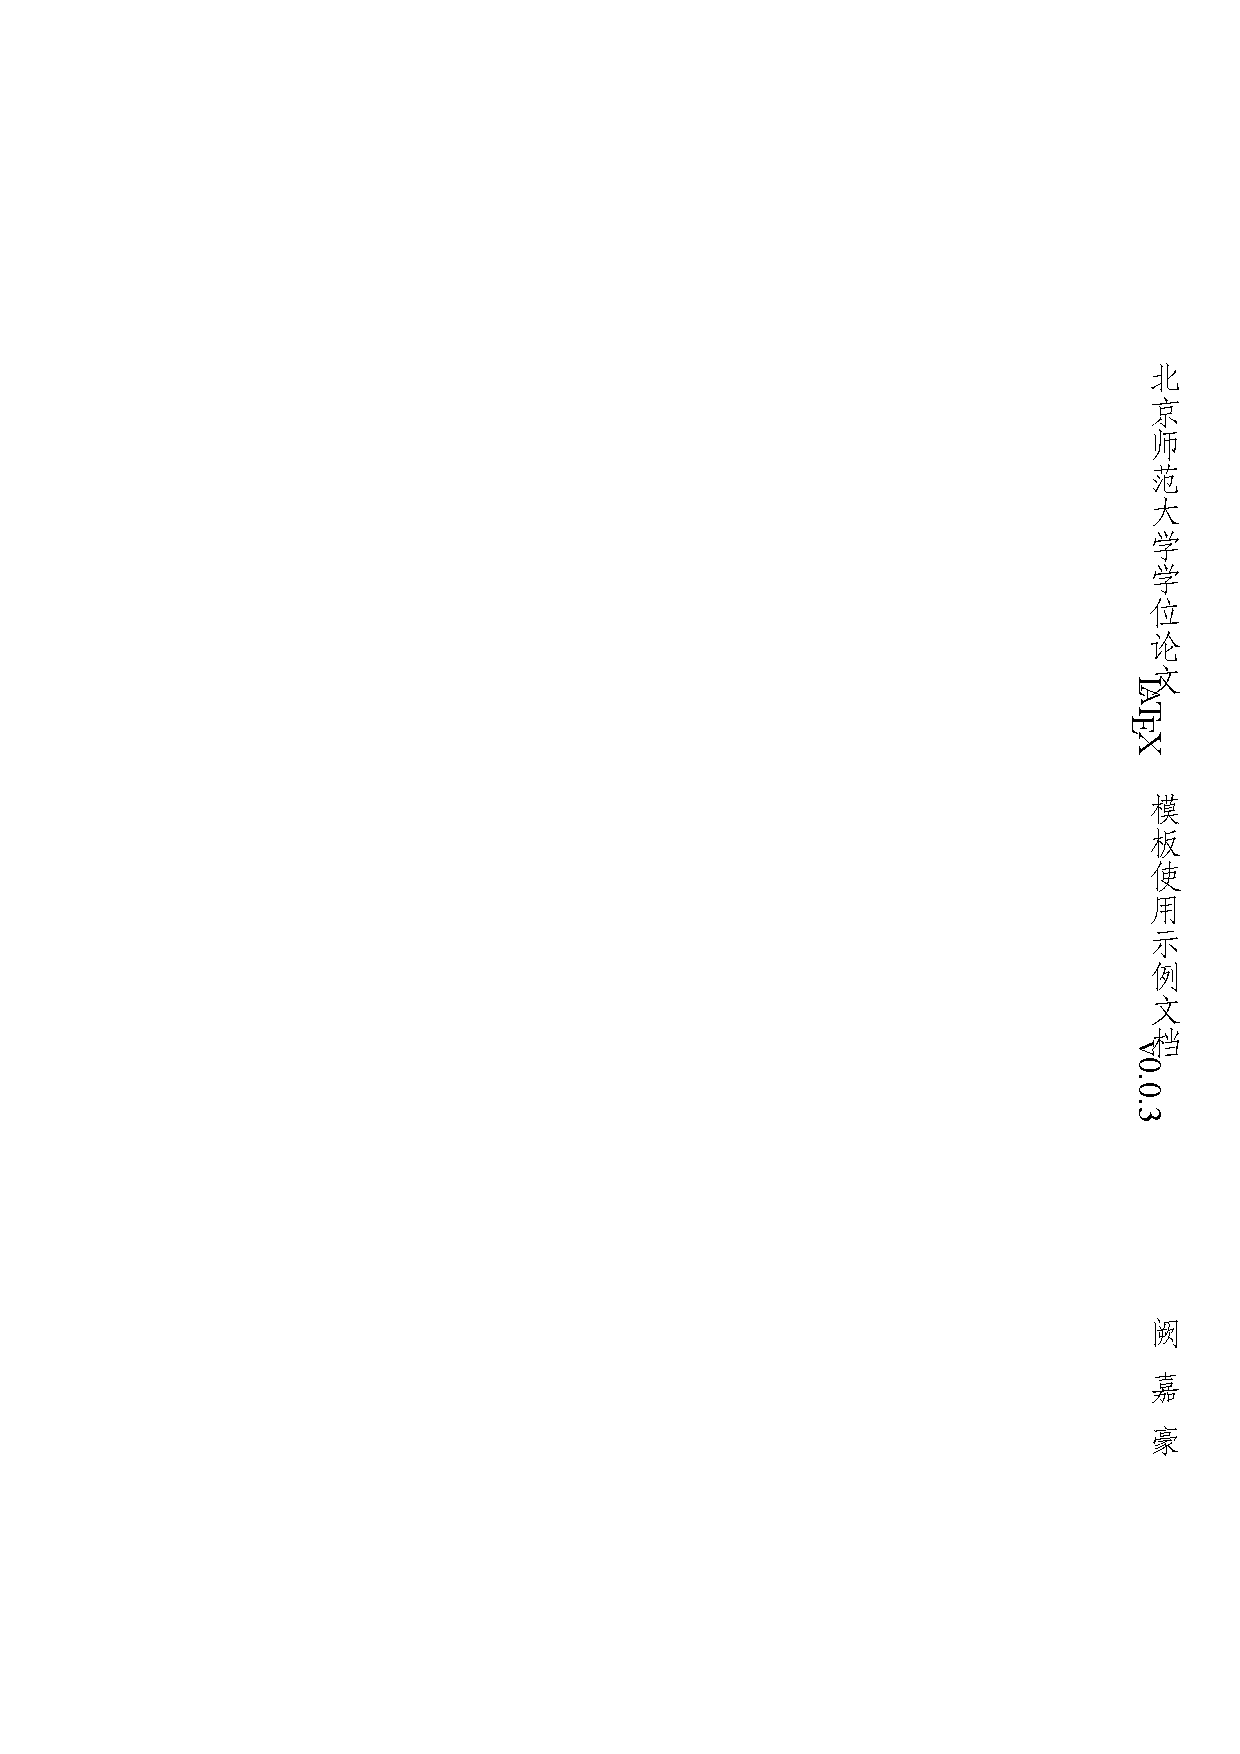
\includepdf[pages=1]{spine.pdf}%
}
\newcommand\bnu@spine{%
  \ifbnu@cjk@font@fandol
    \bnu@input@spine
  \else
    \ifbnu@cjk@font@noto
      \bnu@input@spine
    \else
      \spine
    \fi
  \fi
}
%    \end{macrocode}
% \end{macro}
%
%
% \subsection{其它}
% \label{sec:other}
%
% 借用 \cls{ltxdoc} 和 \cls{l3doc} 里面的几个命令方便写文档。
%    \begin{macrocode}
\DeclareRobustCommand\cs[1]{\texttt{\char`\\#1}}
\DeclareRobustCommand\file{\nolinkurl}
\DeclareRobustCommand\env{\textsf}
\DeclareRobustCommand\pkg{\textsf}
\DeclareRobustCommand\cls{\textsf}
%    \end{macrocode}
%
%    \begin{macrocode}
\sloppy
%</cls>
%    \end{macrocode}
%
%
% \iffalse
%    \begin{macrocode}
%<*dtx-style>
\ProvidesPackage{dtx-style}
\RequirePackage{hypdoc}
\RequirePackage{ifthen}
\RequirePackage{fontspec}[2017/01/20]
\RequirePackage{amsmath}
\RequirePackage{unicode-math}
\RequirePackage[UTF8,scheme=chinese]{ctex}
\RequirePackage[
  top=2.5cm, bottom=2.5cm,
  left=4cm, right=2cm,
  headsep=3mm]{geometry}
\RequirePackage{hologo}
\RequirePackage{array,longtable,booktabs}
\RequirePackage{listings}
\RequirePackage{fancyhdr}
\RequirePackage{xcolor}
\RequirePackage{enumitem}
\RequirePackage{etoolbox}
\RequirePackage{metalogo}
\RequirePackage[tightLists=false]{markdown}

\markdownSetup{
  renderers = {
    link = {\href{#2}{#1}},
  }
}

\hypersetup{
  pdflang     = zh-CN,
  pdftitle    = {BnuThesis:北京师范大学学位论文模板},
  pdfauthor   = {清华大学 TUNA 协会},
  pdfsubject  = {北京师范大学学位论文模板使用说明},
  pdfkeywords = {论文模板; 北京师范大学; 使用说明},
  pdfdisplaydoctitle = true
}%

\ifthenelse{\equal{\@nameuse{g__ctex_fontset_tl}}{mac}}{
  \setmainfont{Palatino}
  \setsansfont[Scale=MatchLowercase]{Helvetica}
  \setmonofont[Scale=MatchLowercase]{Menlo}
}{
  \setmainfont[
    Extension      = .otf,
    UprightFont    = *-regular,
    BoldFont       = *-bold,
    ItalicFont     = *-italic,
    BoldItalicFont = *-bolditalic,
  ]{texgyrepagella}
  \setsansfont[
    Extension      = .otf,
    UprightFont    = *-regular,
    BoldFont       = *-bold,
    ItalicFont     = *-italic,
    BoldItalicFont = *-bolditalic,
  ]{texgyreheros}
  \setmonofont[
    Extension      = .otf,
    UprightFont    = *-regular,
    BoldFont       = *-bold,
    ItalicFont     = *-italic,
    BoldItalicFont = *-bolditalic,
    Scale          = MatchLowercase,
    Ligatures      = CommonOff,
  ]{texgyrecursor}
}
\unimathsetup{
  math-style=ISO,
  bold-style=ISO,
}
\DeclareRobustCommand\mathellipsis{\mathinner{\unicodecdots}}
\IfFontExistsTF{XITSMath-Regular.otf}{
  \setmathfont[
    Extension    = .otf,
    BoldFont     = XITSMath-Bold,
    StylisticSet = 8,
  ]{XITSMath-Regular}
  \setmathfont[range={cal,bfcal},StylisticSet=1]{XITSMath-Regular.otf}
}{
  \setmathfont[
    Extension    = .otf,
    BoldFont     = *bold,
    StylisticSet = 8,
  ]{xits-math}
  \setmathfont[range={cal,bfcal},StylisticSet=1]{xits-math.otf}
}

\colorlet{bnu@macro}{blue!60!black}
\colorlet{bnu@env}{blue!70!black}
\colorlet{bnu@option}{purple}
\patchcmd{\PrintMacroName}{\MacroFont}{\MacroFont\bfseries\color{bnu@macro}}{}{}
\patchcmd{\PrintDescribeMacro}{\MacroFont}{\MacroFont\bfseries\color{bnu@macro}}{}{}
\patchcmd{\PrintDescribeEnv}{\MacroFont}{\MacroFont\bfseries\color{bnu@env}}{}{}
\patchcmd{\PrintEnvName}{\MacroFont}{\MacroFont\bfseries\color{bnu@env}}{}{}

\def\DescribeOption{%
  \leavevmode\@bsphack\begingroup\MakePrivateLetters%
  \Describe@Option}
\def\Describe@Option#1{\endgroup
  \marginpar{\raggedleft\PrintDescribeOption{#1}}%
  \bnu@special@index{option}{#1}\@esphack\ignorespaces}
\def\PrintDescribeOption#1{\strut \MacroFont\bfseries\sffamily\color{bnu@option} #1\ }
\def\bnu@special@index#1#2{\@bsphack
  \begingroup
    \HD@target
    \let\HDorg@encapchar\encapchar
    \edef\encapchar usage{%
      \HDorg@encapchar hdclindex{\the\c@HD@hypercount}{usage}%
    }%
    \index{#2\actualchar{\string\ttfamily\space#2}
           (#1)\encapchar usage}%
    \index{#1:\levelchar#2\actualchar
           {\string\ttfamily\space#2}\encapchar usage}%
  \endgroup
  \@esphack}

\lstdefinestyle{lstStyleBase}{%
   basicstyle=\small\ttfamily,
   aboveskip=\medskipamount,
   belowskip=\medskipamount,
   lineskip=0pt,
   boxpos=c,
   showlines=false,
   extendedchars=true,
   upquote=true,
   tabsize=2,
   showtabs=false,
   showspaces=false,
   showstringspaces=false,
   numbers=none,
   linewidth=\linewidth,
   xleftmargin=4pt,
   xrightmargin=0pt,
   resetmargins=false,
   breaklines=true,
   breakatwhitespace=false,
   breakindent=0pt,
   breakautoindent=true,
   columns=flexible,
   keepspaces=true,
   gobble=4,
   framesep=3pt,
   rulesep=1pt,
   framerule=1pt,
   backgroundcolor=\color{gray!5},
   stringstyle=\color{green!40!black!100},
   keywordstyle=\bfseries\color{blue!50!black},
   commentstyle=\slshape\color{black!60}}

\lstdefinestyle{lstStyleShell}{%
   style=lstStyleBase,
   frame=l,
   rulecolor=\color{purple},
   language=bash}

\lstdefinestyle{lstStyleLaTeX}{%
   style=lstStyleBase,
   frame=l,
   rulecolor=\color{violet},
   language=[LaTeX]TeX}

\lstnewenvironment{latex}{\lstset{style=lstStyleLaTeX}}{}
\lstnewenvironment{shell}{\lstset{style=lstStyleShell}}{}

\setlist{nosep}

\DeclareDocumentCommand{\option}{m}{\textsf{#1}}
\DeclareDocumentCommand{\env}{m}{\texttt{#1}}
\DeclareDocumentCommand{\pkg}{s m}{%
  \textsf{#2}\IfBooleanF#1{\bnu@special@index{package}{#2}}}
\DeclareDocumentCommand{\cls}{s m}{%
  \textsf{#2}\IfBooleanF#1{\bnu@special@index{package}{#2}}}
\DeclareDocumentCommand{\file}{s m}{%
  \nolinkurl{#2}\IfBooleanF#1{\bnu@special@index{file}{#2}}}
\newcommand{\myentry}[1]{%
  \marginpar{\raggedleft\color{purple}\bfseries\strut #1}}
\newcommand{\note}[2][Note]{{%
  \color{magenta}{\bfseries #1}\emph{#2}}}

\g@addto@macro\UrlBreaks{%
  \do0\do1\do2\do3\do4\do5\do6\do7\do8\do9%
  \do\A\do\B\do\C\do\D\do\E\do\F\do\G\do\H\do\I\do\J\do\K\do\L\do\M
  \do\N\do\O\do\P\do\Q\do\R\do\S\do\T\do\U\do\V\do\W\do\X\do\Y\do\Z
  \do\a\do\b\do\c\do\d\do\e\do\f\do\g\do\h\do\i\do\j\do\k\do\l\do\m
  \do\n\do\o\do\p\do\q\do\r\do\s\do\t\do\u\do\v\do\w\do\x\do\y\do\z
}
\Urlmuskip=0mu plus 0.1mu

\DeclareDocumentCommand{\githubuser}{m}{\href{https://github.com/#1}{@#1}}

\def\bnuthesis{\textsc{Bnu}\-\textsc{Thesis}}
%</dtx-style>
%    \end{macrocode}
% \fi
%
% \Finale
%
\endinput
% \iffalse
%  Local Variables:
%  mode: doctex
%  TeX-master: t
%  End:
% \fi
